\documentclass[11pt,oneside]{article}
\ifdefined\pdftrailerid\pdftrailerid{}\fi
\usepackage[T1]{fontenc}
\usepackage[utf8]{inputenc}
\usepackage{lmodern}
\pdfglyphtounicode{parenleftbig}{0028 FE01}
\pdfglyphtounicode{parenrightbig}{0029 FE01}
\pdfglyphtounicode{bracketleftbig}{005B FE01}
\pdfglyphtounicode{bracketrightbig}{005D FE01}
\pdfglyphtounicode{vextendsingle}{20D3}
\pdfglyphtounicode{parenleftbigg}{0028 FE03}
\pdfglyphtounicode{parenrightbigg}{0029 FE03}
\pdfglyphtounicode{bracketleftbigg}{005B FE03}
\pdfglyphtounicode{bracketrightbigg}{005D FE03}
\pdfglyphtounicode{parenleftBigg}{0028 FE04}
\pdfglyphtounicode{parenrightBigg}{0029 FE04}
\pdfglyphtounicode{bracketleftBigg}{005B FE04}
\pdfglyphtounicode{bracketrightBigg}{005D FE04}
\pdfglyphtounicode{braceleftBigg}{007B FE04}
\pdfglyphtounicode{bracerightBigg}{007D FE04}
\pdfglyphtounicode{parenlefttp}{239B}
\pdfglyphtounicode{parenrighttp}{239E}
\pdfglyphtounicode{bracketlefttp}{23A1}
\pdfglyphtounicode{bracketrighttp}{23A4}
\pdfglyphtounicode{bracketleftbt}{23A3}
\pdfglyphtounicode{bracketrightbt}{23A6}
\pdfglyphtounicode{bracelefttp}{23A7}
\pdfglyphtounicode{bracerighttp}{23AB}
\pdfglyphtounicode{braceleftbt}{23A9}
\pdfglyphtounicode{bracerightbt}{23AD}
\pdfglyphtounicode{braceleftmid}{23A8}
\pdfglyphtounicode{bracerightmid}{23AC}
\pdfglyphtounicode{parenleftbt}{239D}
\pdfglyphtounicode{parenrightbt}{23A0}
\pdfglyphtounicode{summationtext}{2211 FE01}
\pdfglyphtounicode{producttext}{220F FE01}
\pdfglyphtounicode{summationdisplay}{2211 FE02}
\pdfglyphtounicode{productdisplay}{220F FE02}
\pdfglyphtounicode{integraldisplay}{222B FE02}
\pdfglyphtounicode{bracketleftBig}{005B FE02}
\pdfglyphtounicode{bracketrightBig}{005D FE02}
\pdfglyphtounicode{floorleftBig}{230A FE02}
\pdfglyphtounicode{floorrightBig}{230B FE02}
\pdfglyphtounicode{radicalBig}{221A FE02}

\usepackage[margin=1in]{geometry}
\usepackage{amsmath,amssymb,amsthm,mathtools,mathrsfs}
\usepackage{booktabs,array,longtable}
\usepackage{microtype}
\usepackage{placeins}
\usepackage{needspace}
\usepackage{xcolor}
\usepackage{tikz}
\usetikzlibrary{arrows.meta,positioning,calc}
\usepackage{hyperref}
\hypersetup{hypertexnames=false,colorlinks=true,linkcolor=blue!45!black,citecolor=green!35!black,urlcolor=blue!55!black,pdftitle={Mass and covering exponents for fixed-length honeycomb walks},pdfauthor={OpenAI}}
\usepackage[capitalise,nameinlink,noabbrev]{cleveref}
\newtheorem{theorem}{Theorem}[section]
\newtheorem{lemma}[theorem]{Lemma}
\newtheorem{proposition}[theorem]{Proposition}
\newtheorem{corollary}[theorem]{Corollary}
\theoremstyle{definition}
\newtheorem{definition}[theorem]{Definition}
\theoremstyle{remark}
\newtheorem{remark}[theorem]{Remark}
\newcommand{\C}{\mathbb C}
\newcommand{\R}{\mathbb R}
\newcommand{\Z}{\mathbb Z}
\newcommand{\N}{\mathbb N}
\newcommand{\E}{\mathbb E}
\newcommand{\Prob}{\mathbb P}
\DeclareMathOperator{\diam}{diam}
\DeclareMathOperator{\tr}{tr}
\DeclareMathOperator{\supp}{supp}
\DeclareMathOperator{\dist}{dist}
\DeclareMathOperator{\Var}{Var}
\allowdisplaybreaks[2]
\setlength{\emergencystretch}{2em}
\title{Mass and covering exponents for fixed-length honeycomb walks}
\author{OpenAI}
\date{September 26, 2026}
\begin{document}
\maketitle
\begin{abstract}
For uniform self-avoiding walks of every sufficiently large integer length on the honeycomb lattice, we prove diameter exponent $3/4$ and simultaneous local-mass and covering exponent $4/3$, with arbitrary positive exponent slack and arbitrary polynomial failure probability.
\end{abstract}
\section{Introduction}\label{sec:introduction}
A self-avoiding walk is a nearest-neighbor lattice path that visits no vertex twice. Its length is fixed combinatorially, but its spatial extent is random. The exponent $3/4$ expresses a predicted relation between those two quantities in two dimensions; its reciprocal $4/3$ expresses the corresponding mass dimension. A precise statement requires both a probability law and a choice of spatial statistic. This paper concerns the regular honeycomb lattice and gives such a statement for diameter, local mass, and covering numbers.

\subsection{The model and the meaning of the exponents}
Let $\mathbb H$ be the planar dual of the equilateral triangular tiling with triangle side length one. Fix a vertex $o$. Let $\mathcal W_n$ be the set of paths
\[
\gamma=(\gamma_0,\ldots,\gamma_n),\qquad \gamma_0=o,
\]
whose consecutive vertices are adjacent in $\mathbb H$ and whose vertices are all distinct. Write $c_n=|\mathcal W_n|$, and let $\Prob_n$ be the uniform law on $\mathcal W_n$. The endpoint $\gamma_n$ is free. We use the Euclidean embedding and set
\[
V(\gamma)=\{\gamma_0,\ldots,\gamma_n\},\quad
D(\gamma)=\diam V(\gamma),\quad
M_\gamma(z,s)=|V(\gamma)\cap\overline B(z,s)|.
\]
Let $\mathcal N_\gamma(s)$ be the least number of closed Euclidean balls of radius $s$ that cover $V(\gamma)$; their centers may lie anywhere in the plane.

\begin{theorem}[Fixed-length mass and covering exponents]\label{thm:main}\label{09_fast_paths:fixed-length}
For every $\delta>0$ and $k>0$, there are constants $C_{\delta,k}<\infty$ and $n_0(\delta,k)$ such that, for every integer $n\ge n_0(\delta,k)$, an event of $\Prob_n$-probability at least $1-C_{\delta,k}n^{-k}$ has all the following properties:
\begin{align}
 n^{3/4-\delta}&\le D(\gamma)\le n^{3/4+\delta},\label{eq:main-diameter}\\
 n^{-\delta}\min\{n,s^{4/3}\}
 &\le M_\gamma(z,s)\le n^{\delta}\min\{n,s^{4/3}\},\label{eq:main-mass}\\
 n^{-\delta}(1+ns^{-4/3})
 &\le \mathcal N_\gamma(s)\le n^{\delta}(1+ns^{-4/3}).\label{eq:main-cover}
\end{align}
The last two bounds hold simultaneously for every $z\in V(\gamma)$ and every real $s\in[1,n]$ (with $z$ relevant only to \eqref{eq:main-mass}).
\end{theorem}
The power slack absorbs constants and the difference between $n$ edges and $n+1$ vertices. In particular, the notation $n^{a+o(1)}$ below always has an explicitly stated probability interpretation; it does not assert a limiting multiplicative constant.

\begin{corollary}[Span in every lattice normal]\label{cor:directional-span}
For every \(\delta,k>0\), outside an event of \(\Prob_n\)-probability
\(O_{\delta,k}(n^{-k})\), the projection of \(V(\gamma)\) onto each
unit normal to a direction of triangular-lattice edges has span at least
\(n^{3/4-\delta}\). This holds for every sufficiently large integer \(n\).
\end{corollary}
This lower bound in each of the three normal directions gives more
information than a lower bound on the largest spatial extent.

\begin{corollary}[Covering dimension at polynomially separated scales]\label{cor:dimension}
For each fixed $\epsilon\in(0,3/4)$,
\[
\sup_{1\le s\le n^{3/4-\epsilon}}
\left|\frac{\log\mathcal N_\gamma(s)}{\log(D(\gamma)/s)}-\frac43\right|
\longrightarrow0
\quad\hbox{in }\Prob_n\hbox{-probability}.
\]
The statistic can be defined arbitrarily when $D(\gamma)\le n^{3/4-\epsilon}$.
\end{corollary}

\begin{corollary}[Radius of gyration and moments]\label{cor:gyration}
Let
\[
\bar\gamma=\frac1{n+1}\sum_{j=0}^n\gamma_j,
\qquad R_g(\gamma)^2=\frac1{n+1}\sum_{j=0}^n|\gamma_j-\bar\gamma|^2.
\]
Then $R_g=n^{3/4+o(1)}$ with the same arbitrary polynomial probability convention as in Theorem~\ref{thm:main}. For every fixed $p>0$,
\[
\E_n[D^p]=n^{3p/4+o(1)},\qquad
\E_n[R_g^p]=n^{3p/4+o(1)}.
\]
\end{corollary}
We prove the deductions from the geometric estimates, including the Corollaries, in Section~\ref{sec:fixed-length}. These statements concern the mass and covering behavior of the lattice trace as its length grows. The assertions do not include convergence to a continuum curve, a continuum Hausdorff dimension, a universality theorem on changing lattice, or a fixed-length lower bound on $|\gamma_n-o|$. A lower bound for the diameter does not imply that the two endpoints are far apart.


\subsection{Critical weights and the geometric argument}
The proof first works with the critical activity
\(\rho=(2+\sqrt2)^{-1/2}\). A path then carries weight \(\rho^\ell\),
where \(\ell\) counts edges for a vertex-rooted walk and visited vertices
for a path whose endpoints are ports, the midpoints of honeycomb edges. A \emph{mass} is a sum of
these weights before normalization. The distinction lets pieces in
adjacent open strips concatenate with exactly the product weight.
A bridge crosses a strip without visiting either boundary elsewhere.
It is irreducible if no intermediate lattice line parallel to the strip
boundaries is crossed exactly once; such a line would split it into two
bridges.

Exact lattice observables provide the mass crossing a strip, nesting
around a face, the length-square mass of polygons, and a uniform bound
for arcs joining two marked ports on a cylinder. We state their precise
positive outputs in Section~\ref{sec:inputs}. The analytic proofs belong
to the complete companion articles identified there. Here we prove the
geometric passage from those inputs to an unrestricted fixed-length trace.

There are three obstacles. A bridge used to modify a path must fit in a
corridor that avoids the remaining pieces; a strip mass or mean length
alone gives no such guarantee. We sew smaller bridges and recover the
sewing lines from the resulting path, controlling the multiplicity of
that operation. This produces localized first and second moments and,
by Cauchy--Schwarz, a subpower chance of seeing a long bridge. Independent
renewal trials amplify that chance. An exact conditioning identity then
transfers the estimate to a bridge of a specified height.

Next, one bridge estimate must control all subpaths of an arbitrary
walk. Ordered tests of adjacent renewal paths suppress both unusually
fast travel and excessive length in a narrow region. When the two tests
meet the same irreducible piece, its entire weight enters once. This
joint estimate is essential when the number of turns grows with the
scale. Finally, a separate estimate for many disjoint crossings controls
repeated visits to one ball. A subpath bound on its own would leave these
separate visits uncontrolled.

The estimates are proved for rooted walks of any length confined to
diameter at most a fixed multiple of \(H\). For every \(\tau>0\),
they simultaneously bound the length of every subwalk \(\sigma\) by
\(H^\tau(1+\operatorname{diam}\sigma)^{4/3}\), its diameter by
\(H^\tau(1+|\sigma|)^{3/4}\), and the number of visited vertices
in a ball of radius \(s\) about a visited vertex by \(H^\tau s^{4/3}\)
for \(1\le s\le H\). Here \(|\sigma|\) counts edges. For every
\(A>0\), the total critical mass of walks violating any of these
bounds is at most \(C_{\tau,A}H^{-A}\). This absolute estimate is
strong enough to survive summation over all the possible subpaths.

To pass to every integer length, submultiplicativity and the polynomial
strip lower bound give \(c_n\rho^n\ge1\). Taking \(H\) proportional
to \(n\) and dividing an exceptional mass by this fixed-length
partition function preserves arbitrary polynomial decay. The diameter,
local mass and covering conclusions then follow on one simultaneous event.
The elementary renewal process needed here is developed locally; no
change-of-ensemble theorem is assumed.

The proof follows these steps in order. Section~\ref{sec:full-box}
first bounds the mass of the outside pieces that a cut leaves behind.
Section~\ref{sec:08-sewing-renewal} proves the confined bridge length
moments and then constructs turning corridors for the later probes.
Section~\ref{sec:renewal} amplifies the moment bound at a specified
height. Section~\ref{sec:10-thermal-probes} then controls
ordered adjacent paths, including a shared long irreducible.
Sections~\ref{sec:fast} and~\ref{sec:11-slow-covering} use those estimates
to bound fast travel, excessive local length, and repeated visits.
Section~\ref{sec:fixed-length} performs the exact-length transfer and
proves the stated geometric consequences. The independent asynchronous
avoidance argument is retained in Appendix~\ref{sec:asynchronous}.


\subsection{Historical context}
The predicted exponent $3/4$ belongs to the two-dimensional polymer
theory developed through the dilute $O(n)$ model. Nienhuis's
solid-on-solid and Coulomb-gas analysis gives this exponent at $n=0$
\cite{Nienhuis1982}. These predictions concern more than the exponential
growth rate of the number of walks. Duminil-Copin and Smirnov proved the
exact honeycomb connective constant by introducing a parafermionic
observable and summing its local cancellation over a strip
\cite{DCS2012}. Their argument gives $c/T\le B_T\le1$ for the critical
strip-crossing mass; the sharper exponent $-1/4$ is recorded there as a
prediction.

Subsequent work sharpened the information about this mass.
Beaton, Bousquet-M\'elou, de Gier, Duminil-Copin and Guttmann proved
$B_T\to0$ in their study of surface adsorption \cite{BeatonEtAl2014}.
Glazman and Manolescu gave a shorter proof and a logarithmic subsequence
bound, and established invariance of the boundary two-point function
for a specified class of columnwise rhombic half-plane tilings
with integrable weights \cite{GlazmanManolescu2020}. More recently,
Krachun and Panagiotis proved
a polynomial upper bound on $B_T$ and a quantitative sub-ballistic
estimate: a uniform $n$-step honeycomb walk stays within distance
$C n/\log(n+1)$ of its origin except on an event of probability at most
$\exp(-c n^{2/3})$ \cite{KrachunPanagiotis2026}.

The analytic companions used here provide the further quantitative strip
and marked-polygon estimates needed for the geometric argument.

The bridge factorization follows Kesten's renewal method
\cite{Kesten1963}; see also Madras and Slade~\cite{MadrasSlade1993}
and the appendix of Lawler, Schramm and Werner~\cite{LSW2004}.
Dyhr, Gilbert, Kennedy, Lawler and
Passon~\cite[Proposition 2.10]{DyhrEtAl2011} identify the critical
free-endpoint strip law on the square lattice by conditioning the
infinite half-plane walk to have a cut at a prescribed height and
taking its prefix through the upper strip boundary.
We derive the renewal normalization and this finite-height identity
in the present port convention. For the final full-plane law at each
integer length, we use absolute exceptional masses and the
partition-function bound \(c_n\rho^n\ge1\).

Lawler, Schramm and Werner also proposed a continuum description through
\(\mathrm{SLE}_{8/3}\), whose Hausdorff dimension they identified as
\(4/3\) \cite[Proposition 2(ii)]{LSW2004}. Beffara subsequently proved
the general formula \(\min\{2,1+\kappa/8\}\) for the dimension of
\(\mathrm{SLE}_{\kappa}\) \cite{Beffara2008}.
These continuum results explain the predicted mass dimension;
a lattice scaling limit is neither an input nor an output of the
present proof.

\section{Critical masses and the analytic inputs}\label{sec:inputs}
Our geometric arguments use positive sums of walk and polygon weights.
This section fixes their endpoint conventions and states the precise
analytic estimates proved in the companion papers. A free endpoint always
means a sum over the actual possible endpoint ports from one fixed source;
it never introduces a second translation sum.

\subsection{Ports, strips and local endpoint changes}
A port is the midpoint of an edge of the triangular tiling. A port path
follows honeycomb edges, with an initial and a final half-edge, and visits
each dual vertex at most once. A nonempty port path has distinct endpoint
ports; the empty height-zero bridge below is the sole exception. Its
length counts visited vertices and its
weight is \(w(\gamma)=\rho^{|\gamma|}\), with
\(\rho=(2+\sqrt2)^{-1/2}\). The trace of a port path includes its two
ports. Removing these ports changes its diameter by a bounded constant.
Unrestricted vertex paths keep the edge-count convention of the introduction.

A horizontal band is the region between two successive horizontal lines
of tiling edges. Its Euclidean height is \(d_0=\sqrt3/2\).
A strict bridge of height \(h\) goes from a bottom port to a top port of
the open \(h\)-band strip and has no other visit to the boundary.
An arch has two distinct ports on the same boundary. Because ports carry
no weight and adjacent open strips have disjoint vertices, concatenating
strict bridges multiplies their weights exactly. Every horizontal seam
port is a translate of the initial port by a symmetry of the triangular
tiling, with its inward half-edge pointing into the next band. Thus each
translated continuation has exactly the same admissible shapes and weights;
there is no residual port type or parity state in this concatenation. Tangential displacements
of height-\(h\) bridges lie in \(h/2+\Z\). Write
\[
 b_h(x)=\sum_{\gamma:0\to(x,h)}w(\gamma),\qquad
 B_h=\sum_xb_h(x),\qquad B_0=1.
\]
We write \(\Prob_h^{\rm br}\) for the probability measure obtained by
dividing these bridge weights by \(B_h\). Let \(K_h(j)\) be the
arch mass between bottom ports separated by the nonzero integer \(j\),
and put \(A_h=\sum_{j\ne0}K_h(j)\) and
\(m_h=\sum_{j>0}jK_h(j)\).

A weak bridge is a vertex path whose endpoints attain its minimum and
maximum heights; intermediate visits to these levels are permitted.
The following bounded modification will be used whenever a geometric
cut produces a vertex endpoint.
\begin{lemma}[Endpoint extension]\label{lem:port-extension}
A weak bridge in any lattice normal direction can be extended to a strict
port bridge between the first lattice boundary lines outside its height
range. The height and length change by \(O(1)\), the weight ratio is
bounded above and below by positive constants, and the inverse operation
has bounded multiplicity after recording its endpoint types.
\end{lemma}
\begin{proof}
At a lower endpoint whose triangle center is nearest its lower side,
append the vertical half-edge to that side's port. At the other triangle
type, first append its fixed downward edge and then the vertical half-edge.
The reflected operation applies at the upper endpoint. Every newly added
vertex lies strictly outside the old height range, so it was unvisited.
The two additions are disjoint for positive macroscopic span. Bounded
spans have only finitely many endpoint types and use the same construction;
a zero-span piece is trivial. At most three extra vertex factors occur
relative to the original edge count. Removing the recorded one- or
two-edge endpoint patterns recovers the original path, proving all bounds.
Rotations and reflections give the other lattice normal directions.
\end{proof}

Throughout, a bound \(F(h)\le h^{a+o(1)}\) means that for each
\(\epsilon>0\), \(F(h)\le C_\epsilon h^{a+\epsilon}\) for all
sufficiently large \(h\). The corresponding lower bound has the analogous
meaning. Constants may depend on declared fixed geometry and on exponent
slack. Uniform statements retain one choice of constant over their full
stated parameter range.

\subsection{Strip flux and nesting}
Set \(c=\cos(3\pi/8)\). The first input is the positive boundary
consequence of the parafermionic observable, together with its quantitative
strip refinement. We use the complete statements of
\cite[Theorem 1.1 and Lemma 2.1]{StripCompanion}.
\begin{theorem}[Boundary flux and strip mass]\label{thm:01-strip}\label{lem:01-boundary}
For every finite simply connected union \(D\) of triangular tiles with
simple polygonal boundary and each boundary source port \(a\),
\[
 \sum_{b\in\partial D}\sum_{\gamma:a\to b}
       \rho^{|\gamma|}e^{3iW(\gamma)/8}=1,
\]
where \(W\) is total signed turning from the initial inward direction to
the final outward direction. If \(D\) is convex, its unsigned exit mass
is at most \(1/c\). For each \(h\ge1\), all strip sums defined above
are finite and
\[
 cA_h+B_h=1,\qquad B_{h+1}\le B_h,\qquad
 B_h\asymp(1+h)^{-1/4},\qquad
 m_h\asymp h^{3/4},\qquad m_{h+1}-m_h\asymp B_h.
\]
The constants are independent of \(h\), and \(b_h(x)=b_h(-x)\).
\end{theorem}
The exact identity and monotonicity, rather than the bridge power alone,
will control convex cuts and variation of the endpoint kernel.

For an internal honeycomb mid-edge \(p\) in a convex domain \(D\),
let \(L_p(D)\) be the sum over ordered boundary chords through \(p\),
weighted by \(\rho^{|\gamma|}\cos(3W(\gamma)/8)\). A polygon nest
around a face center \(f\) is a finite set of pairwise vertex-disjoint
simple polygons, each strictly enclosing \(f\). Its weight is the
product of \(2\rho^{|\ell|}\) over its polygons, and the empty nest
has weight one. Write \(Z_f(D)\) for the nesting mass in \(D\).
Let \(P_2(r)\) denote the whole-plane nesting mass with every polygon's
diameter at most \(r\), and let \(S_k\) denote the middle-face nesting
mass in a strip of \(2k\) bands.
\begin{theorem}[Length and nesting]\label{lem:02-length-nests}\label{thm:05-nest-normalization}
For the two face centers \(f_1,f_2\) adjacent to \(p\),
\[
 \frac1{\sqrt2}\bigl(Z_{f_1}(D)+Z_{f_2}(D)\bigr)
 \le L_p(D)\le Z_{f_1}(D)+Z_{f_2}(D).
\]
The same comparison holds with finite quantities in every infinite strip
of fixed positive height. Moreover,
\(P_2(r)=r^{1/12+o(1)}\) and \(S_k=k^{1/12+o(1)}\).
\end{theorem}
These are the length--nest and planar-normalization theorems of
\cite[Lemma 11.4, Theorem 11.2 and Corollary 11.3]{CylinderCompanion}. We will place diameter-truncated nests in the
interior of a finite triangle; an untruncated planar partition function
would not give that inclusion.
\begin{theorem}[Raw strip first-length mass]\label{prop:02-length-reduction}
From one fixed bottom port of the \(h\)-band strip,
\[
 \sum_{\gamma\text{ arch or bridge}}\rho^{|\gamma|}|\gamma|
       \le h^{13/12+o(1)}.
\]
\end{theorem}
The sum is unnormalized and includes paths ending on either boundary.
It is Proposition 11.5 of \cite{CylinderCompanion}; it is
stronger information for our purpose than a mean conditional on reaching
a deep line. The main geometric proof will supply a matching lower
first moment on bridges confined to diameter at most a fixed multiple
of their height.

\subsection{Marked polygons and arcs}
The marked-polygon theorem of \cite[Theorem 1.1]{MarkedCompanion} gives
\begin{theorem}[Polygon length-square mass]\label{thm:07_magnetic_analysis-moment}
For unrooted, unoriented simple honeycomb polygons modulo triangular-lattice
translations,
\[
 \sum_{[\ell]:\,\operatorname{diam}\ell\le H}
             \rho^{|\ell|}|\ell|^2\le H^{2/3+o(1)}.
\]
\end{theorem}
Here \(|\ell|\) is its vertex count. The translation-class convention
is needed when an exterior closure is translated back to a rooted path.

We also use the cylinder arc estimate of \cite[Theorem 8.3]{MarkedCompanion}.
Its cylinder is
formed by a row cut in cyclic order \([p,X,p',Y]\), where \(p,p'\)
are two marked ports and \(X,Y\) are sets of ordinary sites. Put
\(s=|X|\), \(b=|Y|\), and require \(s+b+2\) even. The physical row
uses rhombus parameters \(\lambda=\pi/8\) or \(2\lambda\): these
two parameter values label the two lattice side directions forming the
positive cone. After a
common shift the logarithmic parameters \(a_i\) have imaginary heights
\(0\) or \(\beta=\pi/4\) in \(X\) and at the marks, and height
zero in \(Y\). At these physical parameters all real parts of the
shifted \(a_i\) are zero. An upper site is one of height \(\beta\). Let
\(A(p,p')\) be the unnormalized critical mass of self-avoiding cylinder
arcs departing west from \(p\) and arriving east at \(p'\), making no
other visit to either mark and leaving their unused half-edges vacant.
\begin{theorem}[Uniform one-arc bound]\label{09_fast_paths:one-arc-bound}
There are constants \(\delta_1>0\), \(L_*>0\), and \(C<\infty\)
such that \(A(p,p')\le b^C\) whenever
\[
 L_Y\ge L_X\ge L_*,\qquad s\le b,\qquad
 L_X=\tfrac34\log s,\quad L_Y=\tfrac34\log b,
\]
and at least fraction \(1/2-\delta_1\) of the ordinary \(X\)-sites
are upper. There is no positive lower bound on \(L_X/L_Y\).
\end{theorem}
The exponent \(C\) is fixed throughout this domain. In the next section
we construct such a row cut from an arbitrary walk in a box. There
\(s\) may stay bounded while \(b\) grows with the box, which explains
why a comparable-wall estimate would not suffice.

\subsection{A tail for every polygon count}
The final input is different from the length-square bound. On the
balanced physical two-marker cylinder with even \(N=2m\), use the
parameter \(2\lambda\) on its first \(m\) bands and \(\lambda\)
on the remaining \(m\) bands. Let \(w_N(a)\) be the critical mass of
families of exactly \(a\) disjoint separating polygons, namely
\[
 w_N(a)=\sum_{\substack{\mathcal F\text{ disjoint, separating}\\
                         \#\mathcal F=a}}
               \prod_{P\in\mathcal F}\rho^{|P|}.
\]
There is no factor two per polygon in this definition. The all-count
tail bound of \cite[Corollary 8.2]{CylinderCompanion} states that, uniformly for
every integer \(a\ge0\),
\begin{equation}\label{eq:input-cylinder-tail}
 w_N(a)\le \exp\left(C\log N-\frac{ca^2}{\log N}\right)
\end{equation}
for sufficiently large even \(N\). Its proof uses the all-real-fugacity estimate of
\cite[Theorem 8.1]{CylinderCompanion}, namely the bound
\(Z_N(2\cosh v)\le\exp(C\log N(1+v^2))\) for every real \(v\ge0\).
An asymptotic for bounded fugacity would not justify arbitrarily large
\(a\). We use \eqref{eq:input-cylinder-tail} only after an explicit
reflection and concatenation has turned prescribed slab crossings into
such polygon families.

\section{The critical mass of paths in a box}\label{sec:full-box}
The later proofs extract a special subpath and sum freely over the two
outside pieces. We therefore need a bound that sums \emph{all} lengths
and endpoints in the containing box, with one fixed polynomial exponent.
The one-arc estimate in Theorem~\ref{09_fast_paths:one-arc-bound} supplies
that bound after a geometric reduction. Its uniformity when one group of
bands stays fixed while the other grows is used in the last step.

\begin{proposition}[Full-box susceptibility]\label{09_fast_paths:full-box}
Let \(S(H)\) be the maximum, over starting vertices in a box of side
\(H\), of the critical mass of walks confined to that box, with
arbitrary endpoint and length. There are constants \(C_0,C_1\) such
that \(S(H)\le C_0(1+H)^{C_1}\).
\end{proposition}
\begin{proof}
\emph{The suffix test.}
We first choose a small constant \(a>0\), and later choose a sufficiently
large \(W\), once and independently of \(H\). Put
\(m=\lfloor aW\rfloor\). Walks shorter than \(m\) cost
\(\exp(O(W))\). Consider the finitely many triangular bases, including
reflections, whose upward side directions span a \(60^\circ\) cone.
In each basis require a westward step among the last \(m\) steps.
If this fails in one basis, there is at most one eastward and one
bisector-parallel choice at each vertex. Two consecutive parallel choices
would immediately backtrack. Thus the number of length-\(l\)
continuations avoiding west is at most \(C\varphi^l\), where
\(\varphi=(1+\sqrt5)/2\). Since \(\rho\varphi<1\), the total mass
failing at least one of these suffix tests is at most
\begin{equation}\label{eq:fullbox-suffix}
 \epsilon_W S(H),\qquad
 \epsilon_W=C(\rho\varphi)^m.
\end{equation}
The prefix ending where the suffix starts is included in \(S(H)\);
ignoring its avoidance constraints only enlarges this bound.

\smallskip\noindent\emph{Finding a cylinder arc.}
We seek a middle arc from a suitable earlier step to a westward step in
the suffix. The criterion below makes this arc eligible for the one-arc
theorem. Choosing the first such step leaves a prefix with no earlier
qualifying step; after treating the arc, we will bound the mass of these
prefixes by a constant depending only on \(W\).
Fix the endpoint \(z\), costing \(O((1+H)^2)\) choices, and scan the
step midpoints before this suffix. Let \(\ell_1,\ell_2,\ell_3\) be the
three lattice-side lines through \(z\), and put
\(d(p)=\min_i\operatorname{dist}(p,\ell_i)\). If \(d(p)>W\), the
vector \(q=z-p\) lies in one open positive cone. Write
\[
 q=u_1e_1+u_2e_2,
 \qquad u_1,u_2\ge 2W/\sqrt3,
 \qquad t=\frac{u_1}{u_1+u_2},
\]
where \(e_1,e_2\) are its adjacent unit triangular side vectors. The
coefficient bounds follow by taking distances to the two cone-side lines.
Assignment \(A\) makes \(e_1\) the upper-angle direction and is eligible
when \(t\ge r\), where \(r=1/2-\delta_1/2\). The reflected assignment
\(B\) makes \(e_2\) upper and is eligible when \(t\le1-r\). Reflection
fixes the cone bisector and reverses the transverse coordinate. In
particular, a step with negative transverse increment is westward in
\(A\), a step with positive increment is westward in \(B\), and a
bisector-parallel step is westward in neither. Call a step successful
if it is westward in some eligible assignment.

Suppose there is a success, and use the first one, with midpoint \(p\).
Choose a westward suffix step in its eligible basis, with midpoint \(p'\).
The intervening arc departs west from \(p\) and arrives east at \(p'\).
Moreover \(p'-p=q+O(m)\). The two marked triangular sides have types
\(\tau,\tau'\in\{1,2\}\); write
\(p=v+e_\tau/2\) and \(p'=v'+e_{\tau'}/2\), where \(v,v'\) are
triangular lattice vertices. The displacement between the two marked
half-sides is
\begin{equation}\label{eq:fullbox-integer-row}
 n_1e_1+n_2e_2
   =(p'-p)-\frac{e_\tau+e_{\tau'}}2
   =v'-v-e_\tau.
\end{equation}
Thus \(n_1,n_2\) are integers, since adjacent side vectors form an
integer lattice basis. They satisfy
\(n_i\ge cW-Cm-1\), and \(s=n_1+n_2\le C(H+1)\).
The change in the upper coefficient fraction is at most
\(C(m+1)/W\). Choose \(a\) small relative to \(\delta_1\), and then
\(W\) large. Both coefficients are positive, \(s\ge cW\), and the
ordinary upper fraction is at least \(1/2-\delta_1\).

Figure~\ref{fig:fullbox-cone-row} shows the cone and the marked
half-sides in this displacement calculation.
\begin{figure}[htbp]
\centering
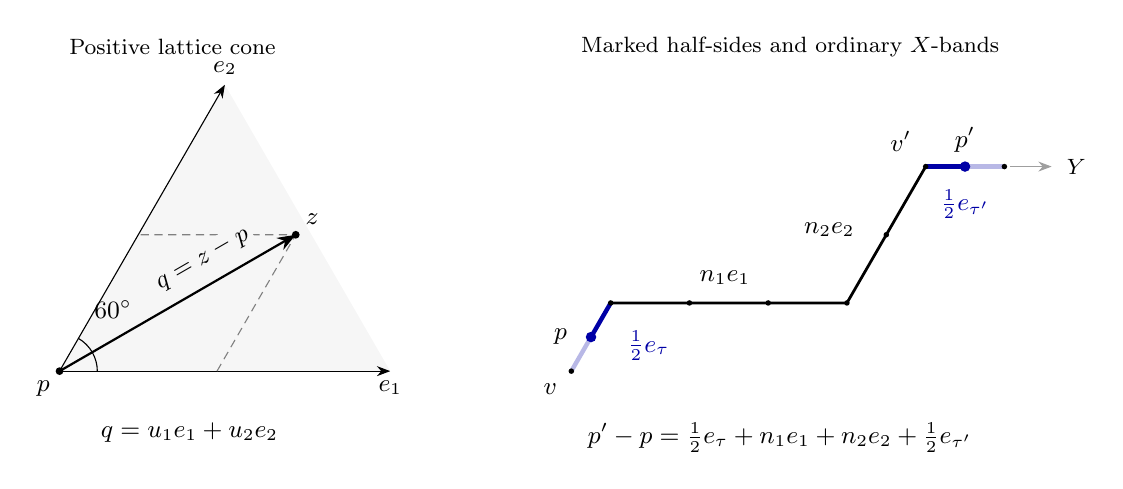
\begin{tikzpicture}[x=1cm,y=1cm,font=\small,>=Stealth,
  row/.style={line width=1pt,line join=round},
  marker/.style={line width=1.6pt,blue!65!black}]
 \begin{scope}
  \coordinate (p) at (0,0);
  \coordinate (q) at (3,1.732);
  \fill[gray!7] (p)--(4.20,0)--(2.10,3.637)--cycle;
  \draw[->] (p)--(4.20,0) node[below] {$e_1$};
  \draw[->] (p)--(2.10,3.637) node[above] {$e_2$};
  \draw[densely dashed,gray] (2,0)--(q)--(1,1.732);
  \draw[->,line width=.8pt] (p)--(q);
  \fill (p) circle (1.4pt) node[below left] {$p$};
  \fill (q) circle (1.4pt) node[above right] {$z$};
  \draw (.48,0) arc (0:60:.48);
  \node at (.68,.78) {$60^\circ$};
  \node[rotate=30,fill=gray!7,inner sep=1.5pt] at (1.82,1.42) {$q=z-p$};
  \node[anchor=west,font=\footnotesize] at (0,4.12) {Positive lattice cone};
  \node[anchor=north] at (1.65,-.53) {$q=u_1e_1+u_2e_2$};
 \end{scope}
 \begin{scope}[xshift=6.5cm]
  \coordinate (v) at (0,0);
  \coordinate (p) at (.25,.433);
  \coordinate (w) at (.5,.866);
  \coordinate (vp) at (4.5,2.598);
  \coordinate (pp) at (5,2.598);
  \coordinate (end) at (5.5,2.598);
  \draw[marker,opacity=.28] (v)--(p);
  \draw[marker] (p)--(w);
  \draw[row] (w)--(3.5,.866)--(vp);
  \draw[marker] (vp)--(pp);
  \draw[marker,opacity=.28] (pp)--(end);
  \foreach \x/\y in {0/0,.5/.866,1.5/.866,2.5/.866,3.5/.866,4/1.732,4.5/2.598,5.5/2.598}
    \fill (\x,\y) circle (1pt);
  \fill[blue!65!black] (p) circle (1.9pt);
  \fill[blue!65!black] (pp) circle (1.9pt);
  \node[anchor=east] at (.07,.44) {$p$};
  \node[anchor=south] at (5,2.66) {$p'$};
  \node[anchor=north east] at (-.06,-.04) {$v$};
  \node[anchor=south east] at (4.44,2.67) {$v'$};
  \node[anchor=south] at (1.95,.98) {$n_1e_1$};
  \node[anchor=east] at (3.72,1.80) {$n_2e_2$};
  \node[anchor=west,text=blue!65!black] at (.59,.32) {$\tfrac12e_\tau$};
  \node[text=blue!65!black] at (5.0,2.12) {$\tfrac12e_{\tau'}$};
  \draw[->,gray!75] (5.57,2.598)--(6.10,2.598);
  \node[anchor=west,font=\footnotesize] at (6.17,2.598) {$Y$};
  \node[anchor=west,font=\footnotesize] at (0,4.12) {Marked half-sides and ordinary $X$-bands};
  \node[anchor=north,align=center] at (2.65,-.53)
    {$p'-p=\tfrac12e_\tau+n_1e_1+n_2e_2+\tfrac12e_{\tau'}$};
 \end{scope}
\end{tikzpicture}
\caption{The row construction in a positive $60^\circ$ lattice cone.
On the right, an example canonical order uses $n_1=3$ ordinary sides in
direction $e_1$, followed by $n_2=2$ in direction $e_2$; the marked
sides have types $\tau=2$ and $\tau'=1$. The segment from $p$ to
$p'$ contains one half of each marked side, so subtracting these
halves leaves the integer displacement $n_1e_1+n_2e_2$.
The faint halves complete the marked sides but do not belong to this
segment. This is a row cut, not the extracted honeycomb arc; the arc
may cross ordinary parts of the row. The angles drawn are Euclidean
lattice angles, not the spectral parameters.}
\label{fig:fullbox-cone-row}
\end{figure}


Use these integers as the ordinary \(X\)-band counts in the row
\([p,X,p',Y]\), in a fixed canonical order. We do not sum over band
orders. Choose all \(b\) ordinary \(Y\)-bands lower, with
\(b\ge K(H+s+1)\), adjusting by at most one to make \(s+b+2\) even.
We may take \(b\le C(H+s+1)\). The period vector, including the two
full marked sides, has projection at least \(cb\) on the cone bisector.
Taking \(K\) large makes its norm larger than the box diameter with the
bounded endpoint margin. Projection to this cylinder is consequently
injective on the box. The selected arc has no repeated marked port, and
its unused marked half-edges are vacant. Ordinary crossings of the row
are permitted. The physical row therefore gives exactly an arc in
Theorem~\ref{09_fast_paths:one-arc-bound}, with unchanged vertex weight.

The anchored port, basis, two marked-side types and two ordinary band
counts determine the row and its lift once \(b\) has been chosen;
there are only polynomially many such data in the box. Choose \(W\)
also so that \(s\ge cW\) implies \(L_X\ge L_*\). The arc mass is then
at most \(b^C\le C(1+H)^C\), while its suffix remnant costs
\(\exp(O(W))\). Cutting at the two midpoints changes the vertex-path
weight by bounded factors. It remains to bound the mass of the
unsuccessful prefix uniformly in \(H\) and \(z\). If no step succeeds,
the same prefix estimate applies to the whole part before the suffix.

\smallskip\noindent\emph{Summing the unsuccessful prefixes.}
We first record a quantitative strip estimate. From one fixed start,
the total free-end mass of all lengths in a straight strip of width
\(O(W)\), parallel to a lattice side, is at most
\begin{equation}\label{eq:fullbox-strip}
 U(W)=C\exp(CW^{3/4}).
\end{equation}
Indeed, split at the first global minimum in the normal direction,
reverse the first tail, and retain the second. Decompose each tail
chronologically at successive last alternating extrema of its remaining
piece. The spans satisfy \(a_1\ge a_2>a_3>\cdots\) on the
one-third-band grid; each positive span occurs at most twice per tail.
By Lemma~\ref{lem:port-extension} and Theorem~\ref{thm:01-strip}, a weak
bridge of span \(j/3\) has free-end mass at most
\(f(j)=C'(1+j)^{-1/4}\). Zero-span pieces are trivial. Bounded endpoint
and cut records can be incorporated in \(C'\). Summing the span lists
for the two tails gives
\[
 \prod_{1\le j\le CW}(1+f(j))^4\le\exp(C''W^{3/4}).
\]
Anchor the minimum at one of the two honeycomb translation-class
representatives. The two complete tails determine the split time, and
the endpoint of the reversed first tail determines the unique translation
returning to the prescribed original start. Thus there is no additional
sum over lengths, split times or minimum positions. This proves
\eqref{eq:fullbox-strip}.

Next consider a maximal run of unsuccessful midpoints with \(d(p)>W\).
Its cone is fixed. The cone coefficients change by a bounded amount per
step and remain at least \(cW\), so consecutive values satisfy
\( |t_{i+1}-t_i|\le C/W\). Choose \(W\) so large that this is less
than \(\delta_1/4\). A run visiting both the sole-\(A\) region
\(t>1-r\) and the sole-\(B\) region \(t<r\) would have at least two
consecutive midpoints in the overlap \([r,1-r]\). There both assignments
are eligible. An unsuccessful step then has neither positive nor negative
transverse increment and must be parallel to the cone bisector. Every
honeycomb vertex has exactly one incident edge in that direction, so two
consecutive such steps backtrack. This is impossible. Hence the run
visits at most one sole-choice region; its corresponding assignment
(or either assignment if there is no sole-choice region) is eligible
throughout. Every step avoids west in this one fixed assignment. Its
length-\(l\) mass is therefore at most \(C(\rho\varphi)^l\), by the
same Fibonacci count used in \eqref{eq:fullbox-suffix}.

Retain only those maximal runs with \(\max d(p)\ge2W\). Since \(d\)
changes by a bounded amount per step, every retained interior run has
length at least \(cW\). Only the first and last retained runs can lack
this lower bound. Summing the lengths of each interior run costs at most
\(C e^{-c'W}\); either end run has bounded total mass. All other
midpoints lie within \(2W\) of one of the three lines. Outside a disk
of radius \(C_0W\) about \(z\), these three strips are disjoint and
separated by more than a step. A remaining piece stays in one straight
strip until it returns to the disk or begins a retained run. The disk
contains \(O(W^2)\) vertices, so self-avoidance permits only \(O(W^2)\)
disk steps, which we enumerate individually.

With \(j\) retained interior runs there are at most
\(j+C_1W^2+C_1\) strip pieces. Record their ordered types, strip labels
and fixed assignments, each with boundedly many choices. Intermediate
positions and lengths are already summed by enumerating each piece from
its current start; there is no factor depending on \(H\) at a join.
By \eqref{eq:fullbox-strip}, the unsuccessful-prefix mass is bounded by
\begin{equation}\label{eq:fullbox-prefix}
 P_W\le N(W)e^{CW^2}
       \sum_{j\ge0}\bigl[K U(W)e^{-c'W}\bigr]^j,
 \qquad N(W)=C U(W)^{C_1W^2+C_1}.
\end{equation}
The factor \(N(W)\) also absorbs the at most two end runs. Its possible
size \(\exp(O(W^{11/4}))\) is harmless: \(W\) is fixed. The series
converges for sufficiently large \(W\), since \(W^{3/4}=o(W)\).

After choosing \(a\), choose \(W\) once to satisfy all the preceding
coefficient, fraction, strip and one-arc requirements, and also
\(\epsilon_W<1/2\). Boxes with \(H\le CW\) have a finite uniformly
bounded number of self-avoiding walks and can be absorbed in a constant
depending on \(W\). For larger boxes, sum the endpoint, row and lift
data, apply the prefix bound and the one-arc estimate, and then add
\eqref{eq:fullbox-suffix}. This gives, with a fixed exponent \(K_0\),
\[
 S(H)\le A_W(1+H)^{K_0}+\epsilon_W S(H).
\]
The box has finitely many vertices, so \(S(H)<\infty\). Absorbing the
last term proves the proposition.
\end{proof}

\section{Localized bridges, recoverable cuts, and length moments}
\label{sec:08-sewing-renewal}

We first seek a positive chance of a long bridge that remains in a box
of size comparable to its height. Fix its bottom source port. For a fixed
confinement constant $C$, write
\[
 m_i(h)=\sum_{\substack{\gamma\text{ strict bridge of height }h\\
                         \operatorname{diam}\gamma\le Ch}}
              \rho^{|\gamma|}|\gamma|^i.
\]
Our first goal is to choose $C$ so that
\[
 m_1(h)\ge h^{13/12-o(1)},\qquad
 m_2(h)\le h^{29/12+o(1)}.
\]
Together with $m_0(h)\le B_h\asymp h^{-1/4}$, these estimates will give
subpower probability of length at least $h^{4/3-\xi}$ for every fixed
$\xi>0$. Section~\ref{sec:renewal} will amplify that probability.

The two moments come from different constructions. To bound $m_2$, we
close a confined path outside its strip and use the polygon length-square
estimate. To bound $m_1$ below, we begin with the bulk length supplied by
the nesting comparison and attach exterior paths to make a bridge.
Both constructions require localized path mass and a way to recover the
sewing lines from their output. We develop those tools first, using the
port and band conventions of Section~\ref{sec:inputs}. All sums below are
unnormalized critical masses.

After establishing the length estimate, the final subsection proves a
second geometric fact needed for the ordered adjacent paths in
Section~\ref{sec:10-thermal-probes}: a path can turn around an obstacle
with a free terminal port while retaining mass at least $cH^{-1/4}$.
That construction needs the exact power, without exponent slack, and
uses a second moment of its representations.

\subsection{Localization and recoverable seams}

\begin{lemma}[Convex cuts and lateral localization]
\label{lem:08-localization}
In a convex lattice domain, removing the part beyond a lattice cut compares
the mass of old boundary exits lost with the mass of exits on the new cut,
up to absolute positive constants. In particular, paths from a side which
reach a parallel cut \(r\) bands away have boundary-exit mass at most
\(C B_r\). In a strip of height \(h\), the arch or bridge mass from a fixed
bottom port lost by requiring lateral extent at most \(M\) is at most
\[
 C h M^{-5/4},\qquad M\ge C_1h.
\]
\end{lemma}
\begin{proof}
Take real parts in the boundary winding identity before and after making
the cut. Contributions of paths contained in the near subdomain cancel.
For every other boundary exit the cosine is between the same positive
constant and one, since both domains are convex. Thus the lost old exit
mass and the new-cut exit mass are comparable. For a parallel cut, its
exits are a subset of the bridges across the intervening strip. This also
explains the lower comparison used later: a family of paths in the old
domain which necessarily passes the cut gives a lower bound, up to a
constant, for the mass of exits on that cut. No bound on the continuation
of an individual prefix is required.

For localization truncate the strip to a parallelogram whose width is a
small fixed multiple of \(M\), and average the winding comparison over
bottom sources in its central half. There are \(\asymp M\) such sources.
Reverse paths from a side exit to one of these sources. For each side port
they reach a cut parallel to that side at distance at least \(cM\), so their
total mass is at most \(C B_{\lfloor cM\rfloor}\). There are \(O(h)\)
side ports. The average loss is therefore at most
\(C h M^{-1}B_{\lfloor cM\rfloor}\le C hM^{-5/4}\).
If \(M/h\) is sufficiently large, the parallelogram lies within lateral
distance \(M\) of every central source. For each such source, exceeding
lateral distance $M$ requires leaving this parallelogram. The former mass
is the same for all these sources by translation invariance, so it is
bounded by the average exit loss.
Infinite strips are obtained by increasing finite truncations.
\end{proof}

\begin{lemma}[Variation of the bridge kernel]
\label{lem:08-variation}
With consecutive top ports identified by their tangential coordinates,
\[
 \sum_x|b_h(x+1)-b_h(x)|\le C(B_h-B_{h+1}).
\]
\end{lemma}
\begin{proof}
Put \(\lambda=\pi/8\). Add the two adjacent rhombi shown in
Figure~\ref{fig:08-kernel-bump} above ports $a=x$ and $b=x+1$.
Each rhombus consists of two ordinary triangles. Their four new dual
vertices form the chain $u_0,v_0,u_1,v_1$, with $a$ incident to $u_0$
and $b$ incident to $u_1$. Denote the left and right step exits by $L,R$.
The horizontal top exits have winding zero, while $L$ and $R$ have
windings $+\pi/3$ and $-2\pi/3$, respectively: closing to the source
along the exterior boundary determines these turns.

\begin{figure}[b]
\centering
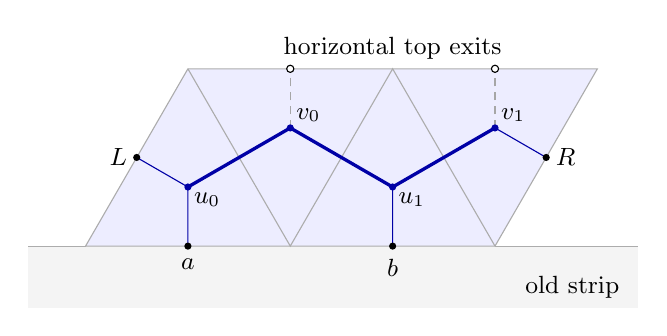
\begin{tikzpicture}[x=2.6cm,y=2.6cm,font=\small]
 \def\d{0.8660254038}
 \fill[gray!9] (-.78,-.30) rectangle (2.20,0);
 \fill[blue!7] (-.5,0)--(1.5,0)--(2,\d)--(0,\d)--cycle;
 \draw[gray!65] (-.5,0)--(1.5,0)--(2,\d)--(0,\d)--cycle;
 \draw[gray!65] (0,\d)--(.5,0)--(1,\d)--(1.5,0);
 \draw[gray!65] (-.78,0)--(-.5,0) (1.5,0)--(2.20,0);
 \draw[very thick,blue!65!black]
    (0,{\d/3})--(.5,{2*\d/3})--(1,{\d/3})--(1.5,{2*\d/3});
 \draw[blue!65!black]
    (0,0)--(0,{\d/3})--(-.25,{\d/2})
    (1,0)--(1,{\d/3})
    (1.5,{2*\d/3})--(1.75,{\d/2});
 \draw[densely dashed,gray!70]
    (.5,{2*\d/3})--(.5,\d)
    (1.5,{2*\d/3})--(1.5,\d);
 \foreach \x/\y/\lab in {0/{\d/3}/u_0,.5/{2*\d/3}/v_0,1/{\d/3}/u_1,1.5/{2*\d/3}/v_1}{
    \fill[blue!65!black] (\x,\y) circle (1.3pt);
 }
 \node[below right,inner sep=2pt] at (0,{\d/3}) {$u_0$};
 \node[above right,inner sep=2pt] at (.5,{2*\d/3}) {$v_0$};
 \node[below right,inner sep=2pt] at (1,{\d/3}) {$u_1$};
 \node[above right,inner sep=2pt] at (1.5,{2*\d/3}) {$v_1$};
 \foreach \x/\lab in {0/a,1/b}{
    \fill (\x,0) circle (1.3pt);
    \node[below] at (\x,-.015) {$\lab$};
 }
 \fill (-.25,{\d/2}) circle (1.3pt);
 \fill (1.75,{\d/2}) circle (1.3pt);
 \node[left] at (-.25,{\d/2}) {$L$};
 \node[right] at (1.75,{\d/2}) {$R$};
 \draw[fill=white] (.5,\d) circle (1.3pt) (1.5,\d) circle (1.3pt);
 \node[above] at (1,\d) {horizontal top exits};
 \node[anchor=west] at (1.60,-.20) {old strip};
\end{tikzpicture}
\caption{The exact two-rhombus addition for the kernel variation.
The four blue vertices are triangle centers; $a,b$ are the old top
ports. A path to $L$ or $R$ enters this chain through exactly one of
$a,b$. The dashed half-edges lead to horizontal exits, whose imaginary
contributions vanish.}
\label{fig:08-kernel-bump}
\end{figure}

A path to $L$ or $R$ crosses the two-port interface an odd number of
times, hence exactly once. The four possible continuations have weights
\[
\begin{array}{c|cc}
 & L & R\\ \hline
 a & \rho & \rho^4\\
 b & \rho^3 & \rho^2
\end{array}
\]
according to the number of new vertices they visit. Thus their combined
contribution to the imaginary identity is
\[
 \sin\lambda\bigl(\rho b_h(x)+\rho^3b_h(x+1)\bigr)
 -\sin(2\lambda)\bigl(\rho^4b_h(x)+\rho^2b_h(x+1)\bigr).
\]
Using $\sin\lambda\,\rho=\sin(2\lambda)\rho^2$, this equals
\[
 \sin\lambda\,\rho(1-\rho^2)
       \bigl(b_h(x)-b_h(x+1)\bigr).
\]
There can be no other occupied segment in the raised part: another visit
would require at least three interface crossings, while its horizontal
top ports are vacant for a path ending at a step exit.

Subtract the old imaginary winding identity. The absolute value of the
remaining bottom contribution is bounded by a constant times the mass of
new arches using the bump. For distinct bump positions these arch families
are disjoint: a member enters and leaves the last band through that specific
adjacent pair, and uses no other port there. Their sum is bounded by
\(A_{h+1}-A_h\). The real strip identity
\(\cos(3\lambda)A_h+B_h=1\), with \(\lambda=\pi/8\), gives
the assertion. To justify the infinite-strip identities, first fix a finite set of
bump positions and perform each calculation in a wide finite
parallelogram. Lemma~\ref{lem:08-localization} bounds every side-error
mass by \(C_h M^{-5/4}\), which tends to zero as the lateral cutoff
\(M\) increases with \(h\) fixed. After this limit, increase the finite
set of bump positions. The nonnegative, disjoint new-arch masses sum
monotonically to at most \(A_{h+1}-A_h\), whose
finiteness is part of Theorem~\ref{thm:01-strip}.
\end{proof}

A \emph{seam} is a lattice line with a specified crossing property that
allows the pieces of a sewn path to be recovered. There is no tangency
convention to choose: a visited internal port is traversed normally, and
crossing a lattice line means traversing such a port. A line crossed once
splits a bridge into two bridges. A line crossed twice, with both endpoints
on its near side, cuts off one arch excursion. Excursions beyond ordered
lines of the latter kind are nested.

\begin{lemma}[Seam moment bounds]
\label{lem:08-seam-moments}
Let $\mathcal F$ be a family of port paths, and let $N(\gamma)$ count
specified seams in an interval of $R$ parallel lattice levels. They are
either once-crossed levels, or twice-crossed levels with both endpoints
on their near side; in the latter case the excursions beyond the counted
levels are nested. Suppose that, after cutting at any ordered list of
such seams, the end pieces have bounded strip or convex boundary sums
when summed successively from their cut ports. Allow a factor $R_0^C$
for source and placement choices, where $C$ is independent of the number
of selected seams and $R\le C_0R_0$.
Then, for every fixed positive integer $j$, the weighted count over
$\mathcal F$ satisfies
\[
 \sum_\gamma\rho^{|\gamma|}N(\gamma)^j
 \le R_0^C C_j
 \begin{cases}
 R^{1+3(j-1)/4},&\text{one crossing},\\
 R^{1+(j-1)/2},&\text{one arch excursion}.
 \end{cases}
\]
Consequently counts exceeding \(R^{3/4}R_0^\varepsilon\), respectively
\(R^{1/2}R_0^\varepsilon\), have arbitrarily polynomially small weighted
mass as \(R_0\to\infty\), including after multiplication by any fixed
polynomial in \(R_0\).
\end{lemma}
\begin{proof}
Expand \(N^j\) and order the selected levels, allowing repetitions. Each
internal gap \(g\) requires one bridge in the first case and two in the
second. Removing mutual avoidance can only increase the resulting upper
bound. The gap factors are therefore at most
\(C(1+g)^{-1/4}\) and \(C(1+g)^{-1/2}\), respectively. Summing the
first level in \(R\) ways and each following gap gives the displayed
bounds, with the ordering and repetitions absorbed in \(C_j\).
For a threshold \(Q\), use
\[
 \sum\rho^{|\gamma|}N^a\mathbf1_{\{N>Q\}}
 \le Q^{-(j-a)}\sum\rho^{|\gamma|}N^j
\]
for a fixed \(a\) and then choose \(j\) sufficiently large. All paths in
a box of diameter \(O(R_0)\) have length \(O(R_0^2)\), so length powers
and raw geometric multiplicities can be included in the polynomial factor.
\end{proof}

This is a statement about an unnormalized weighted measure. Each subsequent
use specifies the end pieces; no probability estimate is inferred merely
by calling a sewing level typical. For a nonnegative representation count
\(F\), we also use the elementary weighted Cauchy--Schwarz inequality
\[
 \sum_{F>0}\rho^{|\gamma|}
 \ge\frac{\bigl(\sum\rho^{|\gamma|}F\bigr)^2}
           {\sum\rho^{|\gamma|}F^2}.
\]

We will also use the two-crossing argument for polygons of bounded
diameter, modulo translation. Choose an extreme counted line and one
crossing port, including these polynomially many choices in the placement
factor. Cutting there makes two port arches. The outer arch has bounded
strip mass, while further counted lines in the other arch produce the
pairs of bridge gaps above. This reduces the polygon count to the same
path calculation without introducing an unrestricted root sum.

\subsection{Prescribed and free endpoints in narrow tubes}

\begin{lemma}[Fixed endpoints in thin tubes]
\label{lem:08-fixed-tube}
There is \(v>0\) such that, for every fixed \(\delta>0\), every attainable
endpoint displacement \(|x|\le vh\) has bridge mass at least
\(h^{-5/4-o(1)}\) in a tube of transverse radius \(\delta h\) about its
straight join. The estimate is uniform in the endpoint and large \(h\).
\end{lemma}
\begin{proof}
We first allow a sufficiently large fixed tube radius. Let \(H\) be even,
choose \(|k-H/4|\le H/40\), and write \(l=H/2-k\).
Lemma~\ref{lem:08-variation}, summed over these heights, implies that a
positive fraction of the choices have both kernel variations at most
\(C H^{-5/4}\). Their suprema have the same bound, since each summable
kernel tends to zero at infinity. Reflection gives \(b_k(x)=b_k(-x)\),
and likewise for \(l\).

For either good kernel \(f\), localization leaves mass \(\ge cH^{-1/4}\)
on \(O(H)\) endpoint positions. Thus
\(\sum f(x)^2\ge cH^{-3/2}\). Moreover
\[
 \left|\sum_x f(x)f(x+t)-\sum_x f(x)^2\right|
 \le \|f\|_\infty\,\|f(\cdot+t)-f\|_1
 \le C|t|H^{-5/2}.
\]
For \(|t|\le v_0H\), with \(v_0>0\) sufficiently small, the
correlation is at least \(c'H^{-3/2}\). Symmetry turns this into the same
lower bound for the self-convolution. If both constituent bridges are
confined to a lateral box of radius \(DH\), the convolution loss is at
most twice their lost mass times \(\|f\|_\infty\), hence at most
\(CD^{-5/4}H^{-3/2}\). Fix \(D\) large enough.

Concatenate bridges of successive heights \(k,k,l,l\). Convolving the
two pair bounds over \(\asymp H\) intermediate displacements gives mass
\(\ge cH^{-2}\) to each prescribed \(|x|\le v_0H/2\), for every good
\(k\), inside a fixed large tube. Let \(F_*\) count admissible indices
\(k\) for which all three levels \(k,2k,H/2+k\) are crossed once.
Then
\[
 \sum_{\gamma\text{ bridge of height }H}
       \rho^{|\gamma|}F_*(\gamma)^j
       \le C_j H^{(j-1)/4}.
\]
To verify this stronger version of the seam bound, order the chosen
indices. Their levels lie in three disjoint macroscopic bands. A gap
between successive indices creates three bridge gaps, with combined
factor \((1+g)^{-3/4}\). The four outer and interband gaps all have
height \(\asymp H\), contributing \(H^{-1}\). Thus the level sum is
\(H^{-1}H H^{(j-1)/4}\), as asserted, also when some indices coincide.
The sum over good \(k\) of representations of a fixed endpoint has mass
\(\ge cH^{-1}\). By the high moment bound its part with
\(F_*>H^{1/4+\varepsilon}\) is negligible compared with \(H^{-1}\).
Dividing the remaining representation mass by this threshold gives
\(H^{-5/4-\varepsilon}\). An odd height is handled by appending a
one-band bridge of fixed allowable displacement and positive weight;
retain slack in the permitted slope.

We finish with the quantitative iteration. Suppose the endpoint estimate, with arbitrary exponent slack, holds at radius $D_jh$ and all slopes at most $v_j$. Set $D_{j+1}=3D_j/4$. Choose
\[
 0<\eta_j\le\min\left\{\frac1{16},\frac{D_j}{8(1+D_j)},
                         \frac{v_0'2^{-j}}{64}\right\},
 \qquad v_{j+1}=v_j-8\eta_j,
\]
where $v_0'>0$ is the slope range obtained in the preceding construction. Start with $v_0=v_0'$ in this iteration. Since $\sum_{j\ge0}8\eta_j\le v_0'/4$, all $v_j$ remain at least $3v_0'/4$.

Take $|x|\le v_{j+1}h$. Choose a joining level $r$ with $|r-h/2|\le\eta_jh$, and an attainable port $y\in r/2+\Z$ with $|y-xr/h|\le\eta_jh$. There are at least $c_jh^2$ such pairs for all large $h$. The two slopes differ from $x/h$ by at most $3\eta_j$, so both lie in the previously allowed range. The difference between either piece's straight join and the whole join is at most $\eta_jh$. Its tube therefore lies within distance
\[
 D_j(1/2+\eta_j)h+\eta_jh\le(3D_j/4)h
\]
of the whole join. The second displacement is compatible because $x-y\in(h-r)/2+\Z$.

For any $\tau>0$, the product of the two endpoint mass bounds is at least $c_{j,\tau}h^{-5/2-2\tau}$. After summing over the joining choices, representation mass is at least $c_{j,\tau}h^{-1/2-2\tau}$. A representation is recovered from its joining seam alone: that seam determines the joining port and both pieces. Its multiplicity is thus bounded by the count $N$ of once-crossed joining levels. Lemma~\ref{lem:08-seam-moments}, with $a=1$, removes the part where $N>h^{3/4+\tau}$ at a cost smaller than any prescribed negative power of $h$. Dividing the retained representation mass by this threshold gives
\[
 c'_{j,\tau}h^{-5/4-3\tau}.
\]
As $\tau$ is arbitrary, this proves the endpoint estimate at radius $D_{j+1}$ with arbitrary exponent slack. Each step uses finitely many previous constants; they may depend on $j$.

For fixed $\delta>0$, a finite number of steps gives $D_j\le\delta$. The uniform lower bound on all $v_j$ permits a single choice, for example $v=v_0'/2$, for every $\delta$. Choose the exponent slacks successively small enough for the desired final $\varepsilon$. This proves the assertion.
\end{proof}

\begin{lemma}[Free endpoints and widening clearance]
\label{lem:08-free-tube}
For each \(\delta>0\) there are \(c,P>0\) such that a height \(h\)
bridge, with free terminal port, has mass at least
\[
 c h^{-1/4}(s/h)^P
\]
under the requirement that its lateral deviation at height \(y\) is at
most \(\delta(s+y)\), whenever \(s\le h\) exceeds a fixed threshold.
Heights along an edge may be interpolated. In particular a fixed-proportion
tube about the starting normal has mass at least \(c_\delta h^{-1/4}\).
\end{lemma}
\begin{proof}
First construct bridges in a large fixed box with terminal displacement
\(|x|\le v'h\), where \(v'>0\) can be any fixed small number. Use the
four-piece construction above without restricting to good heights.
The localized kernels can be chosen symmetric and retain mass
\(\ge ch^{-1/4}\). Partition their \(O(h)\) endpoint positions into
intervals of width a small multiple of \(v'h\). Pair an interval with its
reflection. Cauchy--Schwarz on the finitely many interval masses shows
that an equal-height pair with small total displacement has mass
\(\ge c(v')h^{-1/2}\). The two pairs therefore give
\(ch^{-1}\) per \(k\), and their representation mass summed over
\(\asymp h\) indices is bounded below by a positive constant. The
previous estimate \(\sum\rho^{|\gamma|}F_*^2\le Ch^{1/4}\) and
weighted Cauchy--Schwarz give mass \(\ge ch^{-1/4}\). Odd heights again
cost only a fixed factor.

For a tube of radius \(\delta h\), divide the height into a sufficiently
large fixed number \(m\) of pieces. Vary the \(m-1\) joining levels in
disjoint small macroscopic intervals near equal division. Apply the
large-box construction to each piece, taking its permitted terminal
slope sufficiently small that cumulative endpoint shifts remain below
\(\delta h/2\), and then \(m\) sufficiently large that each piece's
box fits the remaining clearance. The representation mass is at least
\[
 c_m h^{-1/4}h^{3(m-1)/4}.
\]
The representation count is bounded by the product of the seam counts
in the \(m-1\) intervals. Its second moment is at most
\[
 C_m h^{-1/4}h^{3(m-1)/2}.
\]
Indeed in each interval the two selected levels introduce one bridge gap,
whose ordered sum is \(O(h^{7/4})\), while the \(m\) other gaps are
macroscopic and contribute \(h^{-m/4}\). Cauchy--Schwarz proves the
fixed-proportion tube assertion.

For the widening tube use seam intervals
\([r_i,5r_i/4]\), where \(r_i=4^is\), stopping before \(h/2\).
The proportional width for each piece is chosen small enough that the
geometric sum of all previous endpoint shifts and current fluctuations
is at most \(\delta(s+y)\). If there are no intervals, one
fixed-proportion tube suffices. With \(k\) intervals the representation
mass and second moment are bounded respectively below and above by
\[
 c^{k+1}h^{-1/4}\prod_i r_i^{3/4},\qquad
 C^{k+1}h^{-1/4}\prod_i r_i^{3/2}.
\]
The moment estimate follows by selecting two seams in each interval:
its gap factor sums to \(O(r_i^{7/4})\), and the outer gaps contribute
\(h^{-1/4}\prod_i r_i^{-1/4}\). Constants are uniform in the number
of intervals because the scales are separated by four. Thus
Cauchy--Schwarz leaves \((c^2/C)^{k+1}h^{-1/4}\).
Since \(k=O(1+\log(h/s))\), this is the asserted bound for some fixed
finite \(P\).
\end{proof}

Figure~\ref{fig:08-tubes} contrasts the prescribed and free terminal
constraints in the two tube estimates.

\begin{figure}[tb]
\centering
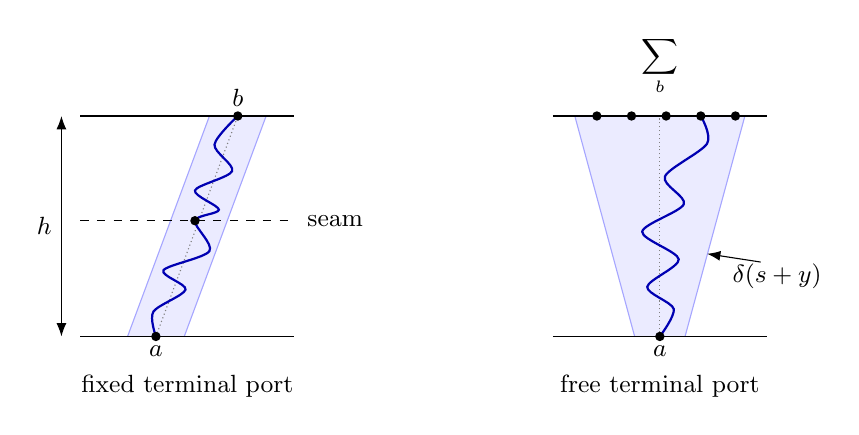
\begin{tikzpicture}[x=0.8cm,y=0.7cm,>=Latex,font=\small]
 \begin{scope}
  \fill[blue!8] (-0.45,0)--(0.45,0)--(1.75,4)--(0.85,4)--cycle;
  \draw[blue!35] (-0.45,0)--(0.85,4) (0.45,0)--(1.75,4);
  \draw (-1.2,0)--(2.2,0) (-1.2,4)--(2.2,4);
  \draw[densely dotted,gray] (0,0)--(1.3,4);
  \draw[dashed] (-1.2,2.1)--(2.2,2.1);
  \draw[blue!70!black,thick]
   plot[smooth] coordinates {(0,0) (-0.04,0.45) (0.47,0.85)
   (0.12,1.2) (0.85,1.55) (0.62,2.1) (1,2.3) (0.62,2.65)
   (1.21,3) (0.93,3.48) (1.3,4)};
  \fill (0,0) circle (1.7pt) node[below] {$a$};
  \fill (1.3,4) circle (1.7pt) node[above] {$b$};
  \fill (0.62,2.1) circle (1.7pt);
  \node[anchor=west] at (2.25,2.1) {seam};
  \draw[<->] (-1.5,0)--node[left] {$h$}(-1.5,4);
  \node at (0.5,-0.9) {fixed terminal port};
 \end{scope}
 \begin{scope}[xshift=6.4cm]
  \fill[blue!8] (-0.4,0)--(0.4,0)--(1.35,4)--(-1.35,4)--cycle;
  \draw[blue!35] (-0.4,0)--(-1.35,4) (0.4,0)--(1.35,4);
  \draw (-1.7,0)--(1.7,0) (-1.7,4)--(1.7,4);
  \draw[densely dotted,gray] (0,0)--(0,4);
  \draw[blue!70!black,thick]
   plot[smooth] coordinates {(0,0) (0.22,0.5) (-0.2,0.9)
   (0.3,1.4) (-0.28,1.9) (0.38,2.4) (0.08,2.9)
   (0.75,3.5) (0.65,4)};
  \fill (0,0) circle (1.7pt) node[below] {$a$};
  \foreach \x in {-1,-0.45,0.1,0.65,1.2}
   \fill (\x,4) circle (1.7pt);
  \node[above] at (0,4.2) {$\displaystyle\sum_b$};
  \node at (0,-0.9) {free terminal port};
  \node[anchor=west] at (1.0,1.1) {$\delta(s+y)$};
  \draw[->] (1.6,1.35)--(0.75,1.5);
 \end{scope}
\end{tikzpicture}
\caption{Schematic tube constraints. Left: a fixed endpoint contribution;
the once-crossed seam recovers both pieces and their common port. Right:
a widening tube with terminal ports summed over. Shading denotes spatial
confinement; both lemmas bound unnormalized path mass.}
\label{fig:08-tubes}
\end{figure}

\subsection{Closing paths and controlling their second length moment}

A bridge crossing mass is not a second length moment. To obtain the latter, we close each path by an exterior path of controlled positive mass and compare with the polygon second moment. The closing line must remain recoverable: its multiplicity is the source of the extra exponents below.

\begin{lemma}[Localized arch kernel]
\label{lem:08-arch-kernel}
Two distinct ports on a lattice side line, at distance \(r\), can be joined in either
prescribed half-plane by arches of diameter at most \(Cr\), of total
mass at least \(r^{-5/4-o(1)}\).
\end{lemma}
\begin{proof}
There are constants \(0<a<b<\infty\) such that height \(h\) arches,
localized to a fixed box of size \(h\), have rightward displacement in
\([ah,bh]\) with mass at least \(ch^{-1/4}\). To see this, start from
\(\sum_{s>0}sK_h(s)\asymp h^{3/4}\). Localization and dyadic summation
bound the first moment at displacements above \(bh\) by
\(Ch(bh)^{-1/4}\). For \(1\le q\le h\), arches of displacement at
least \(q\) have total mass \(O(q^{-1/4})\): those leaving the
height-\(\lfloor q\rfloor\) strip cost \(O(B_{\lfloor q\rfloor})\)
by the strip winding identity, and those remaining have this bound by
the first displacement moment in that smaller strip. Integrating this
tail up to \(ah\) bounds its first moment by \(O((ah)^{3/4})\).
Choose \(a\) small and \(b\) large. Finally, removal of paths leaving a
sufficiently wide box changes the first moment on \([ah,bh]\) by an
arbitrarily small multiple of \(h^{3/4}\), by
Lemma~\ref{lem:08-localization}. Division by \(bh\) proves the claim.

From the prescribed ports run two bridges into the chosen half-plane to
a line at height \(k\in[Dr,2Dr]\), with \(D\) a large fixed constant.
Join their terminal ports by one of the just-constructed arches beyond
that line, of height \(r\) and displacement in \([ar,br]\).
There are \(\asymp r\) translations of this arch in a small macroscopic
interval near the starting ports. For each translation and arch endpoint
separation, use Lemma~\ref{lem:08-fixed-tube} for both bridges. Choose
\(D\) large enough for their slopes and their tube widths small enough
that they are disjoint. This is possible because the two straight segments
remain in the same order and their separation is at least
\(\min(1,a)r\). Translation along the terminal line preserves the port
parities. For each \(k\) the product mass is therefore at least
\(r\,r^{-5/2-o(1)}r^{-1/4}=r^{-7/4-o(1)}\).

Summing \(k\) gives representation mass \(r^{-3/4-o(1)}\). A
representation is recovered at its two-crossing seam. The end pieces are
two bridges from the prescribed ports, the internal gaps require two
bridges each, and the last piece is an arch; all their endpoint sums are
bounded. Lemma~\ref{lem:08-seam-moments} discards multiplicity above
\(r^{1/2+\varepsilon}\), proving the assertion. The construction has
diameter \(O(r)\). The finitely many bounded nonzero distances have
positive weight by fixed ordinary arches and are absorbed in the constants.
\end{proof}

\begin{proposition}[Localized strip second moment]
\label{prop:08-strip-second}
For each fixed \(C_0\), and a fixed starting port,
\begin{equation}
 \sum_{\substack{\gamma\text{ arch or bridge in height }h\\
                  \operatorname{diam}\gamma\le C_0h}}
       \rho^{|\gamma|}|\gamma|^2
       \le h^{29/12+o(1)}.
 \label{eq:R-32a}
\end{equation}
\end{proposition}
\begin{proof}
Figure~\ref{fig:08-exterior-closures} shows the two closures and their
recovery lines. An arch needs one movable line; a bridge needs two lines
that move together at fixed separation. This coupling improves the
bridge's inverse multiplicity and compensates for its more costly closure.
\begin{figure}[tb]
\centering
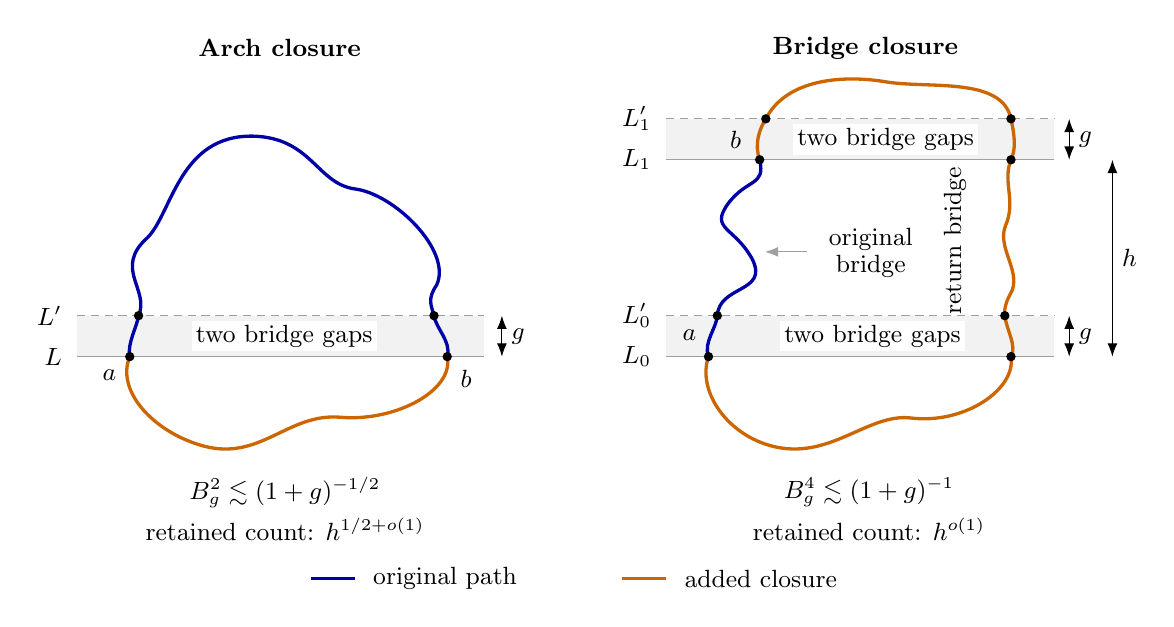
\begin{tikzpicture}[x=1.12cm,y=1cm,>=Latex,font=\small,
  original/.style={blue!65!black,very thick},
  added/.style={orange!80!black,very thick},
  clean/.style={gray!75,thin},
  comparison/.style={gray!75,densely dashed,thin},
  port/.style={circle,fill=black,inner sep=1.2pt}]
  \begin{scope}
    \node at (1.7,3.92) {\textbf{Arch closure}};
    \fill[gray!10] (-.60,0) rectangle (4.02,.52);
    \draw[clean] (-.60,0)--(4.02,0);
    \draw[comparison] (-.60,.52)--(4.02,.52);
    \node[anchor=east] at (-.66,0) {$L$};
    \node[anchor=east] at (-.66,.52) {$L'$};
    \draw[original]
      (0,0) .. controls (-.03,.17) and (.08,.37) .. (.10,.52)
      .. controls (.23,.85) and (-.19,1.12) .. (.20,1.51)
      .. controls (.48,1.82) and (.56,2.82) .. (1.40,2.80)
      .. controls (2.06,2.78) and (2.12,2.20) .. (2.55,2.13)
      .. controls (3.00,2.07) and (3.66,1.34) .. (3.48,.91)
      .. controls (3.37,.73) and (3.42,.65) .. (3.45,.52)
      .. controls (3.47,.36) and (3.65,.19) .. (3.60,0);
    \draw[added]
      (3.60,0) .. controls (3.68,-.43) and (3.01,-.83) .. (2.39,-.77)
      .. controls (1.78,-.71) and (1.47,-1.36) .. (.79,-1.12)
      .. controls (.26,-.94) and (-.16,-.43) .. (0,0);
    \node[port,label=below left:$a$] at (0,0) {};
    \node[port,label=below right:$b$] at (3.60,0) {};
    \node[port] at (.10,.52) {};
    \node[port] at (3.45,.52) {};
    \node[fill=white,inner sep=1.5pt] at (1.75,.26) {two bridge gaps};
    \draw[<->] (4.22,0)--node[right] {$g$}(4.22,.52);
    \node at (1.76,-1.72) {$B_g^2\lesssim(1+g)^{-1/2}$};
    \node at (1.76,-2.19) {retained count: $h^{1/2+o(1)}$};
  \end{scope}
  \begin{scope}[xshift=7.35cm]
    \node at (1.78,3.92) {\textbf{Bridge closure}};
    \fill[gray!10] (-.48,0) rectangle (3.92,.52);
    \fill[gray!10] (-.48,2.50) rectangle (3.92,3.02);
    \draw[clean] (-.48,0)--(3.92,0);
    \draw[clean] (-.48,2.50)--(3.92,2.50);
    \draw[comparison] (-.48,.52)--(3.92,.52);
    \draw[comparison] (-.48,3.02)--(3.92,3.02);
    \node[anchor=east] at (-.54,0) {$L_0$};
    \node[anchor=east] at (-.54,.52) {$L'_0$};
    \node[anchor=east] at (-.54,2.50) {$L_1$};
    \node[anchor=east] at (-.54,3.02) {$L'_1$};
    \draw[original]
      (0,0) .. controls (-.06,.18) and (.09,.36) .. (.10,.52)
      .. controls (.12,.91) and (.68,.81) .. (.50,1.23)
      .. controls (.30,1.65) and (.01,1.61) .. (.22,1.94)
      .. controls (.44,2.27) and (.65,2.16) .. (.58,2.50);
    \draw[added]
      (.58,2.50) .. controls (.52,2.69) and (.57,2.88) .. (.65,3.02)
      .. controls (.90,3.56) and (1.59,3.57) .. (2.01,3.49)
      .. controls (2.49,3.40) and (3.33,3.56) .. (3.43,3.02)
      .. controls (3.47,2.81) and (3.49,2.64) .. (3.43,2.50);
    \draw[added]
      (3.43,2.50) .. controls (3.33,2.22) and (3.49,1.98) .. (3.37,1.67)
      .. controls (3.26,1.38) and (3.57,1.06) .. (3.42,.79)
      .. controls (3.37,.69) and (3.35,.59) .. (3.36,.52)
      .. controls (3.38,.33) and (3.50,.14) .. (3.43,0);
    \draw[added]
      (3.43,0) .. controls (3.49,-.41) and (2.91,-.86) .. (2.30,-.78)
      .. controls (1.80,-.71) and (1.37,-1.34) .. (.70,-1.13)
      .. controls (.19,-.97) and (-.13,-.42) .. (0,0);
    \foreach \x/\y in {0/0,.58/2.50,3.43/2.50,3.43/0,
                        .10/.52,3.36/.52,.65/3.02,3.43/3.02}
      \node[port] at (\x,\y) {};
    \node[anchor=south east] at (-.03,.08) {$a$};
    \node[anchor=south east] at (.48,2.52) {$b$};
    \node[fill=white,inner sep=1.5pt] at (1.86,.26) {two bridge gaps};
    \node[fill=white,inner sep=1.5pt] at (2.01,2.76) {two bridge gaps};
    \draw[<->] (4.09,0)--node[right] {$g$}(4.09,.52);
    \draw[<->] (4.09,2.50)--node[right] {$g$}(4.09,3.02);
    \draw[<->] (4.58,0)--node[right] {$h$}(4.58,2.50);
    \node[align=center] at (1.84,1.32) {original\\[-1pt]bridge};
    \draw[->,gray!75] (1.12,1.33)--(.64,1.33);
    \node[rotate=90,anchor=south] at (3.03,1.47) {return bridge};
    \node at (1.82,-1.72) {$B_g^4\lesssim(1+g)^{-1}$};
    \node at (1.82,-2.19) {retained count: $h^{o(1)}$};
  \end{scope}
  \draw[original] (2.05,-2.82)--(2.55,-2.82);
  \node[anchor=west] at (2.65,-2.82) {original path};
  \draw[added] (5.58,-2.82)--(6.08,-2.82);
  \node[anchor=west] at (6.18,-2.82) {added closure};
\end{tikzpicture}
\caption{Closure and recovery in Proposition~\ref{prop:08-strip-second}.
Modulo translation, solid lines recover the original path up to bounded
choices; dashed lines illustrate a second admissible placement. Left: moving the clean
line creates two bridge gaps. Right: move the lower and upper lines
together, keeping their separation $h$. Within a lower-line interval
of width at most $h/3$, the two comparison bands are disjoint and create
four bridge gaps. Their gap factors sum as a power and a logarithm,
respectively, giving the displayed counts after discarding the weighted
high-multiplicity exceptions. Curves are schematic; no intermediate
line is required to be clean.}
\label{fig:08-exterior-closures}
\end{figure}


Close an arch by an exterior arch supplied by
Lemma~\ref{lem:08-arch-kernel}, at mass at least
\(h^{-5/4-o(1)}\). The result is a simple polygon of diameter \(O(h)\),
and its original boundary is a two-crossing seam. Modulo translation,
fixing this line recovers the two arcs and the input start up to bounded
choices. Its placement count has moments at most \(C_jh^{C+j/2}\),
with \(C\) independent of \(j\): choose an initial line and crossing
port in polynomially many ways, order the other levels, use two bridges
per internal gap and bounded terminal arch sums. Thus multiplicities
above \(h^{1/2+\varepsilon}\) have negligible mass, even with squared
length and raw multiplicity included. The polygon second moment gives
\(h^{5/4+1/2+2/3+o(1)}=h^{29/12+o(1)}\).

For a bridge, attach exterior arches at its bottom and top, ending far
to one common side of the original path. Each new endpoint ranges over
\(ch\) positions at distance \(\asymp h\), with their intervals chosen
so that their mutual displacement satisfies the slope condition of
Lemma~\ref{lem:08-fixed-tube}. Join them by a thin bridge inside the
original strip, separated from the original path. The three added kernels
and two endpoint sums have total mass at least
\(h^2h^{-15/4-o(1)}=h^{-7/4-o(1)}\).

Now there are two clean two-crossing lines at a fixed separation \(h\).
Their joint placement count on the polygon has moments at most
\(C_jh^C(1+\log h)^j\). Indeed restrict the lower line to an interval of
width at most \(h/3\); only boundedly many intervals are needed after
anchoring a polygon of diameter \(O(h)\). Each successive gap \(g\)
then forces two bridges in the lower band and two in the upper, giving
\((1+g)^{-1}\); its sum is \(O(1+\log h)\). The excursions are nested
and all remaining pieces have bounded strip sums, with only polynomial
placement costs. For fixed lines the two bridges and exterior arches are
recovered up to bounded orientation choices. High moments therefore
discard multiplicity above \(h^\varepsilon\). The polygon estimate now
gives \(h^{7/4+2/3+o(1)}=h^{29/12+o(1)}\).
In both cases the input length is at most the polygon length. Exceptional
representation mass is harmless because every path stays in an \(O(h)\)
box and hence has length \(O(h^2)\).
\end{proof}

\subsection{Transferring bulk length to bridges}

Let \(D\) be a lattice equilateral triangle of side \(H\), and let
\(\mathcal C_H\) be its boundary-to-boundary chords which visit a fixed
central subtriangle at positive proportional distance from \(\partial D\).
Ordered endpoints or boundedly many port types change only constants.
Lemma~\ref{lem:08-localization}, applied at each of the \(O(H)\)
boundary sources, gives
\[
 \sum_{\gamma\in\mathcal C_H}\rho^{|\gamma|}\le CH^{3/4}.
\]
For each of \(\asymp H^2\) internal ports in a smaller central triangle,
the bulk identity bounds \(L_p(D)\) below by a constant times
\(P_2(c_0H)=H^{1/12+o(1)}\), using nests about its neighboring face
centers. Summing over these ports and dropping the cosine yields
\[
 \sum_{\gamma\in\mathcal C_H}\rho^{|\gamma|}|\gamma|
       \ge H^{25/12-o(1)}.
\]

\begin{lemma}[Separation of useful chord endpoints]
\label{lem:08-endpoint-separation}
For every fixed \(\eta>0\), the preceding first-length lower bound
persists after retaining only chords with the following property: endpoints
on the same side have separation at least \(H^{1-\eta}\); endpoints on
distinct sides have maximum distance from their common corner at least
\(H^{1-\eta}\).
\end{lemma}
\begin{proof}
Group the excluded chords by dyadic endpoint scale \(s\), taking
\(s\asymp1\) for bounded separations. For a common side, fix a source
and close outside \(D\) with an arch of mass
\(s^{-5/4-o(1)}\). The two-crossing seam argument in
Proposition~\ref{prop:08-strip-second}, now using diameter \(O(H)\),
gives the squared-length bound, summed over sources,
\[
 \sum_{\substack{\gamma\text{ with same-side endpoints}\\
                  \text{at scale }s}}
       \rho^{|\gamma|}|\gamma|^2
       \le H^{1+2/3+1/2+o(1)}s^{5/4}.
\]
The factor \(H\) counts sources; the factor \(H^{1/2+o(1)}\) bounds
seam multiplicity. All small exponent losses can be assigned to \(H\).
For distinct sides we claim
\begin{equation}
 \sum_{\substack{\gamma\text{ with distinct-side endpoints}\\
                  \text{at corner scale }s}}
       \rho^{|\gamma|}|\gamma|^2
       \le H^{2/3+o(1)}s^{11/4}.
 \label{eq:R-32b}
\end{equation}
Here the sum includes every source and endpoint pair at that scale.

By symmetry put the sides at
\[
 A:\ y=0,\qquad B:\ x=y/\sqrt3,
\]
with \(D\) above \(A\) and to the right of \(B\). Write the endpoints
as \(a\in A,b\in B\), choosing \(b\) farther from the shared corner.
Then \(y_b\asymp s\). Put \(w=y/2-d_0x\); the half-plane exterior
to \(B\) is \(w>0\). We first construct a closing arc outside \(D\)
with mass \(s^{-3/2-o(1)}\) and diameter \(O(s)\).
Join \(a\), below \(A\), to a port \((X,0)\) with
\(X\in[-8s,-7s]\). The arch kernel costs \(s^{-5/4-o(1)}\).
We next construct a join from \((X,0)\) to \(b\), within
\(y>0,w>0\), at cost \(s^{-5/4-o(1)}\). Summing over the
\(\asymp s\) choices of \(X\) then gives the required closing mass.

For this two-face join choose small fixed \(\alpha>0\). From \(b\)
first reach a horizontal line \(y=t\), where
\(t-y_b\in[\alpha s,2\alpha s]\). The comparison domain lies between
\(B\) and a parallel line at \(w\)-depth approximately \(10\alpha s\),
with the additional inequalities
\[
 y\ge0,\qquad
 x\le x_b+(\alpha/4)s-(y-y_b)/\sqrt3.
\]
A thin bridge tube in the inward normal direction \((-d_0,1/2)\)
from \(B\) to the far parallel line fits these inequalities and passes
beyond \(y=t\). Its mass is \(\ge cs^{-1/4}\) by
Lemma~\ref{lem:08-free-tube}. Convex cut comparison gives the same lower
bound for exits on \(y=t\). Every such exit \(z\) satisfies
\(w(z)\ge c\alpha s\), by the oblique upper bound on \(x\).
The lower bound on \(x\), from \(y\ge0,w=O(\alpha s)\), keeps all
these paths well to the right of \(X\).

Continue from \(z\) vertically to \(y=L\), where
\(L\in[D_2s,2D_2s]\) and \(D_2\) is a large fixed constant. A tube
of width a sufficiently small multiple of \(s\) stays clear of \(B\)
and of the future arm from \(X\); its mass is
\(\ge c_{D_2}s^{-1/4}\). For each \(t\) the product mass is therefore
\(\ge c_{D_2}s^{-1/2}\). Sum over \(\asymp s\) choices of \(t\).
Each is recovered as a once-crossed seam. The initial segment has bounded
convex-boundary mass in the two-face wedge with distant walls, the final
segment has bounded strip mass, and internal gaps are bridges.
Lemma~\ref{lem:08-seam-moments} discards counts above
\(s^{3/4+\varepsilon}\). Thus the distinct \(b\)-arms to \(L\) have
mass at least \(s^{-1/4-o(1)}\).

Independently take a vertical arm from \((X,0)\) to \(L\) in a disjoint
small-width tube, with mass \(\ge cs^{-1/4}\). Connect the two new ports
by an arch beyond \(L\) of mass \(s^{-5/4-o(1)}\). Their lateral
separation is \(O(s)\) independently of \(D_2\); hence the arch diameter
constant is independent of \(D_2\), and increasing \(D_2\) makes this
arch lie wholly in \(w>0\). Vary \(L\) over its interval. These are
exactly two-crossing seams; the two initial arms have bounded convex
boundary sums, the intermediate gaps give pairs of bridges, and the
terminal arch has bounded mass. Removing multiplicity above
\(s^{1/2+\varepsilon}\) gives
\[
 s\,s^{-1/4-o(1)}s^{-1/4}s^{-5/4-o(1)}
       /s^{1/2+\varepsilon}=s^{-5/4-o(1)}
\]
for the two-face join. All walls and cuts are lattice lines rounded with
proportional slack; distant walls can be added to make every comparison
domain finite. For bounded scales, first move \(b\) a fixed number of
bands into \(w>0\) by elementary bridges with displacement
\((-1/2,d_0)\), which remain in \(y>0\). Perform the construction from
that translated parallel boundary. Keep the auxiliary interval on
$y=0$, shifting it tangentially relative to the new boundary's
intersection with $y=0$. This costs a positive constant and preserves the
required original-side crossings.

We now count inverse images of the resulting polygon. It crosses \(A\)
exactly twice, and its arc above \(A\) crosses \(B\) exactly once;
other crossings of \(B\) do not matter. Given both lines, these properties
recover the original chord and closing arc up to bounded choices. Each
line position is within \(O(s)\) levels of the corresponding directional
extremum of the polygon. For \(A\), the two-crossing moment bound gives
at most \(s^{1/2}H^\varepsilon\) choices, outside negligible weighted
exceptions. For each \(A\), apply the one-crossing moment bound to its
positive-side arc to obtain at most \(s^{3/4}H^\varepsilon\) choices
of \(B\). To justify the end factors in this second application, retain
the \(A\) half-plane and the relevant extreme \(B\) half-plane for
each end piece, with distant walls. Convex winding bounds its boundary
sum; the opposite \(A\)-arc has bounded arch mass. Initial roots,
outermost levels, and the union over \(A\) cost only a fixed polynomial
in \(H\), independent of the moment order. Thus the total inverse
multiplicity is at most \(s^{5/4}H^{2\varepsilon}\). Two nonparallel
lines determine the placement of the fixed triangle. Squared lengths and
all discarded raw multiplicities are polynomial in \(H\), so their
exceptional contribution is negligible. Dividing the polygon second
moment by the added mass \(s^{-3/2-o(1)}\) proves
\eqref{eq:R-32b}.

Finally apply Cauchy--Schwarz with the central-visit mass \(CH^{3/4}\).
The same-side contribution at scale \(s\) is at most
\(H^{35/24+o(1)}s^{5/8}\); the distinct-side contribution is at most
\(H^{17/24+o(1)}s^{11/8}\). At \(s\le CH^{1-\eta}\) these are
respectively at most
\(H^{25/12-5\eta/8+o(1)}\) and
\(H^{25/12-11\eta/8+o(1)}\). Summing the \(O(\log H)\) scales is
power-smaller than the original first-length lower bound.
\end{proof}

\begin{lemma}[Exterior connectors to an outer strip]
\label{lem:08-connectors}
Embed a triangle of side \(H=\lfloor c_0M\rfloor\), for small fixed
\(c_0>0\), in a strip of height \(M\). For each of the endpoint types
in Lemma~\ref{lem:08-endpoint-separation}, choose one of the finitely many
lattice strip orientations. The strip can be placed in \(\asymp M\)
ways with both boundaries at distance at least \(cM\) from \(D\).
At endpoint scale $s$, two disjoint exterior connectors to free ports
on these boundaries have product mass at least
\begin{equation}
 H^{-1/2-o(1)}(s/H)^P,
 \label{eq:R-32c}
\end{equation}
for a finite fixed \(P\). They and \(D\) stay in a box of diameter
\(CM\), with \(C,P\) independent of \(\eta\).
\end{lemma}
\begin{proof}
For distinct sides use the coordinates \(A,B,a,b,w\) from the preceding
proof and a horizontal outer strip. Connect \(a\) to the lower boundary
by a localized bridge below \(A\). For \(b\), take bridges from \(B\)
in direction \((-d_0,1/2)\) to a sufficiently distant parallel line,
so that their straight tubes pass beyond the upper target boundary.
Because \(y_b\asymp s\), the widening tubes of
Lemma~\ref{lem:08-free-tube} with initial clearance \(s\) fit inside
\(y>0,w>0\), on reducing their fixed proportional width. Include these
half-plane constraints and distant bounding walls in a convex comparison
domain. Cut at the upper target line. Lemma~\ref{lem:08-localization}
gives mass \(\ge cH^{-1/4}(s/H)^P\) for the \(b\)-arm; the
\(a\)-arm has mass \(\ge cH^{-1/4}\). The two arms lie on opposite
sides of \(A\), and avoid \(D\). On the resulting bridge, \(A\) is
crossed once and \(B\) is crossed once on the tail following \(A\).

For a common horizontal side \(A\), write \(x_a<x_b\) with separation
\(\asymp s\). Orient the outer strip in crossing direction
\(p=(d_0,-1/2)\). Separate the arms by a lattice wall parallel to
\[
 x=(x_a+x_b)/2+y/\sqrt3.
\]
The separator is a $p$-level, since $p\cdot(x,y)=d_0x-y/2$ is
constant on it. Both arms lie below \(A\), the arm from \(b\) to the upper \(p\)-boundary
on the right of the wall. Construct this arm by taking downward bridges
in direction \(n=(0,-1)\) in a longer convex domain and cutting at the
target \(p\)-line. Since \(n\cdot p=1/2\), they reach that target.
Their widening tubes, with initial scale \(s\), remain right of the
separator and inside the opposite outer strip bound. They give mass
\(\ge cH^{-1/4}(s/H)^P\).

The arm from \(a\) must turn toward the lower outer boundary. Put
\(q=(-d_0,-1/2)\). First reach a \(q\)-normal line at depth in
\([\alpha s,2\alpha s]\) from \(a\), with small fixed \(\alpha>0\).
Writing \(t=-y\), use the convex domain with
\[
 0\le t\le10\alpha s,
 \qquad x\ge x_a-(\alpha/4)s-t/\sqrt3,
\]
also restricted to the left of the separator and to the outer strip where
needed. A thin downward bridge tube fits and passes beyond the chosen
\(q\)-line, so cutting gives mass \(\ge cs^{-1/4}\). Its exits \(z\)
satisfy \(t(z)\ge c\alpha s\) and
\(|x(z)-x_a|=O(\alpha s)\), using
\[
 q\cdot(z-a)=-d_0(x(z)-x_a)+t(z)/2.
\]
From \(z\), continue in positive \(q\) direction in the half-plane beyond
this switching line. A widening tube of initial scale \(s\) remains
below \(A\), left of the separator, and clear of the opposite outer
boundary: its depth below \(A\) and clearance from the separator both
grow linearly along \(q\). Since \(q\cdot(-p)=1/2\), long enough
bridges in this direction cross the lower target line. Convex truncation
there gives mass \(\ge cH^{-1/4}(s/H)^P\).

Sum the switching line over \(\asymp s\) choices. It is recovered as a
once-crossed seam; the extreme end pieces have bounded convex-boundary
mass after retaining the original and target boundaries and the extreme
seam half-planes. The seam moment bound, allowing a polynomial factor in
\(H\), removes counts above \(s^{3/4}H^\varepsilon\). The line count
\(s\) cancels the short-arm factor \(s^{-1/4}\) and this seam factor.
The resulting left arm has mass
\(H^{-1/4-o(1)}(s/H)^P\), proving \eqref{eq:R-32c} after combining
with the right arm and, if necessary, increasing \(P\).
The entire output crosses \(A\) exactly twice, with its endpoints on
its exterior side.

The widening-tube construction above requires $s$ to exceed a fixed
threshold. To include bounded $s$, choose a fixed integer $K$ above that
threshold and first add the following elementary stems. On a common
side, take $K$ downward one-band bridges from $a$, each with displacement
$(-1/2,-d_0)$, and from $b$, each with displacement $(1/2,-d_0)$.
The stems are disjoint, remain respectively in $x\le x_a$ and
$x\ge x_b$, and end on $A'=\{y=-Kd_0\}$ with separation
$(x_b-x_a)+K\asymp s+K$.
Apply the preceding common-side construction below $A'$. The new arms
avoid the stems; the completed output still crosses the original $A$
exactly twice. For distinct
sides, extend $b$ by $K$ elementary $B$-normal bridges of displacement
$(-1/2,d_0)$. Their endpoint $b'$ lies on $B'=\{w=Kd_0\}$ with
$y_{b'}\ge Kd_0$. Run the $b$-arm construction in $y>0,w>Kd_0$.
The new arm avoids the stem, the triangle, and the downward $a$-arm;
the completed $b$-arm retains the required single crossing of the
original $B$. The enlarged scales
are fixed positive constants for bounded $s$, so their powers of $s/H$
are comparable up to constants. The stems have fixed positive weights,
and change all outer-strip clearances by $O(K)$ only.

All comparison domains here are intersections of the specified lattice
half-planes, a starting and a far terminal line normal to the comparison
bridge, and distant lattice walls. The fitted tube stays inside with
proportional slack away from its endpoints. This verifies that every cut
comparison is between convex domains and avoids assuming uniform
continuation weights for individual prefixes. The allowed normal strip
placements form an interval of \(\asymp M\) choices; all distances and
tube diameters are fixed multiples of \(M\).
\end{proof}

\begin{proposition}[A localized bridge length lower bound]
\label{prop:08-localized-length}
For a sufficiently large fixed \(C\), the height \(M\) bridges from a
fixed source and of diameter at most \(CM\) have first-length mass
\(M^{13/12-o(1)}\) in the lower-exponent sense. Consequently, for every
fixed \(\xi>0\), the normalized critical bridge law satisfies
\begin{equation}
 \Prob_M^{\mathrm{br}}\{|\gamma|\ge M^{4/3-\xi}\}\ge M^{-o(1)}.
 \label{eq:R-32d}
\end{equation}
\end{proposition}
\begin{proof}
Fix $0<\eta<1$. Retain the chords from
Lemma~\ref{lem:08-endpoint-separation} and attach the two connectors for
each outer strip placement. Their endpoint scale
obeys \(s\ge H^{1-\eta}\), so the added mass is at least
\(H^{-1/2-P\eta-o(1)}\). Translate every output bridge to a fixed
bottom source. We must count how many inputs yield the same translated
output, including the original placement of \(D\).

For distinct sides, once-crossed \(A\)-levels have at most
\(H^{3/4+\varepsilon}\) choices outside negligible mass. For each such
\(A\), apply the same bound to candidate \(B\)-levels on the specified
tail above \(A\), obtaining another \(H^{3/4+\varepsilon}\). The
initial piece up to \(A\) has a bounded bridge sum. The end pieces for
the \(B\)-counts have bounded convex-boundary mass with the outer strip,
\(A\) half-plane, and relevant extreme \(B\) half-plane retained.
The union over the first level or over \(A\) costs only a polynomial in
\(H\) before taking high moments. These two nonparallel lines determine
\(D\) and the junctions.

For a common side, the permissible \(A\)-levels are crossed twice, with
both output endpoints on the exterior side. Their nested excursions give
at most \(H^{1/2+\varepsilon}\) choices. The end arms lie in the
intersection of the outer strip and the exterior half-plane of the first
level, and the last piece is an arch, so their sequential boundary sums
are bounded. Once the seam and its two crossing ports are fixed, at most
\(O(H)\) tangential placements of \(D\) remain. Thus both endpoint
types have total inverse multiplicity \(H^{3/2+o(1)}\). This also
recovers the outer strip placement by translating back relative to \(D\).
The auxiliary construction parameters within a connector were already
removed in Lemma~\ref{lem:08-connectors}; they are not counted again.
Exceptions remain negligible with length and raw placement factors, since
all output paths lie in an \(O(M)\) box.

The input first-length mass, the \(\asymp M\) outer placements, the
connector mass, and the inverse multiplicity therefore give
\[
 H^{25/12-o(1)}\,cM\,H^{-1/2-P\eta-o(1)}
        /H^{3/2+o(1)}
        =M^{13/12-P\eta-o(1)}.
\]
There are only boundedly many orientations and endpoint orders; apply a
lattice symmetry to the selected class. The width constant is independent
of \(\eta\). Since \(\eta>0\) is arbitrary, this proves the asserted
lower exponent.

For the localized moments defined at the start of the section, we now
have \(m_1\ge M^{13/12-o(1)}\),
\(m_2\le M^{29/12+o(1)}\), and \(m_0\le B_M\asymp M^{-1/4}\).
For \(a=M^{4/3-\xi}\), the first-length mass below \(a\) is at most
\(aB_M=O(M^{13/12-\xi})\), hence negligible. Weighted
Cauchy--Schwarz gives mass at least
\(m_1^2/(4m_2)\ge M^{-1/4-o(1)}\) above the threshold, for large
\(M\). Division by \(B_M\) proves \eqref{eq:R-32d}. This step alone
does not give a high-probability lower bound.
\end{proof}

\FloatBarrier
\subsection{Turning corridors with a free terminal port}

The bridge-length input is now established. The ordered adjacent-path
construction in Section~\ref{sec:10-thermal-probes} also needs paths
that pass an obstacle or turn back to their starting boundary. We prove
that these paths retain free-end mass at least $cH^{-1/4}$, with no
exponent loss. To do so, we estimate a second moment of representations
instead of discarding large multiplicities at a power threshold.

In this subsection the normal vectors and the coordinates $x,y$ are
Euclidean. The starting and terminal boundaries in the next statement
are horizontal lattice lines, and its endpoints are boundary ports.
Distances in band units differ by the fixed factor $d_0$; this only
changes the constants below.

\begin{lemma}[Sewing a turning corridor]\label{lem:08-sharp-corridor}
Fix $D<\infty$ and $\delta>0$. There is $H_0=H_0(D,\delta)$ such that the following holds for $H\ge H_0$. Let $a=(x,u)$ be a horizontal boundary port and let
$0\le v-u\le H$. Suppose a set of forbidden vertices and edges in the
slab $u\le y\le v$ is contained in $\{x'\le x+DH\}$ and its part in
$u\le y\le\min(v,u+\delta H)$ is contained in
$\{x'\le x-\delta H\}$. The mass of strict bridges from $a$ to a free
port on $y=v$, avoiding this set, is at least
\[
 c_{D,\delta}H^{-1/4}.
\]
The bridges can be confined to a box of diameter $C_{D,\delta}H$.
The empty bridge is used when $v=u$. The reflected assertion also holds.

\end{lemma}
\begin{proof}
We first construct paths along a finite chain of normal tubes and
turning regions, keeping their terminal port free. Consecutive directions
will have positive scalar product, and nonadjacent stages will have
fixed positive clearance. After proving the mass bound for this
construction, we fit its chain around the forbidden set.

We begin with a turn and its two recovery lines. Write $n_1,n_2$ for
the incoming and outgoing unit normals. It suffices to use turns by
$60^\circ$, so $n_1\cdot n_2=1/2$; a longer turn is a sequence of these.
Let $C$ be the corner and put $F=C-\ell n_1$, where $\ell$ is a small
fixed multiple of $H$. The line through $F$ is normal to $n_1$, and the
line through $C$ is normal to $n_2$. Each line will vary in its own band
of width $\varepsilon\ell$, with $\varepsilon>0$ fixed and small.
The incoming long tube ends at the $F$-line. A short piece turns from
that line to the $C$-line, and the next long tube begins there.

Here is an explicit region for the short piece. Before rounding its
sides to lattice lines, take the intersection of the half-planes between
the $F$-line and the parallel far line
$n_1\cdot(p-C)=\ell/100$, and impose
\begin{equation}\label{eq:08-corner-side-walls}
 -(.5+.02)\ell<(n_1-n_2)\cdot(p-C)<.02\ell.
\end{equation}
For a source within $\varepsilon\ell$ of $F$, this convex region
contains a thin normal tube extending past the chosen $C$-line.
The straight center starts with the side-wall coordinate near
$-\ell/2$ and finishes near $\ell/200$, leaving positive margins in
\eqref{eq:08-corner-side-walls}. The free-tube lemma therefore supplies
$c\ell^{-1/4}$ mass reaching the far wall. Cutting at the chosen
$C$-line and using the convex cut comparison supplies that much mass
ending on the cut. It is a lower bound on the whole exit sum, rather
than a lower bound on the continuation of any individual prefix.

At an exit $p$ on the unshifted $C$-line,
$n_2\cdot(p-C)=0$, so \eqref{eq:08-corner-side-walls} gives
$n_1\cdot(p-F)>.48\ell$. Small source errors, cut shifts and rounding
leave the uniform bound
\begin{equation}\label{eq:08-corner-clearance}
 n_1\cdot(p-F)>.4\ell.
\end{equation}
Along the following normal direction $n_2$ the left-hand side increases.
Choosing the next tube narrow enough makes it greater than $.3\ell$
throughout that tube. The preceding tube, in contrast, ends near $F$.
Thus the two cuts have disjoint port regions and the outgoing long tube
cannot revisit the earlier one. Figure~\ref{fig:08-two-cut-corner}
shows the two separated port regions.
\begin{figure}[tb]
\centering
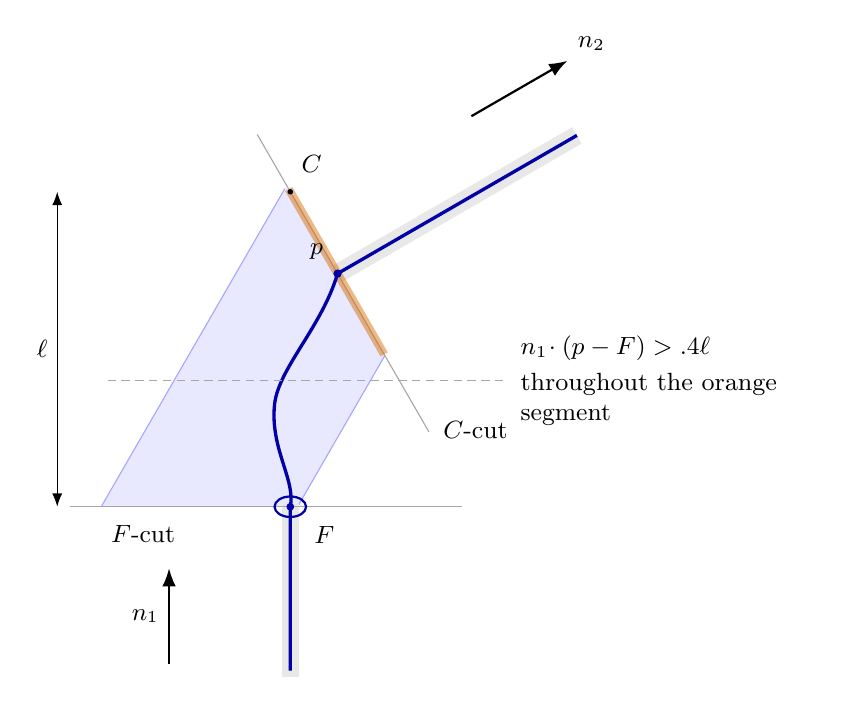
\begin{tikzpicture}[x=2cm,y=2cm,>=Latex,font=\small]
  \fill[blue!9] (-1.200889,0)--(.046188,0)--(.600444,.960000)
       --(-.011547,2.020000)--(-.034641,2.020000)--cycle;
  \draw[blue!35] (-1.200889,0)--(-.034641,2.020000)
       (.046188,0)--(.600444,.960000);
  \fill[gray!18] (-.055,-1.08) rectangle (.055,.018);
  \fill[gray!18] (.270,1.532347)--(1.790,2.409925)
       --(1.850,2.306002)--(.330,1.428424)--cycle;
  \draw[gray!70] (-1.40,0)--(1.09,0);
  \draw[gray!70] (-.21,2.363731)--(.88,.475795);
  \node[anchor=north west] at (-1.20,-.06) {$F$-cut};
  \node[anchor=west] at (.91,.49) {$C$-cut};
  \fill[blue!65!black] (0,0) circle (1.4pt);
  \draw[blue!65!black,thick] (0,0) ellipse[x radius=.10,y radius=.065];
  \draw[orange!85!black,line width=3pt,opacity=.48]
       (-.010,2.017321)--(.596,.967698);
  \node[anchor=north west] at (.09,-.065) {$F$};
  \fill[black] (0,2) circle (1.0pt);
  \node[anchor=south west] at (.01,2.06) {$C$};
  \draw[very thick,blue!65!black]
       (0,-1.04)--(0,0)
       .. controls (.035,.17) and (-.13,.37) .. (-.10,.65)
       .. controls (-.075,.88) and (.20,1.14) .. (.30,1.480385)
       --(1.82,2.357963);
  \fill[blue!65!black] (.30,1.480385) circle (1.5pt);
  \node[anchor=south east] at (.27,1.51) {$p$};
  \draw[densely dashed,gray!70] (-1.16,.8)--(1.37,.8);
  \node[anchor=west,text width=3.8cm] at (1.40,.8)
       {$n_1\!\cdot(p-F)>.4\ell$\vspace{2pt}\\
        throughout the orange segment};
  \draw[<->] (-1.48,0)--node[left] {$\ell$}(-1.48,2);
  \draw[->,thick] (-.77,-1.00)--node[midway,left] {$n_1$}(-.77,-.39);
  \draw[->,thick] (1.15,2.48)--(1.76,2.832184)
       node[above right] {$n_2$};
\end{tikzpicture}
\caption{Two recovery cuts at a $60^\circ$ turn, with
$F=C-\ell n_1$ and $n_1\cdot n_2=1/2$. The shaded short region is
bounded by the side walls and the $C$-cut. Its outgoing ports (orange)
lie more than $.4\ell$ above $F$ in the $n_1$ direction; the next tube
remains above $.3\ell$. Thus the two local port regions stay separated
as the cut lines vary. Tubes and path are schematic.}
\label{fig:08-two-cut-corner}
\end{figure}



Choose the finitely many corner lengths successively, with each much
larger than the accumulated endpoint errors from the preceding stages.
Choose the first length so small that the last is still a small fraction
of every original segment. Then choose all cut ranges and tube widths
smaller still. These are choices of fixed constants: every allowed
cut band contains at least $cH$ lattice levels when $H$ is large.
The endpoint of one stage may move over its actual lattice ports; the
next stage is started at that actual endpoint. Equation
\eqref{eq:08-corner-clearance} and the positive scalar products preserve
all clearances uniformly over these choices.

Each long stage has mass at least $cH^{-1/4}$ by
Lemma~\ref{lem:08-free-tube}; the preceding convex construction gives
that bound for each short corner stage. Adjacent stages occupy opposite
strict half-planes of their joining line. Nonadjacent stage regions are
disjoint, after making the widths sufficiently small. Consequently their
concatenation is self-avoiding and its weights multiply. If there are
$m$ stages and $F(\gamma)$ counts their representations of an output
path, summing the $m-1$ joining levels and all the intermediate ports gives
\begin{equation}\label{eq:08-corridor-first}
 \sum_\gamma \rho^{|\gamma|}F(\gamma)
 \ge cH^{-m/4}H^{m-1}.
\end{equation}
No separate endpoint-position factor occurs: it is already included in
each stage's free-terminal mass.

We next give the second-moment argument, including the upper bounds for
the pieces that remain after two representations are cut. Each joining
port region is visited only by its two adjacent stages. At the first
cut of a corner this region is close to $F$; at the second it is within
$O(\ell)$ of $C$ and has the positive separation
\eqref{eq:08-corner-clearance} from $F$. Hence, in any two
representations, both splits at one joint precede both splits at the
next joint. Otherwise the intervening portion would belong to
nonadjacent stage regions, which are disjoint. At a single joint, the
portion between its two split times stays strictly between the two
parallel joining lines, by the opposite half-plane restrictions in the
two representations. It is therefore a bridge. Equal levels give the
same split and port; the corresponding bridge has weight $B_0=1$.

Delete these $m-1$ short bridge gaps. Exactly $m$ portions remain: one
before the first pair of splits, one between every consecutive pair, and
one after the last. Each starts on its incoming supporting line and
stays strictly on its forward side. It ends on its outgoing supporting
line at normal distance at least $\kappa H$ into that forward half-plane,
where $\kappa>0$ depends only on the fixed geometry. For a long stage this
is the segment length less the two narrow cut bands. For a corner it is
\eqref{eq:08-corner-clearance}, less the cut shifts. These conclusions
hold for a mixed pair of representations: retaining the later incoming
split and the earlier outgoing split only moves the relevant lines
within their already allowed bands.

For completeness, this depth gives an upper mass $CB_{\lfloor\kappa H\rfloor}$
for each remaining portion. Enclose it in the convex intersection of
its endpoint half-planes and distant lattice walls. Its source is on
the incoming wall. Cut this domain by a line parallel to that wall at
depth $\kappa H/2$. Every allowed terminal port is lost in the cut.
Lemma~\ref{lem:08-localization} bounds their total mass by the new-cut
mass, which is at most $CB_{\lfloor\kappa H/2\rfloor}\le CH^{-1/4}$.
This estimate is uniform in the actual starting port. We can thus sum
the portions in their temporal order, dropping mutual avoidance for an
upper bound, without paying for another translation or for a new root.

For each joint the sum over its two levels and their bridge gap is at
most
\[
 CH\sum_{g=0}^{CH}B_g\le CH^{7/4}.
\]
The $m$ macroscopic portions therefore give
\begin{equation}\label{eq:08-corridor-second}
 \sum_\gamma\rho^{|\gamma|}F(\gamma)^2
 \le CH^{-m/4}H^{7(m-1)/4}.
\end{equation}
The finitely many choices of the order of two levels are included in
$C$. Weighted Cauchy--Schwarz, applied to
\eqref{eq:08-corridor-first} and \eqref{eq:08-corridor-second}, yields
\[
 \sum_{F(\gamma)>0}\rho^{|\gamma|}
 \ge cH^{-m/4+2(m-1)-7(m-1)/4}=cH^{-1/4}.
\]
This proves the asserted finite-chain estimate with no exponent loss.

We now fit such a chain to the obstacle. We may decrease $\delta$ below
one and increase $D$ above one. If $v-u\le\delta H/2$, a sufficiently
narrow vertical free tube stays to the right of $x-\delta H$ and has
mass at least $c(1+v-u)^{-1/4}\ge c'H^{-1/4}$; zero and bounded gaps
cost only fixed elementary paths. Otherwise rise a small fixed fraction
of $\delta H$, then take one right-up segment and a fixed number of right-down/right-up pairs, with normals
$(\sqrt3/2,-1/2)$ and $(\sqrt3/2,1/2)$. Choose equal segment lengths
in each pair, much smaller than $\delta H$, and use sufficiently many
pairs that the horizontal coordinate exceeds $x+(D+1)H$. The last
oblique direction is right-up, so it has scalar product $1/2$ with
the final upward direction. Keep this
part in the first $\delta H/2$ bands, and finish by rising vertically
to $y=v$. There is fixed proportional clearance from the obstacle and
from both horizontal walls except at the required endpoints. Adjacent
normals have scalar product $1/2$; the stages are simple and separated
at all nonadjacent segments. The two-cut construction just proved fits
inside this clearance. All lengths and the enclosing box are fixed
multiples of $H$, depending only on $D,\delta$. This proves the lemma.
\end{proof}

\begin{corollary}[A long arch in a shallow strip]\label{lem:08-long-arch}
For every fixed $\sigma>0$ and all sufficiently large fixed $D'$, there
are $c,C>0$ and $h_0$ with the following property for $h\ge h_0$. From any horizontal boundary port $a=(x_A,u)$,
there is arch mass between $ch^{-1/4}$ and $Ch^{-1/4}$ which stays in
\[
 u<y<u+\sigma h,\qquad x>x_A-\sigma h,
\]
except at its two boundary endpoints, and has free terminal port on
$y=u$ with abscissa exceeding $x_A+D'h$. The arches can be confined
to a box of diameter $Ch$.
\end{corollary}
\begin{proof}
Use the same normal-direction chain as in
Lemma~\ref{lem:08-sharp-corridor}: rise first, make equal right-up and
right-down pairs inside a small fraction of the $\sigma h$-high slab,
and end with a downward segment beyond $x_A+(D'+1)h$. Choose the last
oblique direction right-down, so its scalar product with the final
downward direction is $1/2$. All intermediate regions lie strictly
above the starting line, and the final downward tube ends on that line.
They remain right of $x_A-\sigma h$ with fixed proportional clearance.
The finite-chain estimate gives the lower bound. The terminal
displacement forces lateral extent at least $D'h$. For
$D'\ge C_1\sigma$, Lemma~\ref{lem:08-localization} bounds the total
such arch mass in the height-$\lceil\sigma h\rceil$ strip by
$C\sigma h(D'h)^{-5/4}\le C'h^{-1/4}$. Lattice rounding changes only
fixed constants.
\end{proof}

\section{From localized moments to a typical bridge}\label{sec:renewal}

Proposition~\ref{prop:08-localized-length} turns the confined first and
second moments into the following seed estimate: for every fixed
\(\xi>0\),
\[
 \Prob_h^{\rm br}\{|\gamma|\ge h^{4/3-\xi}\}\ge h^{-o(1)}.
\]
This probability may tend to zero. We amplify it to a high-probability
length bound by running independent irreducible-bridge trials, then
pay explicitly for conditioning on a specified terminal height.

The irreducible-bridge construction goes back to Kesten's renewal
identity~\cite{Kesten1963}; see Madras--Slade~\cite{MadrasSlade1993}
and the appendix of Lawler--Schramm--Werner~\cite{LSW2004}.
We derive the normalization and the conditional renewal estimates
needed for the present port convention.

A bridge is \emph{irreducible} if it has positive height and no
once-crossed intermediate level. Cutting at all such levels gives a unique
sequence of irreducible bridges. Conversely any sequence concatenates
freely: the pieces occupy successive disjoint open strips and their port
weights multiply. Let \(I_h\) be the total irreducible mass at height
\(h\ge1\), and set
\[
 I(z)=\sum_{h\ge1}I_hz^h,\qquad B(z)=\sum_{h\ge0}B_hz^h.
\]
Uniqueness gives \(B(z)=(1-I(z))^{-1}\) for \(0\le z<1\).
Since \(B_h\asymp(1+h)^{-1/4}\),
\[
 B(e^{-1/l})\asymp l^{3/4},\qquad
 \sum_{h\ge1}I_h=1,\qquad \sum_{h\ge l}I_h\le Cl^{-3/4}.
\]
For the tail, use
\((1-e^{-1})\sum_{h\ge l}I_h\le1-I(e^{-1/l})\); normalization follows
by letting \(z\uparrow1\).

We may therefore sample independent irreducible bridges, giving each
individual bridge probability equal to its critical weight. Their
concatenation is an infinite self-avoiding walk in the half-plane. Write
\(U_0=0<U_1<U_2<\cdots\) for its renewal heights, and let
\[
 T(l)=\min\{k:U_k>l\},\qquad G_l=\text{the prefix ending at }U_{T(l)}.
\]
The renewal heights tend to infinity because their increments are positive
integers. The event \(\mathcal H_h=\{h=U_k\text{ for some }k\}\) has probability
\(B_h\). Conditional on \(\mathcal H_h\), the prefix ending at height \(h\)
has exactly the critical height-\(h\) bridge law, normalized by \(B_h\).
This follows path by path from the unique irreducible decomposition.
The analogous strip-conditioning identity in the square-lattice vertex
convention appears in \cite[Proposition 2.10]{DyhrEtAl2011}; its final
bond lies above the conditioning height.

\begin{lemma}[Renewal overshoots and a successful trial]
\label{lem:08-renewal-trial}
For \(x\ge2l\ge2\),
\[
 \Prob\{U_{T(l)}>x\}\le C(l/x)^{3/4}.
\]
For every fixed \(\xi>0\), a trial beginning at a renewal and ending at
the first renewal more than \(h\) bands above it has probability at least
\(h^{-o(1)}\) of containing \(h^{4/3-\xi}\) vertices.
\end{lemma}
\begin{proof}
The last renewal before crossing \(l\) is some \(i\le l\), and its next
increment must exceed \(x-i\). Hence
\[
 \Prob\{U_{T(l)}>x\}
 =\sum_{i=0}^{l}B_i\sum_{j>x-i}I_j
 \le Cx^{-3/4}\sum_{i=0}^{l}B_i
 \le C(l/x)^{3/4}.
\]
For the second assertion let \(Z_h\) count renewals
\(m\in[h/2,h]\) whose prefixes have length at least
\(h^{4/3-\xi}\). Applying \eqref{eq:R-32d} with slack \(\xi/2\),
which absorbs the constant factor between \(m\) and \(h\), gives
\(\E Z_h\ge h^{3/4-o(1)}\). The unrestricted number \(N_h\) of
renewals up to \(h\) satisfies
\[
 \E N_h^2
 \le\sum_{m\le h}B_m+
       2\sum_{m<n\le h}B_mB_{n-m}
 \le Ch^{3/2}.
\]
The product in the second sum follows from independence after a renewal.
Thus \(\Prob\{Z_h>0\}\ge(\E Z_h)^2/\E N_h^2\ge h^{-o(1)}\).
Every prefix counted by \(Z_h\) lies in the trial.
\end{proof}

\begin{theorem}[Typical finite-bridge length]
\label{thm:08-bridge-length}
For every \(\varepsilon>0\) there is \(c_\varepsilon>0\) such that a
critical height-\(H\) bridge satisfies
\[
 \Prob_H^{\mathrm{br}}\{H^{4/3-\varepsilon}\le|\gamma|
                         \le H^{4/3+\varepsilon}\}
       \ge1-O_\varepsilon(H^{-c_\varepsilon}).
\]
Its diameter is at least \(d_0H\) and at most \(CH^{1+\varepsilon}\)
with polynomially small exceptional probability.
\end{theorem}
\begin{proof}
Fix small \(\theta,\xi>0\), and put
\[
 h=\lfloor H^{1-\theta}\rfloor,\qquad
 R=\lfloor H^{1-\theta/2}\rfloor,\qquad
 K=\lfloor H^{\theta/16}\rfloor.
\]
Run \(K\) successive trials of Lemma~\ref{lem:08-renewal-trial},
restarting at each completion. Independence of irreducible pieces after
these stopping renewal indices makes the trials independent. If
\(\Delta_j\) is their height advance, then
\[
 \Prob\left\{\sum_{j=1}^K\Delta_j>R\right\}
 \le\sum_{j=1}^K\Prob\{\Delta_j>R/K\}
 \le CK(hK/R)^{3/4}
 \le CH^{-17\theta/64}.
\]
For large \(H\) every trial succeeds with probability at least
\(H^{-\theta/32}\), by its \(h^{-o(1)}\) lower bound. Thus all trials
fail with probability at most \(\exp(-cH^{\theta/32})\). Outside these
two events, a successful trial is contained in \(G_R\). Choose
\(\theta,\xi\) so that
\((1-\theta)(4/3-\xi)>4/3-\varepsilon\). Then
\[
 \Prob\{|G_R|<H^{4/3-\varepsilon}\}
       \le CH^{-17\theta/64}+\exp(-cH^{\theta/32}).
\]

We transfer this estimate to conditioning on \(\mathcal H_H\). Put
\(\tau=T(R)\) and extend \(B_j\) by zero for \(j<0\). For any event
\(E\) determined by the prefix through \(\tau\), renewal independence
gives the exact identity
\[
 \Prob(E\mid \mathcal H_H)
    =\frac{\E[\mathbf1_E B_{H-U_\tau}]}{B_H}.
\]
Here \(R<H\), so a path which overshoots \(H\) at \(\tau\) could not
have hit \(H\) earlier. On \(U_\tau\le H/2\) the density ratio is
bounded by a constant. For all sufficiently large \(H\), we have \(R\le H/4\).
For the remaining conditional probability, let \(i\le R\) be the last
renewal before crossing \(R\), and let \(l\) be the height of the
crossing irreducible. If \(i+l>H/2\), then \(l\ge H/2-R\).
Summing over these possibilities gives the upper bound
\[
 \frac1{B_H}
 \sum_{l\ge H/2-R} I_l
       \sum_{i=0}^{\min(R,H-l)}B_iB_{H-l-i}
 \le C(R/H)^{1/2}.
\]
For completeness, writing
\(C_R(n)=\sum_{i=0}^{\min(R,n)}B_iB_{n-i}\), the full convolution
bound gives \(C_R(n)\le C(n+1)^{1/2}\le CR^{1/2}\) when
\(n\le2R\). When \(n>2R\), use
\(C_R(n)\le CR^{3/4}n^{-1/4}\le CR^{1/2}\).
Multiply this uniform bound by
\(\sum_{l\ge H/2-R}I_l\le CH^{-3/4}\) and
\(B_H^{-1}\le CH^{1/4}\). This proves the displayed estimate.
The prefix \(G_R\) is part of the conditioned height-\(H\) bridge
whenever its endpoint is at most \(H/2\), so the lower-length failure
is \(O(H^{-\theta/4})\). For example, for \(0<\varepsilon<1\),
\(\theta=\varepsilon/8\) and \(\xi=\varepsilon/4\) give the explicit
bound \(O_\varepsilon(H^{-\varepsilon/32})\).

The full strip first-length estimate in
Theorem~\ref{prop:02-length-reduction}, divided by \(B_H\), gives
\(\E_H^{\mathrm{br}}|\gamma|\le H^{4/3+o(1)}\). Markov's inequality proves the
upper bound with polynomially small failure. Finally, dividing the lateral
loss \(CHM^{-5/4}\) of Lemma~\ref{lem:08-localization} by \(B_H\) gives
\(\Prob_H^{\mathrm{br}}\{\text{lateral extent}>M\}\le C(H/M)^{5/4}\).
Take \(M=H^{1+\varepsilon}\). The deterministic height span is \(d_0H\),
which also proves the lower diameter bound.
\end{proof}

\section{Ordered renewal probes}
\label{sec:10-thermal-probes}

Two adjacent pieces of a self-avoiding path cannot pass through each
other. We quantify this elementary obstruction under the independent
renewal law before imposing the eventual height or length of either
piece. The estimate must also allow a single long irreducible bridge to
be inspected from both ends. Those two inspections share the same
critical weight, so their costs cannot be multiplied as independent
probabilities.

Throughout this section, heights count lattice bands, port paths carry
weight $\rho^{|\gamma|}$, and $|\gamma|$ counts visited vertices. Put
$\alpha=3/4$. We use the bridge masses
$B_j\asymp(1+j)^{\alpha-1}$, with $B_0=1$, the localization and kernel
variation estimates of Lemmas~\ref{lem:08-localization}
and~\ref{lem:08-variation}, the free-end tubes of
Lemma~\ref{lem:08-free-tube}, and the corridor construction of
Corollary~\ref{lem:08-long-arch}. A free endpoint is summed over its lattice
ports; once its shape is specified, attaching it to another path makes
its translation unique.

The argument has three parts. First we fix the probability and
unnormalized measures used in every probe. Next a recoverable hairpin
construction bounds masses of pairs with suitably separated renewal
endpoints. Finally we show that, except for a controlled exceptional
part, an ordered probe supplies many such endpoints. This last step
uses its conditional failure bound before conditioning on continued
avoidance.

\subsection{Stopped paths and renewal occurrences}

Write \(\nu(I)=\rho^{|I|}\) for the probability mass of a rooted
irreducible strict port bridge, with the endpoint convention already used
in bridge factorization. Thus \(\sum_I\nu(I)=1\). Let \(\mathbf P\) be
the product law of an infinite sequence of such bridges, with renewal
heights \(U_0=0,U_1,\ldots\). For every real threshold $t\ge0$, let \(\mathcal Q_t\) be the law of its
prefix through the first renewal at or above \(t\). For \(t=0\) this is
the empty prefix. In contrast, define the renewal-occurrence measure
\(\mathcal R\) on finite strings by
\[
 \int G(P)\,d\mathcal R(P)
   =\mathbf E\sum_{k\ge0}G(I_1\cdots I_k).
\]
At fixed height \(j\) this is exactly the unnormalized bridge measure;
its endpoint marginal is \(b_j(x)\), summed with counting measure over
lattice ports \(x\), and its total mass is \(B_j\).
In particular \(\mathcal Q_t\) is a probability measure, whereas
\(\mathcal R\{P:\operatorname{ht}(P)\le t\}\asymp(1+t)^\alpha\).

Whenever a renewal prefix of height \(v\ge t\) is marked, it can be cut
at its first renewal \(U\ge t\). Its exact measure is
\(d\mathcal Q_t(P)\,d\mathcal R(R)\), with the residual-height condition
\(U+\operatorname{ht}(R)=v\). For a sum over \(v\le Ct\), the residual
mass is uniformly at most \(C(1+t)^\alpha\). The empty residual string
is included. This identity, rather than conditioning a bridge to hit a
specified terminal height, is the change of measure used below.

\begin{lemma}[Jump charges and renewal counts]
\label{lem:10-charges}
For an irreducible bridge let \(J\) be its height and \(W\) its maximum
absolute horizontal displacement from its start. For dyadic \(a\ge1\) and real $d\ge0$,
\[
 \mathbf P\{a\le J<2a,\ W\ge da\}
 \le Ca^{-\alpha}\Phi(d),\qquad \Phi(d)=(1+d)^{-5/4}.
\]
Moreover, for $b\ge0$ and \(x\ge1\),
\[
 \mathbf E\sum_{k:U_{k-1}<b}
 \min\{1,(J_k+W_k)/x\}
 \le C(1+b)^\alpha x^{-\alpha}.
\]
For every positive integer $p$, the number of renewals in any height interval of length \(v\ge0\), after a stopping
renewal, has \(p\)-th moment at most
\(C_p(1+v)^{p\alpha}\), uniformly in the stopping history and interval
location.
\end{lemma}

\begin{proof}
Prepend and append bridges with heights in \([a,2a]\) to a marked
irreducible. Their product mass is at least \(ca^{2\alpha}\). Output
heights are \(O(a)\), and a marked irreducible of height at least \(a\)
has bounded multiplicity in such an output. Its lateral excursion forces
comparable output range. The strip lateral estimate bounds output mass
by \(Ca^\alpha\Phi(d)\), proving the first assertion. Summing dyadic
\(a\) and width bins gives
\(\mathbf E\min\{1,(J+W)/x\}\le Cx^{-\alpha}\).
The event \(U_{k-1}<b\) is decided before jump \(k\); multiplying by the
fresh-jump expectation and summing gives the charge estimate, because
\(\sum_{j<b}B_j\le C(1+b)^\alpha\). This includes the last, possibly
overshooting jump. For the moment estimate, order the marked renewals,
restart at each, and sum their nonnegative height increments using
\(\sum_{j\le v}B_j\le C(1+v)^\alpha\). Diagonal repetitions cost only
a constant depending on \(p\). A delayed interval is handled by first
stopping on entrance; overshoot can only shorten its remaining length.
\end{proof}

Launch two independent renewal strings at neighboring ports on one line.
The left and right designations specify their launch order. The test
\(E(h)\), measurable under \(\mathcal Q_h\otimes\mathcal Q_h\), requires
disjointness at depths \(0\le y<h\) and, at every such depth,
\[
 \begin{aligned}
 \max x(\text{left arc at }y)&\le\max x(\text{right arc at }y),\\
 \min x(\text{left arc at }y)&\le\min x(\text{right arc at }y).
 \end{aligned}
\]
It is enough to use depths intersecting the embedded edges. Strict
renewals prevent later visits below their level, so \(E(h)\) implies
all smaller-depth tests. This is an ordered test; disjointness alone of
the two stopped strings is not its definition.

Fix constants \(L_2\ge L>1\), to be selected below. A dyadic height is $2^k$ with $k\in\mathbb Z_{\ge0}$. For dyadic \(r\ge h\),
let \(F(h,r,d)\) be the probability of \(E(h)\) together with a jump
\(I\) of a designated arm satisfying \(r\le J(I)<2r\), \(W(I)\ge dr\),
and born before height \(h/L\). Such a jump is unique: after it the renewal height is at least $h$, so a second jump cannot be born in the specified window. Equivalently,
\begin{equation}
 F(h,r,d)=
 \int_{\operatorname{ht}(P)<h/L}\!d\mathcal R(P)
 \sum_{\substack{r\le J(I)<2r\\W(I)\ge dr}}\nu(I)
 \int \mathbf1_{E(h)}(PI,A)\,d\mathcal Q_h(A).
 \label{eq:10-F-integral}
\end{equation}
The obstacle \(PI\) already contains its stop at \(h\).

For the paired quantity use the same irreducible \(I\) from its two ends,
reversing and reflecting it as needed. Precede it, in these separate
inward orientations, by prefixes \(P_i\) of height \(f_i<h_i/L_2\),
and launch independent workers \(A_i\) at adjacent ports. There is no
avoidance condition between the two sides. Its precise definition is
\begin{equation}
 \begin{split}
 F_{12}(h_1,h_2,r)
 ={}&\sum_{r\le J(I)<2r}\nu(I)
 \int_{f_1<h_1/L_2}\!d\mathcal R(P_1)
 \int_{f_2<h_2/L_2}\!d\mathcal R(P_2)\\[-2mm]
 &\quad\times\prod_{i=1}^2
 \left[\int\mathbf1_{E(h_i)}(P_iI^{(i)},A_i)
                    d\mathcal Q_{h_i}(A_i)\right].
 \end{split}
 \label{eq:10-paired-integral}
\end{equation}
Here \(I^{(1)},I^{(2)}\) are the two normalized orientations of one shape,
not independent jumps. Each side is normalized by its own near launch;
its other ports are determined by concatenation. In particular no
horizontal position is summed in addition to the endpoints already
present in \(d\mathcal R\) and \(\nu\).

Figure~\ref{fig:10-probe-factors} displays the shared and separate
integrations in this definition.

\begin{figure}[ht]
\centering
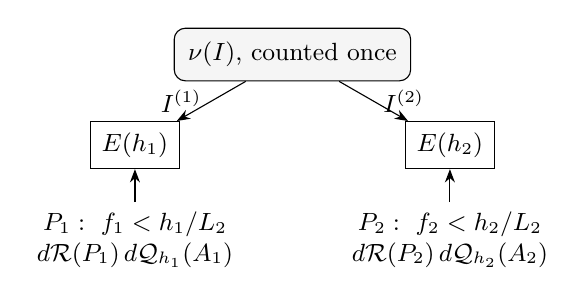
\begin{tikzpicture}[font=\small,>=Stealth,
  mass/.style={draw,rounded corners,inner sep=5pt,fill=black!4},
  test/.style={draw,inner sep=4pt}]
 \node[mass] (giant) at (0,1.7) {$\nu(I)$, counted once};
 \node[test] (e1) at (-2,.55) {$E(h_1)$};
 \node[test] (e2) at (2,.55) {$E(h_2)$};
 \draw[->] (giant)--node[left] {$I^{(1)}$}(e1);
 \draw[->] (giant)--node[right] {$I^{(2)}$}(e2);
 \node[align=center] (p1) at (-2,-.65)
   {$P_1:\ f_1<h_1/L_2$\\$d\mathcal R(P_1)\,d\mathcal Q_{h_1}(A_1)$};
 \node[align=center] (p2) at (2,-.65)
   {$P_2:\ f_2<h_2/L_2$\\$d\mathcal R(P_2)\,d\mathcal Q_{h_2}(A_2)$};
 \draw[->] (p1)--(e1);
 \draw[->] (p2)--(e2);
\end{tikzpicture}
\caption{The integrations defining $F_{12}$. Both tests use one
irreducible bridge. Conditional on that shape, their prefix and worker
integrations separate. Prefix endpoint positions are already summed
by $\mathcal R$; there is no additional translation factor.}
\label{fig:10-probe-factors}
\end{figure}

\begin{theorem}[Ordered probes, with one or two giant ends]
\label{thm:10-ordered-probes}
The constants \(L,L_2,K_1,K_2,K_3\) can be chosen so that, for all integer
\(1\le h,h_1,h_2\le r\), with \(r\) dyadic and \(d\ge0\),
\begin{equation}
 \mathbf P(E(h))\le K_1h^{-\alpha},\qquad
 F(h,r,d)\le K_2r^{-\alpha}\Phi(d),\qquad
 F_{12}(h_1,h_2,r)\le K_3r^{-\alpha}.\label{eq:T-34}
\end{equation}
Either adjacent-port choice and each reflected orientation obey the same
bounds.
\end{theorem}

\subsection{Recovering one or two hairpins}

Fix \(e>0\), \(D<\infty\), and \(0<\sigma<e/10\). A worker bridge
\(A\), launched to the right of an obstacle, is \emph{qualified at scale
\(h\)} if its endpoint height \(u\) lies in \([eh,2h/5]\), the two
shapes are disjoint, \(|x|\le Dh\) on \(A\), and the obstacle satisfies
\[
 x\le Dh\quad(0\le y\le u+\sigma h),\qquad
 x\le x_A-\sigma h\quad(u\le y\le u+\sigma h).
\]
Coordinates are relative to the near launch, and \(x_A\) is the worker
endpoint abscissa. The obstacle may extend arbitrarily far left.
Reflected qualifications are allowed throughout.

Write $\chi_h(O,A)$ for the indicator that the worker bridge $A$
is qualified against the obstacle $O$, with the prescribed neighboring
launches. The three unnormalized masses used below are
\begin{align*}
 Y(h)&=\iint \chi_h(O,A)
 \mathbf1_{\{\operatorname{ht}(A)+2\sigma h\le
                    \operatorname{ht}(O)\le h\}}
 \,d\mathcal R(O)\,d\mathcal R(A),\\
 X_d(h,r)&=\sum_{\substack{r\le J(I)<2r\\W(I)\ge dr}}\nu(I)
 \int_{\operatorname{ht}(P)\le h/8}d\mathcal R(P)
 \int\chi_h(PI,A)\,d\mathcal R(A),\\
 X_{12}(h_1,h_2,r)&=
 \sum_{r\le J(I)<2r}\nu(I)
 \prod_{i=1}^2\left[
 \int_{\operatorname{ht}(P_i)\le h_i/8}d\mathcal R(P_i)
 \int\chi_{h_i}(P_i I^{(i)},A_i)\,d\mathcal R(A_i)
 \right].
\end{align*}
The last line uses the two inward orientations of one irreducible,
exactly as in \eqref{eq:10-paired-integral}. Its factor $\nu(I)$
occurs once. Worker endpoints are summed by $\mathcal R$; these
quantities are masses of endpoint occurrences, not probabilities of
stopped paths. There is no extra horizontal-translation sum.

\begin{lemma}[Hairpin mass bounds]
\label{lem:10-hairpins}
For fixed qualification parameters and all sufficiently large scales,
with \(r\) dyadic, \(1\le h,h_1,h_2\le r\), and \(d\ge0\),
\[
 Y(h)\le Ch^\alpha,\qquad
 X_d(h,r)\le Ch^\alpha r^{-\alpha}\Phi(d),\qquad
 X_{12}(h_1,h_2,r)\le Ch_1^\alpha h_2^\alpha r^{-\alpha}.
\]
Bounded scales can be included by changing constants.
\end{lemma}

\begin{proof}
\emph{Constructing the hairpin.}
Apply Corollary~\ref{lem:08-long-arch} at the worker endpoint. It
supplies an arch contained in the next $\sigma h$ bands, to the right
of $x_A-\sigma h$, whose far endpoint lies beyond $D'h$, for any
sufficiently large fixed $D'$. To pass from the relative displacement
in that lemma to this absolute bound, increase its fixed displacement
constant by $D$, using $|x_A|\le Dh$. Its total critical mass is between
$c h^{-1/4}$ and $C h^{-1/4}$. The lower bound has no exponent loss;
the fixed-endpoint tube bound would not suffice here. The corridor
lemma also establishes the endpoint half-plane bounds needed when
this arch is cut in the second-moment calculation below.

Choose \(z\in[eh/5,eh/3]\). From the far end of the long arch descend by
a narrow bridge to level \(z\), with mass at least \(ch^{-1/4}\).
Continue downward by a bridge of free height in \([2r,4r]\); use \(r=h\)
for \(Y\). Require its portion through depth \(z+1\) from its starting
port to stay within horizontal distance \(D''h\) of that port. This
restriction retains mass at least \(cr^\alpha\). Indeed its failure
probability in the renewal law is small for large \(D''\), by
Lemma~\ref{lem:10-charges}. If \(N\) counts renewals in the desired
terminal interval, then \(\mathbf EN\ge cr^\alpha\) and
\(\mathbf EN^2\le Cr^{2\alpha}\); consequently
\(\mathbf E[N\mathbf1_{\rm failure}]\le
 C r^\alpha\mathbf P(\mathrm{failure})^{1/2}\).
Take \(D''\) large and then \(D'\) much larger.

Join the two near launches by a fixed short arch in the one band on the
opposite side. The resulting path rises from its new lower end, goes
round the long arch, descends along the worker to this short turn, then
rises along the obstacle. Append an upper continuation with height in
\([2r,4r]\). For \(X_{12}\) also make the reflected hairpin at the other
end. Qualification gives all lateral clearances. The two near-end
structures protrude by at most \((2/5+\sigma)h_i\); since \(h_i\le r\)
and the giant has height at least \(r\), they are separated in height.
These operations produce strict bridges at a fixed translated root.
Local connections change weights by fixed factors.
Figure~\ref{fig:10-hairpin-geometry} shows the one-giant construction;
there \(\tau\) is the absolute height of the near launch.
\begin{figure}[htbp]
\centering
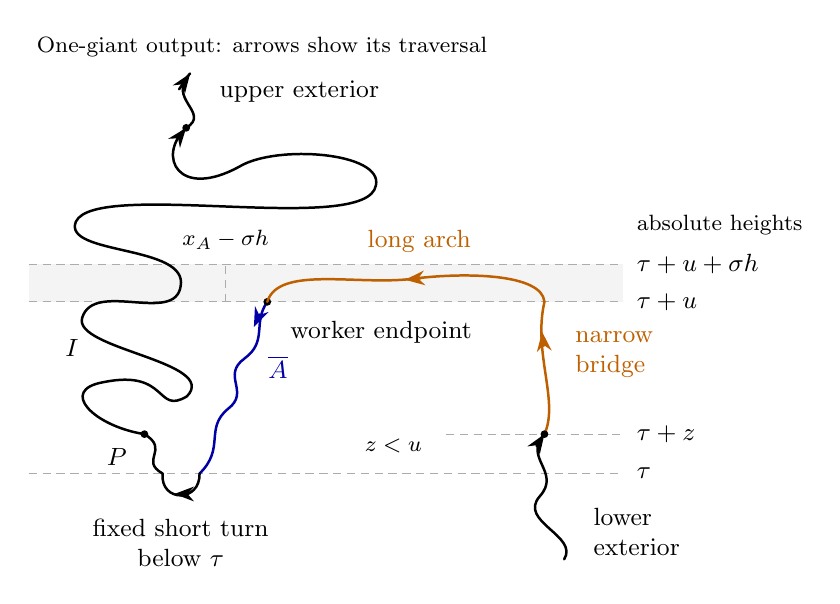
\begin{tikzpicture}[x=1cm,y=1cm,font=\small,>=Stealth,
  pathline/.style={line width=.9pt,line cap=round,line join=round},
  guide/.style={gray!65,densely dashed,line width=.4pt}]
  \fill[gray!9] (.65,3.40) rectangle (8.20,3.88);
  \draw[guide] (.65,3.40)--(8.20,3.40);
  \draw[guide] (.65,3.88)--(8.20,3.88);
  \draw[guide] (3.15,3.40)--(3.15,3.88);
  \node[anchor=south,font=\footnotesize] at (3.15,3.94) {$x_A-\sigma h$};
  \draw[guide] (.65,1.22)--(8.20,1.22);
  \draw[guide] (5.95,1.72)--(8.20,1.72);
  \node[anchor=west] at (8.25,1.22) {$\tau$};
  \node[anchor=west] at (8.25,1.72) {$\tau+z$};
  \node[anchor=west] at (8.25,3.40) {$\tau+u$};
  \node[anchor=west] at (8.25,3.88) {$\tau+u+\sigma h$};
  \node[anchor=west,font=\footnotesize] at (8.25,4.38) {absolute heights};
  \draw[pathline] (2.35,1.22) .. controls (2.05,1.39) and (2.45,1.52) .. (2.12,1.72);
  \draw[pathline] (2.12,1.72)
    .. controls (1.48,1.82) and (1.02,2.28) .. (1.60,2.38)
    .. controls (2.43,2.55) and (2.26,1.96) .. (2.66,2.20)
    .. controls (3.08,2.64) and (1.20,2.80) .. (1.33,3.20)
    .. controls (1.48,3.68) and (2.51,3.11) .. (2.58,3.60)
    .. controls (2.68,4.13) and (1.07,3.99) .. (1.25,4.42)
    .. controls (1.51,4.96) and (4.95,4.23) .. (5.06,4.88)
    .. controls (5.15,5.30) and (3.80,5.40) .. (3.33,5.12)
    .. controls (2.55,4.69) and (2.27,5.25) .. (2.65,5.61);
  \draw[pathline] (2.65,5.61) .. controls (2.97,5.80) and (2.39,5.98) .. (2.70,6.30);
  \draw[->,pathline] (2.58,5.52)--(2.65,5.61);
  \draw[->,pathline] (2.56,6.10)--(2.70,6.30);
  \node[anchor=east] at (2.02,1.43) {$P$};
  \node[fill=white,inner sep=2pt] at (1.20,2.82) {$I$};
  \fill (2.12,1.72) circle (1.4pt);
  \fill (2.65,5.61) circle (1.4pt);
  \node[anchor=west] at (2.95,6.07) {upper exterior};
  \draw[pathline,blue!65!black] (2.82,1.22)
    .. controls (3.15,1.54) and (2.88,1.79) .. (3.18,2.04)
    .. controls (3.47,2.26) and (3.09,2.46) .. (3.39,2.68)
    .. controls (3.69,2.90) and (3.49,3.13) .. (3.68,3.40);
  \draw[->,pathline,blue!65!black] (3.58,3.24)--(3.51,3.08);
  \node[anchor=west,text=blue!65!black] at (3.57,2.57) {$\overline A$};
  \fill (3.68,3.40) circle (1.4pt);
  \node[anchor=north west] at (3.85,3.28) {worker endpoint};
  \draw[pathline] (2.82,1.22) .. controls (2.83,.85) and (2.32,.85) .. (2.35,1.22);
  \draw[->,pathline] (2.64,.96)--(2.50,.96);
  \node[anchor=north,align=center] at (2.58,.77) {fixed short turn\\below $\tau$};
  \draw[pathline,orange!75!black] (7.20,1.72)
    .. controls (7.39,2.14) and (7.05,2.75) .. (7.20,3.40);
  \draw[pathline,orange!75!black] (7.20,3.40)
    .. controls (7.17,3.76) and (6.19,3.78) .. (5.50,3.69)
    .. controls (4.81,3.61) and (3.82,3.86) .. (3.68,3.40);
  \draw[->,pathline,orange!75!black] (5.63,3.70)--(5.43,3.68);
  \draw[->,pathline,orange!75!black] (7.19,2.84)--(7.17,3.02);
  \node[anchor=south,text=orange!75!black] at (5.61,3.91) {long arch};
  \node[anchor=west,align=left,text=orange!75!black] at (7.47,2.73) {narrow\\bridge};
  \draw[pathline] (7.45,.13)
    .. controls (7.64,.43) and (6.86,.61) .. (7.14,.93)
    .. controls (7.42,1.24) and (6.92,1.42) .. (7.20,1.72);
  \draw[->,pathline] (7.10,1.57)--(7.20,1.72);
  \fill (7.20,1.72) circle (1.4pt);
  \node[anchor=west,align=left] at (7.70,.48) {lower\\exterior};
  \node[font=\footnotesize] at (5.28,1.57) {$z<u$};
  \node[anchor=west,font=\footnotesize] at (.63,6.64)
    {One-giant output: arrows show its traversal};
\end{tikzpicture}
\caption{The one-giant hairpin, schematically. From its new lower end the
output follows the right exterior to height $\tau+z$, the narrow bridge
and long arch to the worker endpoint at $\tau+u$, the reversed worker,
the fixed short turn, the prefix $P$, the giant $I$, and the upper
exterior. Here $z\in[eh/5,eh/3]$ and $u\in[eh,2h/5]$ are relative
heights; $\tau$ is the absolute near-launch level. In the shaded slab
the obstacle is to the left of $x_A-\sigma h$ and the long arch is to
its right. The curves are not to scale and indicate joining order and
clearance, not lattice edges or monotonicity. In particular $I$ has no width bound, and the
drawn prefix endpoint has no required height order relative to $u$.}
\label{fig:10-hairpin-geometry}
\end{figure}


\smallskip\noindent\emph{Representation mass and nearby turn lines.}
For the one-giant construction, let $m(\Gamma)$ count the possible
input tuples and joining choices that produce the rooted output bridge
$\Gamma$. Define
\[
 Z_1=\sum_\Gamma\rho^{|\Gamma|}m(\Gamma),\qquad
 V_1=\sum_{m(\Gamma)>0}\rho^{|\Gamma|},\qquad
 M_2=\sum_\Gamma\rho^{|\Gamma|}m(\Gamma)^2.
\]
The weight of an input tuple is comparable to the output weight,
because its pieces partition $\Gamma$ apart from the bounded local
port changes. Thus $Z_1$ is comparable to the summed construction
weight. Weighted Cauchy--Schwarz gives $Z_1^2\le V_1M_2$.
For $X_d=X_d(h,r)$, the preceding construction and the strip lateral
estimate therefore give
\[
 Z_1\ge cX_d r^{2\alpha}h^{1/2},\qquad
 V_1\le Cr^\alpha\Phi(d).
\]
The factor \(h^{1/2}\) is the product of the \(\asymp h\) choices of
\(z\) and the two \(h^{-1/4}\) connector masses. The marked giant's
width forces comparable output range, giving \(\Phi(d)\).

We estimate the second moment by pairs of representations of the same
output. First bin their turn lines \(\tau\), in absolute output coordinates,
into intervals of width \(r/50\). There are only boundedly many such
bins, because output heights are \(O(r)\). Cauchy--Schwarz permits us to
sum same-bin second moments at bounded cost. For turn-line difference
at most \(Nh\), the contribution is
\begin{equation}
 C_Nr^{2\alpha}X_d(h,r)h^{1/2}h^{5/4}.\label{eq:T-35}
\end{equation}
Here is the full cost allocation. Subdivide into intervals of width
\(ceh\), with a sufficiently small fixed \(c\). For nearby cells,
\(ab\le(a^2+b^2)/2\) reduces pair counting to same-cell pairs with a
factor depending on \(N,e\), but no factor for the absolute cell index.
A line strictly between all \(\tau+z\) and all \(\tau+u\) in the cell has the
following property: after its first visit, the lowest point of the path
is the short turn. Before the descending worker reaches that turn, the
initial rising branch stays above \(\tau+z\); afterwards everything other
than the fixed short arch stays above the turn line. Thus the short
turn, its line, and its two bounding visits coincide in the two
representations. The upward branch determines the giant mark up to
bounded choices, since its prefix is at most \(h/8\). Retain the marked
input associated to the smaller worker height \(u\).

Between the two worker heights there are two bridges, one on either
side of the long arch. Their jointly summed cost is
\(\sum_{j\le Ch}B_j^2\le Ch^{1/2}\). The higher long arch costs
\(Ch^{-1/4}\). The far rising bridge from the higher \(z\) to the smaller
\(u\) has height comparable to \(h\), hence costs \(Ch^{-1/4}\).
The pair of \(z\)-levels and their gap cost
\(Ch\sum_{j\le Ch}B_j\le Ch^{1+\alpha}\). Multiplying these four costs
gives \(Ch^{1/2+5/4}\), as in \eqref{eq:T-35}. The two exterior
continuations supply \(r^{2\alpha}\). Ties use \(B_0=1\).
Every cut is determined by its level: each selected \(u\)-level is
crossed twice on the pre-turn part, while the \(z\)-cuts are first
visits before these crossings. A rooted tuple of these relative shapes
has one translation to the prescribed joining port, also when attached
by its far endpoint. Thus no horizontal multiplicity is omitted.

\smallskip\noindent\emph{Distant turn lines.}
For distant turn lines in the same coarse bin, write
\(\Delta=\tau_2-\tau_1>Nh\), and let \(p_i=\tau_i+f_i\) be their giant junctions.
Everything before \(p_1\) has height at most
\(\tau_1+(2/5+\sigma)h<\tau_2+z_2\), since \(\Delta>Nh\).
Thus the first visit to \(\tau_2+z_2\) occurs after \(p_1\).
Moreover, \(\Delta<r/50\) and \(z_2=O(h)\), with \(h<\Delta/N\),
put this cut below the terminal level of the first giant. The portion
from \(p_1\) to this cut is therefore contained in that giant. It is
strict above its lower level by the giant's lower wall, and strict
below its upper level by the first-visit property. After the cut the
second representation never falls below \(\tau_2-O(1)\). If this subbridge had a
single-crossing level below \(\tau_2-O(1)\), it would also be a seam of the
first giant. Its first irreducible \(I'\) consequently has height
\[
 J(I')\in[\Delta-f_1-O(1),\Delta-f_1+O(h)],
\]
and the rest is a bridge of free height \(O(h)\). Replacing the first
giant by \(I'\) preserves the earlier qualification, which concerns
only its near range. Retain this reduced first construction and then
the second construction with its original giant. The very first and
last exterior continuations are retained as well. The removed endpoint
of the first giant is recoverable as its first ensuing renewal in the
upward continuation; it has no unbounded marking multiplicity.

The second construction costs \(h^{1/2}X_d(h,r)\); the reduced first
one at dyad \(a\) costs \(h^{1/2}X_0(h,a)\); the intervening bridge costs
\(h^\alpha\). Hence the distant contribution is at most
\[
 Cr^{2\alpha}h^{1/2}X_d(h,r)\,
 h^{\alpha+1/2}\sum_{Nh/C\le a<r}X_0(h,a).
\]
Relative offsets of the two turn lines are already determined by the
reduced shapes. For \(d=0\), induct on the dyadic \(r\) with the bound
\(X_0(h,a)\le Kh^\alpha a^{-\alpha}\). After division by
\(r^{2\alpha}h^{1/2}X_0(h,r)h^{5/4}\), the distant contribution is at
most \(CKN^{-\alpha}\). Cauchy--Schwarz, \(Z_1^2\le V_1\) times the
second moment, therefore gives
\[
 X_0(h,r)\le h^\alpha r^{-\alpha}(C_N+CKN^{-\alpha}).
\]
Choose \(N\) first to make the coefficient of \(K\) smaller than one
half, then \(K\) to absorb \(C_N\) and the bounded initial scales. For
\(d>0\) use this proved \(X_0\) bound in the distant sum and retain the
factor \(\Phi(d)\) in \(V_1\). This proves the one-giant bound.

For \(Y\), only nearby bins are needed, with \(r=h\). The obstacle's
terminal cut \(v\) is now movable on the common upward branch. Retain
the smaller worker height and smaller obstacle height, even if they
come from different representations. Shortening preserves
qualification and \(v-u\ge2\sigma h\). The larger \(v\) costs one
additional summed bridge gap, at most \(Ch^\alpha\). The same
Cauchy--Schwarz calculation gives \(Y\le Ch^\alpha\).

\smallskip\noindent\emph{Two ends of a shared giant.}
It remains to bound both ends of one giant simultaneously. Use the
analogous representation count for the paired construction. Its first
moment is at least
\(cX_{12}r^{2\alpha}\prod_i h_i^{1/2}\), and output mass is at most
\(Cr^\alpha\). Bin both turn lines into intervals of width \(r/50\).
On side \(i\), color the fine cells of width \(ceh_i\) periodically with
a sufficiently large fixed number of colors. Matching colors mean either
the same cell or separation exceeding \(100h_i\). Splitting into these
finitely many classes and applying Cauchy--Schwarz lets us use only
matching-color pairs.

Call a same-cell side local. The preceding recovery of the short turn
also recovers its giant junction: all seams within the first \(h_i/8\)
bands are unaffected by the other-end hairpin, which lies far beyond
that range. Distinct junctions would put an internal seam in one of the
two giants. On a distant side the outer junction precedes the inner one
in the inward orientation, and the preceding \(I'\)-replacement applies.

We describe the retained subpaths before counting them. Write
\(a_j,b_j\) for the lower and upper giant junctions of representation
\(j\), and write \(\prec\) for order along the oriented output path.
At the lower end denote the two junctions by
\(a_{\rm out}\preceq a_{\rm in}\), and at the upper end by
\(b_{\rm in}\preceq b_{\rm out}\); equality means that side is local.
The subpath between \(a_{\rm in}\) and \(b_{\rm in}\) will be the
central giant. When both sides are distant, the two possible orders,
after interchanging representation names or reflecting, are
\[
 a_1\prec a_2\prec b_1\prec b_2
 \quad\hbox{and}\quad
 a_1\prec a_2\prec b_2\prec b_1.
\]
Thus the central subpath is \([a_2,b_1]\) in the crossed case and
\([a_2,b_2]\) in the nested case. Figure~\ref{fig:10-paired-path-order}
shows these path orders; it does not depict the spatial positions of
the junctions.
\begin{figure}[htbp]
\centering
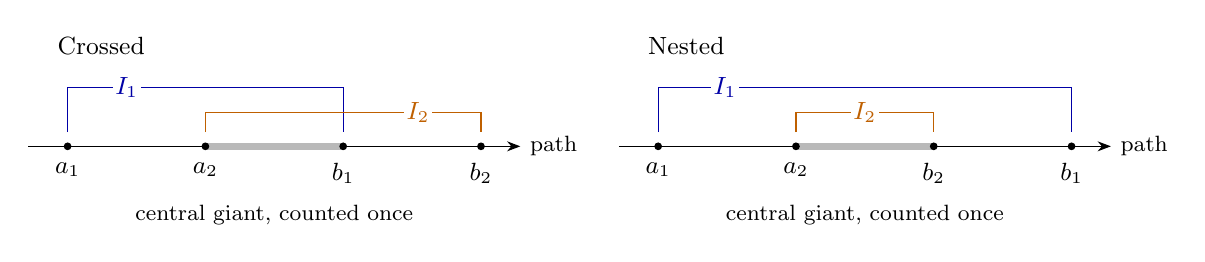
\begin{tikzpicture}[x=1cm,y=1cm,font=\small,>=Stealth]
\foreach \offset/\name/\third/\fourth in {0/Crossed/1/2,7.5/Nested/2/1}{
 \begin{scope}[xshift=\offset cm]
  \node[anchor=west] at (0,1.28) {\name};
  \draw[->] (-.25,0)--(6.0,0) node[anchor=west,font=\footnotesize] {path};
  \draw[line width=2.3pt,gray!55] (2,0)--(3.75,0);
  \foreach \x/\lab in {.25/a_1,2/a_2,3.75/b_{\third},5.5/b_{\fourth}}{
   \fill (\x,0) circle (1.4pt);
   \node[anchor=north] at (\x,-.09) {$\lab$};
  }
  \node[anchor=north,font=\footnotesize] at (2.875,-.62) {central giant, counted once};
 \end{scope}
}
\draw[blue!65!black] (.25,.18)--(.25,.75)--(3.75,.75)--(3.75,.18);
\node[fill=white,inner sep=1pt,text=blue!65!black] at (1.0,.75) {$I_1$};
\draw[orange!75!black] (2,.18)--(2,.43)--(5.5,.43)--(5.5,.18);
\node[fill=white,inner sep=1pt,text=orange!75!black] at (4.7,.43) {$I_2$};
\draw[blue!65!black] (7.75,.18)--(7.75,.75)--(13,.75)--(13,.18);
\node[fill=white,inner sep=1pt,text=blue!65!black] at (8.6,.75) {$I_1$};
\draw[orange!75!black] (9.5,.18)--(9.5,.43)--(11.25,.43)--(11.25,.18);
\node[fill=white,inner sep=1pt,text=orange!75!black] at (10.375,.43) {$I_2$};
\end{tikzpicture}
\caption{Two representations of the same output when both sides are
distant, shown in path order, not in spatial coordinates. In the crossed case
$a_1\prec a_2\prec b_1\prec b_2$, the central giant is $[a_2,b_1]$;
in the nested case $a_1\prec a_2\prec b_2\prec b_1$, it is
$[a_2,b_2]$. The brackets identify the original giants $I_j=[a_j,b_j]$
as recovered subpaths. The two outside junctions are retained by the
reduced inputs. Neither the bracket crossings nor their vertical
positions represent intersections or heights of the walk.}
\label{fig:10-paired-path-order}
\end{figure}


The central subpath is indeed an irreducible bridge of scale \(r\) or
\(r/2\). When both its junctions come from one representation, it is
that representation's giant. In the crossed case it is contained in
both giants: the giant starting at \(a_2\) keeps it strictly above
\(a_2\), and the giant ending at \(b_1\) keeps it strictly below
\(b_1\). Divide its height range into lower and upper halves.
A seam in the lower half would extend to a seam of the
giant \([a_2,b_2]\): between \(b_1\) and \(b_2\), the upper
hairpin can descend below \(b_1\) by at most
\((2/5+\sigma)h_{\rm up}+O(1)\), where \(h_{\rm up}\) is the
upper-side test scale. A seam in its upper half is
excluded by the reflected argument using \([a_1,b_1]\). Each turn-line
difference is less than \(r/50\), and a distant difference exceeds
\(100h_i\), so the near-end excursions cannot invalidate either
extension. The central height can fall below \(r\) only in this
two-distant case, where necessarily \(h_i\le r/2\). On a distant
side retain the inner representation's worker and prefix; on a local
side retain the smaller worker height. They qualify against the central
giant by containment, and so give a central paired input.

\smallskip\noindent\emph{Recovering the paired representations.}
In the crossed case, the lower reduced construction retains the first
representation's worker and prefix, followed by its first irreducible \(I'_-\); thus
\(a_1\) is still the prefix--irreducible junction of that counted
input. On the upper side, read inward from the upper end, the reduced
construction retains the second representation's worker and prefix,
followed by its first irreducible \(I'_+\); its prefix--irreducible
junction is \(b_2\). The remaining endpoints \(a_2,b_1\) are the two
endpoints of the central giant. These are existing input junctions,
rather than additional marks placed on an unmarked bridge.

Here is the order in which the lower pieces are joined. For
\(j=1,2\), write \(A_j,P_j,S_j\) for the lower worker, obstacle
prefix, and fixed short turn, respectively. Let \(K_j\) be the
connector from the cut at \(\tau_j+z_j\), through the narrow
bridge and long arch, to the worker endpoint, retaining their counted
joining ports and local connection data; here
\(\tau_j\) denotes the turn-line height. Let \(R_-\) be the
bridge remainder after \(I'_-\), and let \(E_-\) be the first
exterior continuation. With a bar denoting path reversal, the lower
part of the common output is assembled in the order
\[
 E_-\,K_1\,\overline{A_1}\,S_1\,P_1\,I'_-\,R_-\,
 K_2\,\overline{A_2}\,S_2\,P_2,
\]
and then the central giant is attached. The upper part is assembled
by the reflected reverse procedure, with representation 2 outer and
representation 1 inner. In the forward cutting operation,
\(I'_-\) ends at the first positive renewal of the strict subbridge
from \(a_1\) to the second connector's first-visit cut; \(R_-\)
is the rest of that subbridge. The upper cut uses the same rule in
the reversed orientation. Consequently the reduced-irreducible cuts
require no further renewal index. The connector cuts themselves are
the first-visit and ordered worker cuts already specified above.

Each item in this list is a rooted relative shape: part of the central
or a reduced outer input, a connector, a bridge remainder, or an
exterior continuation. Once one joining port is placed, the next shape
has a unique translation to it, including when the shape is attached
by its terminal port. Its height and horizontal displacement are then
fixed. Starting at the prescribed output root therefore places every
piece, and in particular all four retained junctions, without a
separate sum over turn-line differences or horizontal offsets.
The second lower exterior continuation is the assembled prefix
\(E_-K_1\overline{A_1}S_1P_1I'_-R_-\) ending at the exterior
port of \(K_2\);
the remaining upper exterior is the corresponding recovered suffix.
Thus each original exterior is recovered by cutting at its retained
connector port. Finally, extract the ordered subpaths \([a_1,b_1]\) and
\([a_2,b_2]\), and assign the retained workers, prefixes and
connectors to their recorded representation. This recovers both
original constructions. Interchanging the representation names,
choosing the reflected orientation, and the bounded local connection
choices require only finitely many records.

For the nested two-distant case, the order is
\(a_1\prec a_2\prec b_2\prec b_1\). The central paired input is
bounded by \(a_2,b_2\), both from representation 2, and the two
reduced inputs retain \(a_1,b_1\), both from representation 1.
A finite matching record assigns the four retained boundaries
\(a_{\rm out},a_{\rm in},b_{\rm in},b_{\rm out}\)
to the two representations; the same ordered assembly and exterior-port cuts recover the nested
case. On a local side the two junctions coincide as proved above.
The tuple pieces partition the common output, apart from bounded
port modifications. Their product critical weight is therefore
comparable to the single critical weight of that output in the
second moment. In particular the central giant is charged once;
the two original giants are recovered subpaths of the assembled
output and do not contribute additional weight factors.

The reconstruction has bounded ambiguity, uniformly in all scales.
We can therefore integrate these pieces. Each exterior continuation
costs \(Cr^\alpha\). A local side has the four gap and arch costs
already computed, namely \(Ch_i^{1/2+5/4}\). On a distant side the
inner connector costs \(Ch_i^{1/2}\), the reduced outer construction
costs \(Ch_i^{1/2}X_0(h_i,a)\), and the bridge remainder costs
\(Ch_i^\alpha\). The proved one-sided estimate gives
\[
 h_i^{1/2}h_i^{1/2}h_i^\alpha
       \sum_{a\ge c h_i}X_0(h_i,a)
 \le Ch_i^{1+\alpha}=Ch_i^{1/2+5/4}.
\]
The central paired input has scale \(r\) or \(r/2\), and its giant
weight is charged once. Combining these costs with the first moment
and output mass yields
\[
 \begin{split}
 &\left(cX_{12}(h_1,h_2,r)r^{2\alpha}\prod_i h_i^{1/2}\right)^2\\
 &\qquad\le Cr^{3\alpha}\prod_i h_i^{1/2+5/4}
  \{X_{12}(h_1,h_2,r)+X_{12}(h_1,h_2,r/2)\},
 \end{split}
\]
omitting an out-of-domain last term. Writing
\(V_r=X_{12}(h_1,h_2,r)/(h_1^\alpha h_2^\alpha r^{-\alpha})\),
this becomes
\(V_r^2\le C(V_r+2^\alpha V_{r/2})\). A sufficiently large constant
majorant closes the dyadic induction, proving the paired bound.
\end{proof}

\subsection{Finding separated renewal endpoints}

\begin{lemma}[Usable renewals after a regular history]
\label{lem:10-usable-renewals}
Stop a worker at its first renewal at or above \(s\), where \(s/h\) is
a sufficiently small fixed constant. Call this history regular when
the sum of \(J+W\), including its last jump, is less than \(h/16\).
For every \(\delta>0\) one can choose fixed qualification parameters so
that, for all sufficiently large \(h\) depending on these choices,
conditionally on any such history and any fixed opposite path,
with failure probability at most \(\delta\), continued \(E(h)\) implies
at least \(c h^\alpha\) qualified worker renewals in \([eh,2h/5]\).
For two workers with regular histories, outside total conditional failure
probability at most \(2\delta\), continued \(E(h)\) supplies at least
\(ch^{2\alpha}\) separated renewal pairs. In each pair the lower renewal
is a qualified worker against the opposite prefix ending at the higher
renewal, whose height exceeds it by at least \(2\sigma h\).
The failure probabilities are taken before conditioning on continued
\(E(h)\).
\end{lemma}

\begin{proof}
Write \((t,x_0)\) for the worker stop. A regular history has
\(t<h/16\) and horizontal range less than \(h/16\). For
\(m=\lceil3c'h^\alpha\rceil\), the probability that the next \(m\)
jumps advance more than \(h/4\) is \(O(c')\): bound jumps larger than
\(h/4\) by a union bound and the remaining sum by its truncated mean.
Choose \(c'\) small. There are then at least \(2c'h^\alpha\) future
renewals before \(t+h/4<2h/5\), except with arbitrarily small
probability. Renewals within \(eh\) of the stop have expected count
\(O((1+eh)^\alpha)\), so remove them by taking \(e\) small.

No short bin contains a substantial fraction of these renewals with
high probability. Indeed partition the candidate interval into
\(O(\theta^{-1})\) bins of length \(\theta h\). By
Lemma~\ref{lem:10-charges}, for any fixed \(p>1/\alpha\), the probability
that some bin contains at least \(\varepsilon h^\alpha\) renewals is at
most \(C_{p,\varepsilon}\theta^{p\alpha-1}\), once \(\theta h\) is
large. Use neighboring bins as well to control every interval of length
\(2\theta h\). The charge bound also makes the entire worker's lateral
range through its test stop at \(h\) at most \(Dh\), with failure
probability \(O(D^{-\alpha})\).

Freeze the opposite path. For a right worker let \(R(u)\) be the
rightmost opposite abscissa in \([u,u+\sigma h]\). From \((t,x_0)\)
the renewal-occurrence density at \((u,x)\) is exactly
\(b_{u-t}(x-x_0)\). It is not divided by \(B_{u-t}\), since we count
renewal occurrences. Thus the expected number of renewals, at distance
at least \(eh\) above the stop, with \(|x-R(u)|\le2e'h\), is at most
\begin{align*}
 C(e'h+1)\sum_{j\ge eh}\|b_j\|_\infty
 &\le C(e'h+1)\sum_{j\ge eh}(B_j-B_{j+1})\\
 &\le C_e(e'+h^{-1})h^\alpha.
\end{align*}
The middle inequality follows from Lemma~\ref{lem:08-variation}: a summable nonnegative kernel tends to zero at infinity, so its supremum is at most its total variation. The sum of the resulting differences telescopes. No height-by-height derivative bound on $B_j$ is needed.
At each renewal \(u\), restart and discard it if the path through its
first renewal strictly above \(u+\sigma h\) moves more than \(e'h\)
laterally. Its conditional probability is at most
\(C((1+\sigma h)/(e'h))^\alpha\); multiplying by the expected candidate
count bounds the expected number discarded by this quantity times
\(Ch^\alpha\).

On continued order, every opposite point in this slab lies to the left
of the worker's rightmost point at that level. For a retained candidate
that point is at most \(x+e'h\), because strict renewals exclude earlier
and later pieces from the slab. Hence \(R(u)\le x+e'h\). Since
\(|x-R(u)|>2e'h\), necessarily \(R(u)<x-2e'h\). Choose
\(\sigma<e'\). This is the required clearance; the obstacle's global
one-sided bound below \(u+\sigma h\) follows from order and the worker's
bounded range. Reflection gives the other orientation.

Choose the constants successively: the desired failure tolerance,
\(c'\), then \(e,\theta\), then \(D\) large and \(e'\) small, and finally
\(\sigma\) small relative to \(e',e,\theta\). The expectation bounds and
Markov's inequality leave \(ch^\alpha\) candidates. For two workers,
apply this uniform estimate first with the opposite future frozen and
then with roles reversed, integrating by Tonelli. A union bound suffices;
independence of the two good events is unnecessary. Bin nonconcentration
ensures that only a small fraction of all cross-pairs have heights
within \(2\sigma h\). The remaining pairs have the claimed lower/higher
qualification.
\end{proof}

The preceding lemma converts a regular stopped history into many
qualified endpoints. To use it without biasing the fresh jumps, we
will retain a smaller test that is measurable at the stopping time,
then bound failures under the original conditional law. Before doing
so, we record the dyadic estimates that control irregular histories.

\subsection{The ordered-probe induction}

We record the elementary dyadic sums that close the proof. Let \(a\)
range over positive dyadic heights and let \(l\) range over
\(0,2,4,8,\ldots\); the bin \(l=0\) means \(W/a<2\). Put
\[
 T_h(a,l)=\min\{1,(1+l)a/h\}.
\]
Since \(\sum_l(1+l)\Phi(l)<\infty\) on these dyads,
\begin{align}
 \sum_{a,l}a^{-\alpha}\Phi(l)T_h(a,l)&\le Ch^{-\alpha},
 \label{eq:10-charge-sum}\\
 \sum_{a<\kappa h,l}a^{-\alpha}\Phi(l)T_h(a,l)
        [1+\log^+(\kappa h/a)]
 &\le C\kappa^{1-\alpha}h^{-\alpha}.
 \label{eq:10-small-charge-sum}
\end{align}
For example, first sum in \(l\), obtaining
\(C\min(1,a/h)\), then sum the geometric series below and above \(h\).
The logarithm in the second line is summable against
\(a^{1-\alpha}\). Also, if \(s=h/L\),
\begin{equation}
 (1+s)^\alpha\sum_{a,l}a^{-\alpha}\Phi(l)T_h(a,l)
 [\log(2L)+\log^+((1+s)/a)]
 \le CL^{-\alpha}\log(2L)
 \label{eq:10-comparable-charge-sum}
\end{equation}
for \(h\) sufficiently large relative to the fixed \(L\). The extra
logarithm for \(a<s\) contributes \(O(s/h)\), which is bounded by the
right-hand side.

\begin{proof}[Proof of Theorem~\ref{thm:10-ordered-probes}]
We first prove the \(E\) and \(F\) bounds simultaneously by strong
induction on their test height, with \(r,d\) unrestricted. Floors below
one mean the trivial test, with constant cost. All uses of nontrivial
smaller tests have strictly smaller test height.

For \(F(h,r,d)\), stop the worker at height \(s=h/L\). If its history
is irregular, then
\[
 \mathbf1_{\rm irregular}
 \le16\sum_{k:U_{k-1}<s}\min\{1,(J_k+W_k)/h\}.
\]
Integrate this inequality in \eqref{eq:10-F-integral}, retaining the
large test only where it is needed to imply a smaller test. Let \(f,g\)
be the dyads of one plus the birth depths of the main giant and a
charged worker jump; let \(a,l\) be that worker jump's height and width
bins. Its charge is at most \(CT_h(a,l)\). Both birth dyads are at most
\(C(1+s)\). Constants in what follows do not grow with \(L\).

When \(f<g/(16L)\), retain the whole smaller event
\(F(\lfloor g/2\rfloor,r,d)\). Do not also sum separately over \(f\).
On contributing paths the worker's stop for this smaller test is no
later than the charged birth, which itself is a renewal. Restarting
there, the expected total charges born in the \(g\)-bin are at most
\(Cg^\alpha h^{-\alpha}\), by Lemma~\ref{lem:10-charges}. After dropping
the large test, this is a uniform bound on the conditional future
integral. Hence the contribution, divided by
\(r^{-\alpha}\Phi(d)\), is at most
\[
 CK_2h^{-\alpha}\sum_{g\le C(1+s)}g^\alpha
 \le CK_2L^{-\alpha}.
\]

When \(g<\min(f,a)/(16L)\), retain instead
\(F(\lfloor\min(f,a)/2\rfloor,a,l)\), with the workers' roles exchanged.
The charged jump is now the unique marked jump of that smaller test;
there is no separate \(g\)-birth factor. The original giant is born
later than its arm's smaller test stop. Its subsequent birth count in
the \(f\)-bin is at most \(Cf^\alpha\), uniformly in the stop, including
a possible birth at the stop itself. The ensuing fresh jump costs
\(Cr^{-\alpha}\Phi(d)\). Thus the relative contribution is bounded by
\[
 CK_2\sum_{f\le C(1+s)}f^\alpha
      \sum_{a,l}a^{-\alpha}\Phi(l)T_h(a,l)
 \le CK_2L^{-\alpha}.
\]
This formula is a product of a smaller tested integral, a renewal count,
and a fresh-jump integral; it is not a conditional probability estimate
under the larger \(F\) event.

In the remaining case retain
\(E(\lfloor\min(f,g)/2\rfloor)\). Both subsequent births are renewals
at or beyond their respective smaller stops. Once their earlier
histories are fixed, their count integrals are bounded by
\(Cf^\alpha\) and \(Cg^\alpha\), and the new jump integrals are
independent. The smaller test costs
\(CK_1\min(f,g)^{-\alpha}\), leaving \(CK_1\max(f,g)^\alpha\).
The restrictions defining this case are
\(f\ge g/(16L)\) and \(g\ge\min(f,a)/(16L)\).
Their dyadic sum obeys
\[
 \sum_{f,g}\max(f,g)^\alpha
 \le C(1+s)^\alpha
       [\log(2L)+\log^+((1+s)/a)].
\]
Indeed for \(f\le a\) the two birth dyads are within factor \(16L\),
so at each larger dyad there are \(O(\log(2L))\) partners. For
\(f>a\), the permitted smaller partner is at least \(a/(16L)\),
adding at most \(O(\log^+((1+s)/a))\) choices. Geometric summation of
the larger dyad proves the displayed bound. Equation
\eqref{eq:10-comparable-charge-sum} makes the relative contribution at
most \(CK_1L^{-\alpha}\log(2L)\).

Consider regular histories next. To apply
Lemma~\ref{lem:10-usable-renewals} without paying the unrestricted prefix
mass, retain a smaller-test envelope. If the main birth is before
\(s/(4L)\), use \(F(\lfloor s/2\rfloor,r,d)\). Otherwise use
\(E(\lfloor s/(8L)\rfloor)\), followed by the main birth count
\(O(s^\alpha)\) and its jump weight. In the later-birth branch the obstacle's smaller
stop occurs no later than the counted birth. In both branches the
worker's smaller stop occurs no later than its stop at \(s\). The total envelope mass is therefore at most
\[
 C_L(K_1+K_2)r^{-\alpha}\Phi(d).
\]
Condition on the worker history to \(s\) and on the full opposite
obstacle before invoking the lemma. Its failure probability is uniformly
at most \(\delta\), without conditioning on continued \(E(h)\).
The envelope is measurable with respect to this exposed information;
integrating it bounds the failure contribution by \(\delta\) times the
last display.

On success there are at least \(ch^\alpha\) qualified renewal choices.
Count them with \(\mathcal R\), using its occurrence identity. Each
choice leaves a qualified worker bridge and the original marked
obstacle; all unused worker futures have probability at most one.
Tonelli therefore bounds the total choice mass by \(X_d(h,r)\).
Lemma~\ref{lem:10-hairpins}, divided by the guaranteed number of choices,
bounds this success contribution by \(Cr^{-\alpha}\Phi(d)\). Altogether,
\begin{equation}
 \frac{F(h,r,d)}{r^{-\alpha}\Phi(d)}
 \le C+CL^{-\alpha}[K_2+K_1\log(2L)]
        +\delta C_L(K_1+K_2).
 \label{eq:10-F-recursion}
\end{equation}

For \(E(h)\), stop both workers at \(s'=h/L'\), where \(L'\) will be
large compared to \(L/\kappa\). If either early history has a jump of
height dyad \(a\ge\kappa h\), retain the smaller event
\(F(\lfloor\kappa h\rfloor,a,0)\); its birth is early enough since
\(s'<\kappa h/L\). Summing over \(a\ge c\kappa h\) costs at most
\(CK_2\kappa^{-\alpha}h^{-\alpha}\).
For all other charged jumps, \(a<\kappa h\). If their birth is before
\(a/L\), use \(F(a,a,l)\), with no further birth-count factor.
Otherwise retain a smaller \(E\)-test below the birth dyad and then
count subsequent births and the new jump as above. The number of
possible late birth dyads contributes
\(1+\log^+(s'L/a)\). Consequently the irregular-history contribution,
relative to \(h^{-\alpha}\), is at most
\begin{align*}
 Ch^\alpha\sum_{a<\kappa h,l}
 &[K_2+K_1\{1+\log^+(s'L/a)\}]
          a^{-\alpha}\Phi(l)T_h(a,l)\\
 &\le C(K_1+K_2)\kappa^{1-\alpha},
\end{align*}
by \eqref{eq:10-small-charge-sum} and \(s'L\le\kappa h\).

For regular histories retain the envelope \(E(\lfloor s'\rfloor)\),
whose mass is at most \(CK_1(s')^{-\alpha}\). Apply the usable-renewal
lemma to each worker while freezing the other path; integrate each
failure estimate and take a union bound. Their total cost is
\(C\delta K_1(s')^{-\alpha}\). On success count the
\(ch^{2\alpha}\) separated cross-pairs. Each pair, according to which
renewal is lower, contributes to \(Y(h)\) in one of two reflected
orientations. The occurrence identity integrates unused futures to at
most one, so the total success probability is at most
\(CY(h)/h^{2\alpha}\le Ch^{-\alpha}\). Thus
\begin{equation}
 \frac{\mathbf P(E(h))}{h^{-\alpha}}
 \le C+CK_2\kappa^{-\alpha}
       +C(K_1+K_2)\kappa^{1-\alpha}
       +C\delta K_1(L')^\alpha.
 \label{eq:10-E-recursion}
\end{equation}

Choose \(\kappa\) so small that the coefficient of
\((K_1+K_2)\) in the third term of \eqref{eq:10-E-recursion} is small.
Choose the ratio \(K_1/K_2\) sufficiently large compared to
\(\kappa^{-\alpha}\). Next choose \(L\) so that the charge terms of
\eqref{eq:10-F-recursion} are a small fraction of \(K_2\), and then
\(L'\gg L/\kappa\). Choose the two failure tolerances small enough
for these fixed constants. Finally increase \(K_1,K_2\) together in
their fixed ratio to absorb the success constants and bounded test
heights. At bounded heights, the prefix sum is bounded and the giant
tail supplies \(r^{-\alpha}\Phi(d)\). Both recursions close.

It remains to prove the paired bound. Regard the two established
constants as fixed and induct on \(h_1+h_2\), using
\(s_i=h_i/L_2\). If either test height is bounded, integrate its prefix
and worker at bounded cost and use the single \(F\) bound on the other
side; since \(L_2\ge L\), its prefix restriction is stronger than that
of \(F\). This gives the initial cases.

For an irregular worker on side 1, use the same three birth-order
regimes, now with \(L_2\). In the very early main-birth regime, retain
the smaller paired test on side 1 and the original side-2 test. Restart
only the side-1 worker after its smaller stop. This gives relative charge
\(CK_3L_2^{-\alpha}\). In the very early worker-birth regime, the
smaller single \(F\) marks the charged worker jump and only uses side
1's obstacle before its later shared-giant birth. Once this tested
prefix and the subsequent side-1 birth count have been integrated, the
remaining shared-giant and side-2 integral is
\[
 \sum_{r\le J(I)<2r}\nu(I)
 \int_{f_2<h_2/L_2}\!d\mathcal R(P_2)
 \int\mathbf1_{E(h_2)}(P_2I^{(2)},A_2)\,d\mathcal Q_{h_2}(A_2)
 \le K_2r^{-\alpha}.
\]
It is bounded by the single \(F\) mass because \(L_2\ge L\). The
pre-giant side-1 factors are independent of this remaining integral:
translating \(I\) to the endpoint of the side-1 prefix adds no weight
and no choice. This yields relative charge \(CK_2^2L_2^{-\alpha}\).
In the comparable-birth regime the smaller side-1 test is \(E\), followed
by its two birth counts and fresh charged jump, then exactly the same
remaining integral. Its charge is
\(CK_1K_2L_2^{-\alpha}\log(2L_2)\).
The giant has been charged once in all three regimes. The full side
configurations are not independent; their only dependence left after
peeling the pre-giant factors is precisely the one shared giant in the
last integral. Repeating the argument on side 2 gives total relative
bad-history cost
\[
 CL_2^{-\alpha}
       [K_3+(K_2^2+K_1K_2)\log(2L_2)].
\]

For regular histories keep measurable smaller-test envelopes before
integrating failure probabilities. If both main births are very early,
retain a paired test with heights \(\lfloor s_i/2\rfloor\). On each
later-birth side retain instead
\(E(\lfloor s_i/(8L_2)\rfloor)\) and its subsequent prefix count.
If one early side remains, keep its smaller single \(F\) test. If
neither remains, charge the giant by its one-jump tail. Thus the total
exposed envelope mass is at most
\[
 C_{L_2}(K_3+K_1K_2+K_1^2)r^{-\alpha}.
\]
All retained worker test stops occur no later than the corresponding
worker stops at \(s_i\); retained obstacle data belong to the exposed
paths. Hence these envelopes are measurable before either tested
worker future is integrated. Apply the conditional failure bound
separately to the two independent worker futures and integrate by
Tonelli; a union bound makes its cost at most \(\delta\) times a fixed
multiple of this display. This does not assert independence of the
usability events or condition either future on continued survival.

On success each side has at least \(ch_i^\alpha\) usable renewals.
Their simultaneous choices number at least
\(c h_1^\alpha h_2^\alpha\), since there is no condition between the
two side tests. In \eqref{eq:10-paired-integral}, sum both renewal
occurrences before integrating. The shared giant remains a single
factor \(\nu(I)\); each worker prefix becomes its critical bridge
measure and its unused future has mass at most one. The resulting
integral is bounded by \(X_{12}(h_1,h_2,r)\), so the paired hairpin
bound makes the success contribution at most \(Cr^{-\alpha}\).
We have proved
\[
 \frac{F_{12}(h_1,h_2,r)}{r^{-\alpha}}
 \le C+CL_2^{-\alpha}
       [K_3+(K_2^2+K_1K_2)\log(2L_2)]
       +\delta C_{L_2}(K_3+K_1K_2+K_1^2).
\]
Choose \(L_2\ge L\) large, then \(\delta\) small, and finally \(K_3\)
large. This closes the induction and proves \eqref{eq:T-34}.
\end{proof}

\subsection{Avoidance up to the first hit}

The next application forgets the order condition in the definition of
$E(h)$ and stops each path when it first visits a level, rather than
at a renewal above that level. Define $S_2(h)$ as the probability that
two independent infinite renewal walks from neighboring horizontal
ports are disjoint up to their respective first visits to height $h$.
The renewal stops may lie beyond this height. We handle those
overshoots explicitly.

\Needspace{5\baselineskip}
\begin{corollary}[First-hit avoidance with logarithmic loss]
\label{cor:10-log-first-hit}
For every integer $h\ge1$, the first-hit probability just defined satisfies
\begin{equation}
 S_2(h)\le Ch^{-\alpha}(1+\log h)^2.\label{eq:T-35a}
\end{equation}
\end{corollary}

\begin{proof}
Stop both renewal strings at their first renewals at or above \(h/4\).
If both stops are below \(h\), disjoint first-hit arcs to \(h\) imply
\(E(\lfloor h/4\rfloor)\). Indeed those renewal stops are single
crossings, so later portions cannot revisit the tested lower region;
the two first-hit crosscuts have their launch order throughout it.
Equation \eqref{eq:T-34} bounds this case.

Otherwise mark each jump born below \(h/4\) that reaches or exceeds
\(h\). There are one or two such marked jumps, each of height at least
\(3h/4\). Bin their birth depths plus one into dyads \(f_i\). Retain
the ordered test at half the smallest birth dyad, or the trivial test
at bounded depth. Its stops precede the corresponding births, and in
the unmarked arm precede its stop below \(h\), so they precede both
first hits at \(h\). The same crosscut argument makes this test valid.
It costs \(Cf_{\min}^{-\alpha}\). Each subsequent marked birth count
costs \(Cf_i^\alpha\) by restarting, and each ensuing jump costs
\(Ch^{-\alpha}\) by the irreducible tail. Thus one marked bin costs
at most \(Ch^{-\alpha}\), and a pair of marked bins costs at most
\[
 C f_{\min}^{-\alpha}(f_1/h)^\alpha(f_2/h)^\alpha
 =C f_{\max}^\alpha h^{-2\alpha}\le Ch^{-\alpha}.
\]
There are \(O(1+\log h)\) bins per marked jump. Summing proves
\eqref{eq:T-35a}.
\end{proof}

\begin{corollary}[Adjacent-arm avoidance]\label{09_fast_paths:adjacent-arms}
For every \(\epsilon>0\), the probability \(S_2(H)\) of disjoint
first-hit paths from neighboring ports satisfies
\(S_2(H)\le C_\epsilon H^{-3/4+\epsilon}\).
\end{corollary}
\begin{proof}
Corollary~\ref{cor:10-log-first-hit} gives
\(S_2(H)\le CH^{-3/4}(1+\log H)^2\). For fixed \(\epsilon>0\),
the logarithmic factor is bounded by \(C_\epsilon H^\epsilon\).
\end{proof}
The weaker power estimate is enough for the fixed number of turns in the
next section. Appendix~\ref{sec:asynchronous} gives its independent proof
by extending asynchronous renewal pairs to a common height.

\section{Amplification against fast travel}\label{sec:fast}
The fixed-height renewal theorem gives one polynomial failure power for a
short bridge. We need every polynomial power in order to sum over the
positions and outside pieces of arbitrary subpaths. The following argument
uses a large but \emph{fixed} number of turns, chosen after the desired
failure exponent. Adjacent-arm avoidance pays for most turns; a long
irreducible shared by the two ends is integrated once.

\subsection{A length deficit and recoverable turns}

For an event \(E\) of height-\(h\) bridges, write \(B_h[E]\) for
its unnormalized critical mass.  A weak bridge is a path whose endpoints
attain its extreme heights; intermediate contacts with their levels
are allowed.

\begin{lemma}[An integrated short-bridge estimate]\label{09_fast_paths:integrated-short}
For every sufficiently small \(\varepsilon>0\), there are
\(\kappa,a_0>0\) such that, for each fixed \(C<\infty\),
\begin{equation}
 \sum_{0\le j\le Cr}B_j[\,|\gamma|\le2H^{4/3-\varepsilon}\,]
       \le C' r^{3/4}H^{-a_0},
 \qquad H^{1-\kappa}\le r\le CH.                 \label{eq:09-short-gain}
\end{equation}
\end{lemma}
\begin{proof}
The polynomial lower-length failure bound in
Theorem~\ref{thm:08-bridge-length} gives, for some \(a>0\),
\(B_j[|\gamma|\le j^{4/3-\varepsilon/2}]
\le C B_jj^{-a}\).  Choose \(\kappa>0\) so small that
\((1-2\kappa)(4/3-\varepsilon/2)>4/3-\varepsilon\).
For large \(H\), if \(j\ge H^{1-2\kappa}\), the length cap in
Equation~\eqref{eq:09-short-gain} is below that threshold.  Such
heights contribute at most
\(Cr^{3/4}H^{-a(1-2\kappa)}\).  Smaller heights, including zero,
have total mass \(O(H^{3(1-2\kappa)/4})\), at most
\(Cr^{3/4}H^{-3\kappa/4}\) in the stated range.  Taking
\(a_0\le\min\{a(1-2\kappa),3\kappa/4\}\) proves the lemma.
\end{proof}

\begin{lemma}[Turning-extremum decomposition]\label{09_fast_paths:turns}
Fix \(d\ge1\) and put \(k=2^d\).  A weak up bridge of height in
\([H,2H]\) admits an averaged decomposition into \(k\) weak up
pieces, each of span in \([c_dH,2H]\), separated by \(k-1\) retreats.
If the retreat spans have dyadic scales \(s_\ell\), with scale 1
including empty and bounded retreats, the total level-choice weight
of a fixed decomposition is at most
\(C_d\prod_\ell(s_\ell/H)\).

Every piece can be recoded as a strict port bridge, with bounded weight
change and finitely many local inverse records per cut.  It gains only
\(O(1)\) length.  At a turn whose retreat span grows as a positive
power of \(H\), the two departing arms start at neighboring ports
and remain disjoint through first visits to any common distance
\(o(s_\ell)\) and \(o(H)\) into their shared side.
\end{lemma}
\begin{proof}
Average a cut level \(m\) over lattice lines in the middle third of
the bridge.  If the line is crossed once, cut there and insert an empty
retreat.  Otherwise, after the first hit of \(m\), let \(i\) be the
last point attaining the minimum height of the remaining path, and
let \(j\) be a point attaining the maximum height before \(i\),
with a fixed tie convention.  The multiple crossing implies
\(i<m<j\), and \(j\) occurs after the first hit.  The three pieces
are the up bridge to \(j\), the down retreat to \(i\), and the
remaining up bridge.  They are weak bridges: the defining extrema
bound all their intermediate heights.  Repeat on both up pieces
through depth \(d\).  Each up span loses at most a fixed factor per
generation, so its final span is at least \(c_dH\).

For a fixed final decomposition, the cut at an internal tree node
must lie in its retreat's height interval, or at the single-crossing
cut if the retreat is empty.  Its number of choices is \(O(s_\ell)\).
The averaging denominator at that node is \(\asymp H\), with
constants depending on \(d\).  The tree order is fixed, so multiplying
these bounds proves the asserted placement factor.

We describe the local recoding because neighboring starts are needed
for Corollary~\ref{09_fast_paths:adjacent-arms}.  A nonempty peak is a
down-pointing triangle, two thirds up its band, visited via its two
lower neighbors.  Assign that triangle to the retreat, entering through
its top port.  The reversed up piece can start at the neighboring top
port on its branch side and pass through the adjacent down-pointing
triangle to the same lower neighbor of the peak.  If it already used
that triangle, the visit must be immediately next to this lower
neighbor: it cannot cross above its extremum, and the piece continues
macroscopically below.  In that case start directly there and remove
the short peak portion.  The adjacent triangle cannot be in the
relevant initial retreat arc, because any such visit would use that
same lower neighbor, contradicting the original disjointness.

Reflect this construction at minima.  If an original endpoint is a
vertex, extend it to the nearest exterior band line by the bounded
construction in the proof of Lemma~\ref{lem:port-extension}.
The added vertices lie outside the old height range; the extension
changes length and height by \(O(1)\), has bounded multiplicity, and
changes weight by a bounded factor.  Original port endpoints and
single-crossing port cuts already lie on boundary lines.  These local
operations produce strict port bridges within the outer band lines of
their extrema.  At a macroscopic turn, modifications at remote ends
are outside the first-hit portions of distance \(o(s_\ell)\) and
\(o(H)\); hence those neighboring arms remain disjoint.  A minimum
attained again at the starting height is still a local minimum between
upper neighbors, so the same construction applies there.  Each cut
has only finitely many possible local records and weight ratios.
Relative shapes and these records recover the original pieces, their
translations being fixed by concatenation up to bounded lattice
choices.  In upper bounds all ending heights may therefore be summed
freely over their indicated scale ranges.
\end{proof}

\subsection{Integrating stopped and terminally marked ends}
The local path modification has made the two arms at a turn start from
neighboring ports. Their endpoint laws still differ: one arm may stop at
first passage, while the other is summed over a terminal renewal. The next
lemma isolates that change of measure before any avoidance factors are
multiplied.

\begin{lemma}[Avoidance with marked terminal renewals]\label{09_fast_paths:marked-conditioning}
Consider two independent renewal end strings from neighboring ports.
For either string use one of the following measures: its probability
law stopped at the first renewal above \(q\), or its bridge measure
summed over a marked terminal renewal with
\(f\le1+U<2f\), where \(f\ge1\).  Call the first kind good and the
second kind marked.  A good end has mass scale 1 and probe scale \(q\);
a marked end has mass scale \(f^{3/4}\) and probe scale \(f\).
Requiring the two strings to avoid through their first visits to a
small fixed multiple of the smaller probe scale costs at most
\(S_2(t)\), times a constant and the two mass scales.  Here \(t\)
is that small multiple, rounded to an integer; bounded scales use
the bound 1.  The assertion remains valid at all turns of a chain
simultaneously when different turns use distinct end strings and all
other incidence constraints are dropped.
\end{lemma}
\begin{proof}
For unbounded scales choose \(t\) less than, say, one tenth of both
probe scales, reducing the constant to handle fixed scale conventions.
Expose each infinite end walk through its first renewal at or above
\(t\).  The first-visit avoidance event is measurable with respect
to these two stopped strings.  A good string has conditional remaining
mass at most 1.  For a marked string, condition on its exposed endpoint
height \(a\).  If \(a\ge2f\) there is no admissible marker, except
for harmless bounded boundary cases.  Otherwise its conditional
expected number of possible marked renewals is at most
\[
                       1+\sum_{j\le2f}B_j\le Cf^{3/4}.
\]
This includes the stopping renewal itself and is uniform in overshoot.
The infinite renewal law up to a marked renewal has exactly the
unnormalized bridge weights, so the argument bounds the required
finite-string measure.  After multiplying the two conditional bounds,
the remaining event has probability \(S_2(t)\).  This proves all
good/marked combinations without conditioning a terminal height in
advance.

For simultaneous turns, first express every end in relative coordinates.
The local records at a turn fix its neighboring starting ports up to a
bounded choice.  Once middle bridges and large jumps have been summed,
discard consistency of their translations and heights with these
relative strings.  This enlarges the set being counted.  Each end then
appears in exactly one turn, so the pairs of independent string variables
used by different avoidance tests are disjoint.  The preceding
conditional integration can be performed at every turn, and its
factors multiply.  In particular, no avoidance estimate is being
applied to a string already biased by a different turn.
\end{proof}

\subsection{The gain from many turns}
We now combine the short-bridge deficit with adjacent-arm avoidance.
The partition into disjoint atomic end strings is part of the proof: it
is what permits multiplication of turn costs without conditioning one
test on the success of another.

\begin{theorem}[Fast bridges]\label{09_fast_paths:fast-bridges}
For every \(\varepsilon>0\) and every \(A<\infty\),
\begin{equation}
 \sum_{H\le h\le2H}
 B_h[\,|\gamma|\le H^{4/3-\varepsilon}\,]
       \le C_{\varepsilon,A}H^{-A}.
                  \label{eq:F-33b}
\end{equation}
\end{theorem}
\begin{proof}
It suffices to take small \(\varepsilon>0\).  Use
Lemma~\ref{09_fast_paths:turns} with \(k=2^d\), where \(d\) is
fixed now and chosen large at the end.  Local recodings increase the
total length by \(O(k)\), so every resulting portion has length at
most \(2H^{4/3-\varepsilon}\) for large \(H\).  Let
\(\kappa,a_0\) come from Lemma~\ref{09_fast_paths:integrated-short},
and choose
\[
           0<\Delta<\min\{1/40,\kappa/10,a_0/10\}.
\]
An up piece has scale \(r=H\), while a retreat has scale
\(r=s_\ell\).  The unrestricted summed-height mass of either is
\(O(r^{3/4})\).  Retreats with \(s_\ell\le H^{1/20}\) will use
only this bound.

For any other piece inspect from both ends its first renewal beyond
\(q=\lfloor rH^{-\Delta}\rfloor\), a threshold less than half
its span.  The irreducible decomposition is unchanged by reversal.
If the two stopped strings do not overlap, allowing a shared cut
level, call the piece type \(\mathrm M\).  Sum its two end strings
separately and give its middle bridge the full mass bound
\(Cr^{3/4}\).  If \(r\ge H^{1-\kappa}\), the middle also has
the length cap, so Equation~\eqref{eq:09-short-gain} supplies the
extra factor \(H^{-a_0}\), regardless of its actual remaining span.

An \(\mathrm M\) end is good, denoted \(\mathrm G\), if its
stopping jump lands within distance \(cr\) of that end, for a small
fixed \(c>0\).  Ignore this extra constraint and use its stopped
renewal probability law.  Otherwise the end is bad.  Group
\(1+\)the height before its stopping jump in a dyadic bin of scale
\(f\le Cq\).  Its preceding marked-renewal prefix has mass
\(O(f^{3/4})\), and its next independent jump has height at least
\(cr/2\), with probability \(O(r^{-3/4})\).  Thus the bad end
costs \(C(f/r)^{3/4}\) in addition to the middle's baseline.

If the end strings overlap, call the piece type \(\mathrm Z\).
They contain the same irreducible jump between the two near-end
ranges.  There cannot be two such jumps, since the ranges are
disjoint and the irreducibles are linearly ordered in height.  Mark
both ends bad.  Summing their preceding prefixes and this single
shared jump gives
\begin{equation}
 C f_1^{3/4}f_2^{3/4}r^{-3/4}
       =Cr^{3/4}(f_1/r)^{3/4}(f_2/r)^{3/4}.        \label{eq:09-overlap}
\end{equation}
The shared jump has height comparable to \(r\).  There is no
length gain for this piece, and its tail is charged only once.

For each turn of a retreat with \(s>H^{1/20}\), impose adjacent-arm
avoidance at a small multiple of the minimum probe scale: \(q\) at
a good end, \(f\) at a bad end.  These distances are \(o(s)\) and
\(o(H)\), as required by the local recoding.  When the minimum is
bounded use the constant bound instead.  By
Lemma~\ref{09_fast_paths:marked-conditioning}, the marked terminal
renewal sum after exposing this avoidance still costs at most
\(Cf^{3/4}\).  Large-jump tail factors follow these prefix portions
and do not consume them.  In the \(\mathrm Z\) case the one shared
jump has already been integrated as in Equation~\eqref{eq:09-overlap}.
The remaining end variables are distinct at distinct turns, so their
avoidance gains multiply.  Corollary~\ref{09_fast_paths:adjacent-arms}
therefore supplies the minimum probe scale to power
\(-3/4+o(1)\) at every such turn.

Each turn adjoins an up piece of scale \(H\) to a retreat of scale
\(s\).  Combine its avoidance factor with its attached bad-end
costs.  Apart from \(H^{o(1)}\), it supplies \(s^{-3/4}\) and
the following additional factors:
\[
\begin{array}{c|c}
 \text{end types}&\text{factor after extracting }s^{-3/4}\\ \hline
 \mathrm G,\mathrm G&H^{3\Delta/4}\\
 \text{one bad}&1\\
 \text{both bad}&H^{-3\Delta/4}.
\end{array}
\]
For two good ends, the smaller threshold is comparable to
\(sH^{-\Delta}\).  With one bad end of scale \(r\), if its probe
\(f\) is smaller, its \(f^{3/4}\) cost cancels the avoidance
factor, leaving \(r^{-3/4}\le Cs^{-3/4}\).  If the good probe
\(r'H^{-\Delta}\) is smaller, use \(f/r\le CH^{-\Delta}\)
and \(s\le Cr'\).  With two bad ends, writing their probes as
\(f_1,f_2\), the factor is exactly
\[
 (f_1/H)^{3/4}(f_2/s)^{3/4}
      \min(f_1,f_2)^{-3/4}
   =s^{-3/4}\bigl(\max(f_1,f_2)/H\bigr)^{3/4},
\]
which is at most \(Cs^{-3/4}H^{-3\Delta/4}\).

Nominally extract \(s_\ell^{-3/2}\) from the two turns of every
retreat.  Multiplying all baseline masses and placement factors gives
\begin{equation}
 H^{3k/4}\prod_{\ell=1}^{k-1}
  \left[s_\ell^{3/4}\frac{s_\ell}{H}s_\ell^{-3/2}\right]
           =H^{3/4}\prod_{\ell=1}^{k-1}(s_\ell/H)^{1/4}.
                                                        \label{eq:09-chain}
\end{equation}
For an untreated retreat \(s\le H^{1/20}\), restore the nominal
factor \(s^{3/2}\).  Its net factor is at most
\(H^{-1/4}s^{7/4}\le H^{-13/80}\).  A treated retreat with
\(s<H^{1-\kappa}\) pays at least \(H^{-\kappa/4}\) through
its scale factor in Equation~\eqref{eq:09-chain}.

Every both-good loss can be charged to its incident \(\mathrm M\)
up piece, since a \(\mathrm Z\) piece has both ends bad.  Each up
piece has at most two turns, so its own \(H^{-a_0}\) gain leaves
at least \(H^{-a_0/2}\), by the choice of \(\Delta\).  Assign
each \(\mathrm Z\) up piece to one incident retreat; an endpoint
up piece still has one such retreat because \(k\ge2\).  A retreat
receives at most two assignments.  If its scale is below
\(H^{1-\kappa}\), its scale saving pays those assignments.  If
it is larger and type \(\mathrm M\), its own \(H^{-a_0}\) length
gain pays them.  If it is larger and type \(\mathrm Z\), the
assigned turn is both bad and pays \(H^{-3\Delta/4}\).  Thus there
is a constant \(b=b(\varepsilon)>0\), independent of fixed \(k\),
such that all up pieces together save \(H^{-bk}\).  For example
one can choose any sufficiently small positive number below
\(\min\{a_0/2,\kappa/8,13/160,3\Delta/8\}\).

For fixed \(k\), there are finitely many type choices and only
logarithmically many dyadic scales per piece.  All avoidance losses
are \(H^{o(1)}\) for this fixed number of tests.  The total mass
is consequently at most \(C_kH^{3/4-bk+o(1)}\).  Taking a fixed
power of two \(k\) sufficiently large in terms of \(A\), and
then enlarging the constant for bounded \(H\), proves
Equation~\eqref{eq:F-33b}.
\end{proof}


\section{Length in small regions and repeated crossings}
\label{sec:11-slow-covering}

The fast-path estimate controls the distance a subwalk can travel in a
short time. We need the converse control: a subwalk cannot accumulate
much more than the $4/3$ power of its spatial span. This alone does not
bound all visits to a ball, since a walk may leave and return. After
proving the subwalk bound, we control the number of such returns by
joining disjoint crossings into cylinder polygons.

Throughout this section, $\alpha=3/4$, heights are measured in band units,
and $B_j$ denotes the total critical mass of strict port bridges of height
$j$, with $B_0=1$. We use
\[
 B_j\le C(1+j)^{\alpha-1},\qquad
 \sum_{j\le R}B_j\asymp (1+R)^\alpha,
\]
the irreducible-renewal probability law, the strip first-length moment,
and the full-box susceptibility bound established above. A bridge is
\emph{weak} if its endpoints attain its extreme heights; bounded extensions
and shortenings turn it into a strict port bridge. All such operations
below have bounded inverse multiplicity and alter critical weights by
bounded factors.

For a fixed lattice vertex $o$ and fixed $C_0<\infty$, write
\[
 \mu_H(\mathcal A)=
 \sum_{\substack{\gamma\text{ starts at }o\\
                  \operatorname{diam}(\gamma)\le C_0H}}
       \rho^{|\gamma|}\mathbf 1_{\mathcal A}(\gamma),\qquad H\ge2.
\]
Here \(|\gamma|\) counts edges, and vertex-subwalk lengths also count
edges. Port recodings change these counts and weights by bounded factors.
This is a finite, unnormalized measure. Its total mass is polynomial in
$H$ by the full-box bound. Simplicity also gives
$|\gamma|\le C H^2$ throughout its support. Constants may depend on $C_0$.
A bound described below as superpolynomial means that for every fixed
$A>0$ its mass is at most $C_AH^{-A}$, uniformly in $H\ge2$.

\Needspace{5\baselineskip}
\begin{theorem}[Uniform local length bound]\label{thm:11-local-length}
For every $\tau>0$ and $A>0$ there is $C_{\tau,A}<\infty$ such that,
for every $H\ge2$, outside a set of $\mu_H$-mass at most
$C_{\tau,A}H^{-A}$, every vertex subwalk $\sigma$ satisfies
\begin{equation}
 |\sigma|\le H^\tau(1+s(\sigma))^{4/3},
 \qquad s(\sigma)=\text{its vertical span in band units}.
 \label{eq:L-37}
\end{equation}
The same conclusion holds for each of the finitely many lattice
normal directions simultaneously.
\end{theorem}

The proof uses repeated cuts at turning extrema. A long path in a
small height range forces either a long chain of comparable pieces or
many separate pieces whose lengths are already large. Ordered renewal
probes make either configuration rare. We first handle two estimates
needed when a probe returns unusually close to its own start or a
piece has very small height.

\subsection{Returns inside one irreducible bridge}

\begin{lemma}[Small returns]\label{lem:11-small-return}
For every $c>0$ and $P>0$ there are $D<\infty$ and $C<\infty$ such that
if $I$ is sampled from the irreducible-renewal law and $J$ is its
height, then for every $r\ge2$,
\begin{equation}
 \Prob\!\left\{\begin{array}{l}
 J\in[r,2r),\ \text{$I$ returns to depth at most}
       \ r(1+\log r)^{-D}\\
 \text{after first reaching depth }cr
 \end{array}\right\}
 \le C r^{-\alpha}(1+\log r)^{-P}.
 \label{eq:T-36}
\end{equation}
The statement holds in either orientation of $I$.
\end{lemma}

\begin{proof}
Decreasing $c$ only enlarges the event, so assume that $c$ is a small
fixed constant. The middle-third extremal decomposition used for
\eqref{eq:F-33b}, now at the line of height $\lfloor cr\rfloor$, gives an
initial rising bridge $A_1$, a retreat $T$, and a final rising bridge
$A_2$. Place the initial endpoint at height zero. Let $y$ denote the height
of the last minimum after the first hit of this line, and let $z$
denote the height of a chosen maximum before that minimum, with a fixed
tie rule for its location along the path. Before recoding, their heights are $z$, $z-y$, and $J-y$.
For large $r$, the return assumption gives $y=o(r)$ while $z\ge cr+O(1)$
and $r\le J<2r$, so all three spans are comparable to $r$.
After recoding at the two turns, write their heights as $m_1,m_T,m_2$.
Choose dyads $ar$ and $br$ for $1+y$ and $1+J-z$, respectively. Thus
$1/r\le a,b\le C$, $a\le C(1+\log r)^{-D}$, and
\[
 |m_1-m_T|\le Car,\qquad |m_2-m_T|\le Cbr.
\]
The first irreducible of $A_1$ has height at least a constant times $ar$,
and the last of $A_2$ has height at least a constant times $br$. A
single-crossing seam below $y$, or above $z$, would otherwise be a seam
of $I$ itself: the bounded changes at the remote turn lie on the far side
of that seam. This would contradict irreducibility.

At each turn inspect the incident end strings to their first renewals
at depth at least $q$, where
$q\asymp r(1+\log r)^{-Q}$, with $Q$ fixed. Separate the required outer
irreducible at each unprobed end of $A_1,A_2$. For an outer bridge, type
$\mathrm M$ means that this outer jump and the string inspected from the
turn do not overlap; type $\mathrm Z$ means that they share a jump, which
must be the required outer jump. For $T$, inspect from both ends: type $\mathrm M$ means the two
stopped strings are disjoint, allowing a common cut, and type
$\mathrm Z$ means they share one irreducible. The three baseline masses are
\[
 r^\alpha(ar)^{-\alpha},\qquad r^\alpha,
 \qquad r^\alpha(br)^{-\alpha}.
\]
Each $\mathrm M$ piece leaves an independent residual bridge with freely
summed height at most $Cr$, supplying the factor $r^\alpha$ in its
baseline.

An inspected end is good, denoted $\mathrm G$, if its stopping renewal
lands below $c'r$, where $c'$ is sufficiently small depending on $c$.
Otherwise it is bad. A type $\mathrm Z$ retreat has two bad ends:
the two birth depths are below $q=o(r)$, so the jump they share spans
a fixed proportion of the retreat. If $f$ is the dyadic scale of one plus the birth
depth of its stopping jump, the prefix mass is at most $Cf^\alpha$ and
the jump has mass at most $Cr^{-\alpha}$. Consequently a bad end costs
$(f/r)^\alpha$ beyond baseline. There is only one jump variable when the two
inspections overlap.
For a type $\mathrm Z$ retreat its actual mass factor is
\[
 f_1^\alpha f_2^\alpha r^{-\alpha}
 =r^\alpha(f_1/r)^\alpha(f_2/r)^\alpha.
\]
For the first outer piece of type $\mathrm Z$, the shared jump is
macroscopic and its mass factor is instead
\[
 f^\alpha r^{-\alpha}
 =\bigl[r^\alpha(ar)^{-\alpha}\bigr](f/r)^\alpha a^\alpha.
\]
Thus the first outer piece has an extra factor $a^\alpha$ beyond its
baseline and bad-end factor; the second has the corresponding
$b^\alpha$. These equalities allocate the weight of one shared jump,
without replacing it by independent copies. The same additional
$a^\alpha$ is available when $A_1$ is $\mathrm M$ and its required first
jump has height at least $c'r$.

Use the logarithmic first-hit estimate \eqref{eq:T-35a} at each turn,
at a sufficiently small fraction of the smaller available depth: $q$
on a good end and $f$ on a bad end. At bounded depth use the trivial
bound instead. The test precedes every counted bad jump; after its
stopping renewal, the remaining prefix occurrences still cost at most
$Cf^\alpha$ by the renewal property. The two end prefixes at a turn
are distinct, and the recoding preserves their first-hit disjointness.
The two turn tests therefore give $r^{-\alpha}$ each, with the following
additional factors: $(r/q)^\alpha$ for two good ends, a constant for
one good and one bad end, and $(q/r)^\alpha$ for two bad ends. All other
logarithmic losses, including birth dyads and the choices of $a,b$, are
bounded by $(1+\log r)^{C_1}$, where $C_1$ does not depend on $D,Q$.

It remains to use the height constraints without conditioning the
probe laws. Put
\[
 K_r(j)=r^{-\alpha}B_j\mathbf 1_{\{0\le j\le Cr\}}.
\]
Uniformly under arbitrary translations, one kernel restricted to an
interval of width $w\ge1$ has mass at most $C(w/r)^\alpha$.
For $m=2,3$, H\"older's inequality gives
\[
 \sum_j\prod_{\nu=1}^m K_r(j+u_\nu)
 \le \prod_{\nu=1}^m\left(\sum_jK_r(j+u_\nu)^m\right)^{1/m}
 \le C r^{1-m}.
\]
Here $m(\alpha-1)>-1$, so the last estimate follows by summing the
power kernel. Summing the allowed height differences now shows that
two residual kernels matching within $Car$ cost $Ca$, and three
kernels with the two displayed height constraints cost $Cab$.
These bounds hold after every outer jump and every probe has been
fixed. If a residual height is itself at least $c''r$, its normalized
kernel is at most $C/r$, so restriction to width $Car$ costs $Ca$.

We apply these estimates in the following order. Fix all end strings
and distinct jump shapes, and first sum the residual bridge heights
with their translated restrictions. The kernel estimates just proved
are uniform in the fixed data. Then integrate every distinct separated
or shared jump once. Finally apply the first-hit estimates to the
remaining pre-jump end strings. Different turns use distinct such
strings. Their untested continuations contribute the uniform renewal
occurrence bounds already stated. This order proves simultaneous gains
without conditioning a probe law on a completed bridge height.

After the turn factors the baseline is $r^{-\alpha}(ab)^{-\alpha}$.
It remains to gain either a positive power of the small return scale
$a$ or a positive power of $q/r$. In the all-$\mathrm M$ case,
\[
 (ab)^{-\alpha}\,ab=a^{1-\alpha}b^{1-\alpha}\le C a^{1/4}.
\]
The other cases distribute the same kernel restrictions differently.
If $T$ and both outer pieces are $\mathrm M$, the triple-kernel bound
leaves $a^{1-\alpha}b^{1-\alpha}$. If $T,A_1$ are $\mathrm M$ and $A_2$
is $\mathrm Z$, use the two-kernel bound $a$ and its extra $b^\alpha$.
If $T$ is $\mathrm M$ and $A_1$ is $\mathrm Z$, use its extra $a^\alpha$,
restrict $T$ to width $Car$, and obtain $b^\alpha$ from either a single
restriction on $A_2$ or its $\mathrm Z$ improvement. In these three cases the remaining factor is bounded by
$C a^{\kappa}$, where $\kappa=\min(\alpha,1-\alpha)$, before
possible good--good losses.

If $T$ is $\mathrm Z$, neither turn has a good--good loss. Obtain
$b^\alpha$ from $A_2$ as above. When $A_1$ is $\mathrm Z$, its extra
$a^\alpha$ comes from the macroscopic shared-jump tail. When $A_1$
is $\mathrm M$ with a bad turn probe, fix the $\mathrm Z$ retreat's
height and use $|m_1-m_T|\le Car$ to restrict the free residual kernel
of $A_1$, obtaining $a^\alpha$. In both cases the tail and restriction factors cancel
$(ab)^{-\alpha}$; the remaining first-turn factor is explicitly
$(q/r)^\alpha$. When $A_1$ has a good turn
probe and a macroscopic first jump, the tail improvement and the
single residual restriction give $a^{2\alpha}$. In the remaining case
its first jump and good turn string both have height below $c'r$,
whereas $A_1$ has macroscopic height. Its residual height is therefore
macroscopic; the sharper single-kernel restriction gives $a$.
Thus, with $\kappa=\min(\alpha,1-\alpha)=1/4$, the total mass is at most
\[
 C r^{-\alpha}(1+\log r)^{C_1}
 \left[(1+\log r)^{-D\kappa+2Q\alpha}
              +(1+\log r)^{-Q\alpha}\right].
\]
Choose $Q$ first so that $Q\alpha>P+C_1$, and then $D$ so that
$D\kappa>P+C_1+2Q\alpha$. Bounded scales are absorbed by increasing $C$.
\end{proof}

The arbitrary logarithmic gain in this lemma will pay for early-birth
dyads at the many turns of a long chain. Without it, a power of
$\log H$ at every turn would overwhelm the later height-matching gain.

\subsection{Thin excursions}

\begin{lemma}[Thin excursions]\label{lem:11-thin-excursions}
For every $\lambda>0$ and $A>0$, there is $C_{\lambda,A}<\infty$ such that
\[
 \mu_H\!\left\{\begin{array}{l}
 \text{some subarc has vertical span at most }H^{\lambda/4}\\
 \text{and length greater than }H^\lambda
 \end{array}\right\}
 \le C_{\lambda,A}H^{-A},\qquad H\ge2.
\]
Subarcs may have vertex or horizontal-port endpoints, with bounded
endpoint changes in their lengths and spans.
\end{lemma}

\begin{proof}
If such an arc exists, simplicity and the lattice area bound force
horizontal range at least $cH^{3\lambda/4}$. One of the oblique lattice
normal projections consequently has range
$R\ge cH^{3\lambda/4}$. Between suitable extreme vertices of that
projection take a weak bridge, and extend its ends at bounded cost.
Its height is comparable to $R$ and its vertical range is still
$O(H^{\lambda/4})$. This is confinement in the direction tangent to
an oblique cut, rather than confinement in the oblique height.

Use the turning-extremum amplification in the proof of
Theorem~\ref{09_fast_paths:fast-bridges}, replacing its length cap
by this confinement. That argument turns a fixed power saving for
every free $\mathrm M$ residual bridge into arbitrary polynomial decay
by increasing a fixed iteration depth. We verify the only changed input, namely suppression of a
free $\mathrm M$ residual bridge. Let $V=O(H^{\lambda/4})=O(R^{1/3})$,
and suppose $R^{1-\kappa}\le s\le CR$, for a small fixed $\kappa>0$.
Residual heights $j\le R^{1-2\kappa}$ contribute at most
$CR^{\alpha(1-2\kappa)}$. For larger heights, the permitted vertical
endpoint difference gives at most $C(1+V)$ lateral endpoint offsets
at each height, since the tangent to the oblique cut has a nonzero
vertical component. If $b_j$ is the endpoint kernel, the variation
bound therefore gives
\[
 \sum_{R^{1-2\kappa}<j\le Cs}
       \sum_{\text{permitted offsets}}b_j
 \le C(1+V)\sum_{j\ge R^{1-2\kappa}}\|b_j\|_\infty
 \le C(1+V)B_{\lfloor R^{1-2\kappa}\rfloor}
 \le C R^{1/12+\kappa/2}.
\]
Both contributions are $O(s^\alpha R^{-a_0})$ for sufficiently small
$\kappa,a_0>0$. Every other factor in the turning-extrema amplification
is unchanged, so its arbitrarily large fixed iteration depth gives
mass $O_A(R^{-A})$. Sum over dyadic $R$, placements, and the two exterior
walk portions. Their cost is a fixed polynomial in $H$ by the full-box
bound; since $R$ is a positive power of $H$, it is absorbed by choosing
the preceding exponent large enough. Trimming port endpoints costs
only a bounded factor.
\end{proof}

\subsection{Turning chains and simultaneous integration}

We give the chain estimate with its probability bookkeeping, since the
number of turns will grow with $H$. Pieces in the following trees may
have vertex or horizontal-port endpoints. Their \emph{additive length}
counts a full edge as one and a half-edge as one half, so lengths add
exactly at every cut. This agrees with the vertex-subwalk convention
and with the visited-vertex count for a port-to-port path.
Fix a small $\epsilon>0$, set
$\beta=\epsilon/4$, and call a weak bridge of span $s$ \emph{long} when
its additive length exceeds $H^\epsilon(1+s)^{4/3}$. Fix a large integer
$p$ and a large constant $U$, to be chosen in that order. For every
eligible weak-bridge subarc of span $s\ge H^\beta$, form a random trial
tree as follows. At an expanded node choose a lattice line uniformly
from the middle third of its height interval. A single crossing gives
two forward children and an empty retreat, retained as a zero-length
child. Otherwise choose the last
minimum after the first hit of the line and a maximum before that
minimum, with fixed tie rules, obtaining the three chronological weak
bridges. Reverse or reflect coordinates when necessary. Expand each
child by the same rule, stopping when that child has span less than
the fixed threshold $s/U$, or at depth $L=\lceil\log H\rceil$.
Here $s$ remains the original root span throughout the tree. Choices
at distinct expanded nodes are fresh.

There are two kinds of witnesses. A \emph{spine witness} retains $L$
expanded nodes along one descent. A \emph{marked witness} is the minimal
subtree down to $p$ incomparable long nodes, which are retained as
marked leaves. In either case retain every unused child as a leaf, so
all expanded vertices have exactly three chronological children. If
$k$ is the number of expansions, then $k=L$ for a spine and $k\le pL$
for a marked witness. The ordered leaves form an alternating chain.

At a node with exactly one retained expanded child, call that child
\emph{continuing}; its two siblings are leaves. If the parent span is
$h$ and the three chronological child spans are $a,d,c$, then
$h=a-d+c$ and each child span is at most $h$. A small decrease from
$h$ to the continuing span forces its two sibling spans to be close,
as Figure~\ref{fig:11-sibling-heights} shows. The witness estimate will
use this constraint to obtain a small factor at many expansions.

\begin{figure}[ht]
\centering
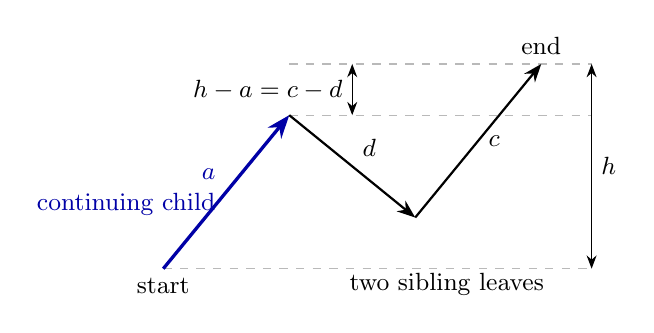
\begin{tikzpicture}[x=.8cm,y=.65cm,font=\small,>=Stealth]
 \draw[gray!55,dashed] (0,0)--(6.8,0);
 \draw[gray!55,dashed] (2,3)--(6.8,3);
 \draw[gray!55,dashed] (2,4)--(6.8,4);
 \draw[very thick,blue!65!black,->] (0,0)--(2,3)
   node[midway,left,align=right] {$a$\\continuing child};
 \draw[thick,->] (2,3)--(4,1) node[midway,above right] {$d$};
 \draw[thick,->] (4,1)--(6,4) node[midway,right] {$c$};
 \draw[<->] (6.8,0)--(6.8,4) node[midway,right] {$h$};
 \draw[<->] (3,3)--(3,4) node[midway,left] {$h-a=c-d$};
 \node[below] at (0,0) {start};
 \node[above] at (6,4) {end};
 \node[below,align=center] at (4.5,.1) {two sibling leaves};
\end{tikzpicture}
\caption{A unary expansion with the first child continuing. The parent
and child heights obey $h=a-d+c$, so a small continuing-height drop
forces the two sibling leaves to have nearly equal heights. If the
retreat continues instead, $a,c\in[d,h]$ and $|a-c|\le h-d$.
Only heights are represented: the horizontal spacing and straight
segments are schematic.}
\label{fig:11-sibling-heights}
\end{figure}

For a fixed path $\gamma$, let $K_\gamma$ be the probability law of
all these independent trial choices, over every eligible root subarc
and every potential descendant node. This is a finite product: the
path has at most $CH^2$ steps and all trees have depth at most $L$.
For a trial outcome $\omega$, let $N^{\mathfrak t}_{r,k}(\gamma,\omega)$
count the witnesses of kind $\mathfrak t\in\{\mathrm{spine},\mathrm{mark}\}$
with $k$ expansions and root span in $[r,2r)$. Different root subarcs
and different retained subtrees are counted separately. The weighted
witness mass is therefore
\[
 \int N^{\mathfrak t}_{r,k}(\gamma,\omega)\,
       K_\gamma(d\omega)\,\mu_H(d\gamma).
\]
In particular, a bound on this integral bounds the mass of path-and-trial
pairs having at least one such witness.

\smallskip\noindent\emph{Why these witnesses suffice.}
Suppose that the thin-excursion exception of
Lemma~\ref{lem:11-thin-excursions}, with $\lambda=\epsilon$, is absent,
and that a trial outcome contains neither kind of witness, for any
eligible root. If
\[
 pU^{-4/3}<1/4,
\]
then, for all sufficiently large $H$, every weak-bridge subarc $\sigma$
of span $s$ satisfies
\begin{equation}
 |\sigma|\le H^{2\epsilon}(1+s)^{4/3}.
 \label{eq:11-no-witness-length}
\end{equation}
This implication is deterministic; it holds for every outcome of the
trial choices.

Prove it by induction on three times the band span, an integer for
both vertex and horizontal-port endpoints. Below $H^\beta$ the thin
bound gives length at most $H^\epsilon$. For a larger root span $s$,
take its trial tree and prune at each non-long piece. At any depth
fewer than $p$ long pieces remain, since they are incomparable and
would otherwise give a marked witness. Thus at most $1+3pL$ non-long
pieces stop the pruning. Every long terminal piece has span below
$s/U$: a terminal at depth $L$ would give a spine. These long terminals
are also incomparable, so there are fewer than $p$ of them. Their
spans are strictly smaller than $s$, and the induction hypothesis
and exact length additivity give
\[
 |\sigma|\le (1+3pL)H^\epsilon(1+s)^{4/3}
       +pH^{2\epsilon}(1+s/U)^{4/3}.
\]
After division by the right-hand side of
\eqref{eq:11-no-witness-length}, the coefficient is
\[
 (1+3pL)H^{-\epsilon}
 +p\left(\frac{1+s/U}{1+s}\right)^{4/3}<1
\]
for large $H$, uniformly over $s\ge H^\beta$. This proves the
induction. It remains to show that the weighted mass of the two
witness classes is small.

\begin{lemma}[Turning-chain witness bound]\label{lem:11-chain}
There are absolute $b>0$ and $C<\infty$ such that, for fixed
$\epsilon,p,U$ and a root-span dyad $s\in[r,2r)$ with
$H^\beta/2\le r\le C_0H$, the weighted witness mass just defined is at most
\begin{equation}
 H^{C+o_{p,U,\epsilon}(1)}H^{-\epsilon m_*}
 \bigl[C'(1+\log\log H)^{C'}\bigr]^k(k+1)^{-bk}.
 \label{eq:L-39}
\end{equation}
There $m_*=0$ for a spine and $m_*=p$ for a
marked witness. The exponent
$C$ is independent of $p,U,\epsilon$; the constant $C'$ may depend on
them. The $o(1)$ is uniform in the indicated $r,k$, and denotes a
quantity tending to zero for those fixed parameters. The same bound,
with $m_*=0$ and $k$ equal to the number of pieces, holds for an
alternating chain of $1\le k\le pL$ pieces of nonincreasing spans in
$[r,2r)$, where $L=\lceil\log H\rceil$ and $p$ remains fixed.
For this last assertion the mass is the analogous sum over all
rooted chain records, without trial probabilities.
\end{lemma}

\begin{proof}
\emph{Cuts and bridge weights.}
We first record the cuts and relative bridge shapes. The calculation
then separates end tests from the remaining height variables. The
height restrictions are summed by bounds uniform in the end data, so
the tests can be integrated with their original renewal laws.

Every outer child of an expansion has span at least one third
of its parent's span. Choose $0<c_0\le1/(12U)$. Every expanded parent
has span at least $s/U\ge r/U$, so all leaves have spans between
$c_0r$ and $2r$, except possibly retreat leaves.
There are only $O_{p,U}(1)$ small retreat leaves, and they are isolated
between macroscopic leaves. To see the bound, the minimal witness has
$O(p)$ branching or terminal expansions and otherwise consists of
$O(p)$ unary chains. If a parent has height $h$ and a small retreat
has height $d<c_0r$, the middle-third cut gives both forward heights
at most $2h/3+d\le3h/4$. The retreat itself has height below $s/U$
and cannot continue.
Along a continuing chain heights never increase and stay at least
$s/U$ until the last expansion; there can consequently be only
$O_U(1)$ such reductions on each chain.
The first and last leaves of an expanded subtree descend through
outer children and are macroscopic, so small retreats are isolated
in the chronological leaf order.

Bin each small span plus one dyadically with scale $r_i$, and put
$r_i=r$ on macroscopic leaves. Fix the complete leaf pieces and all
cut records. At the parent of a small retreat, the chosen middle-third
line must belong to that retreat's height interval (one specified line
when it is empty); there are $O(r_i)$ possible choices out of at least
$cr$. Each small leaf therefore contributes $Cr_i/r$ to the probability
of these witness data. All other line-choice probabilities sum to at
most one. This uses only choices recorded by the witness, without
specifying any descendants outside it.

At a turn whose incident spans are both larger than $Cr^{1/20}$,
recode its incident leaves to strict bridges from neighboring ports,
preserving disjoint first-hit portions to distance
$c_A\min(r_i,r_{i+1})$. Here $c_A$ is small depending on $c_0$.
For completeness, at a peak both lower neighbors of its triangle occur
on the path. One arm uses the central top port. Launch the other from
the adjacent top port through the neighboring downward triangle to
its original lower neighbor. If that neighboring triangle already
occurs on this arm, it must occur immediately next to that lower
neighbor, so shorten the initial segment instead. An internal visit
would have to use the same lower neighbor. The other arm cannot use
this triangle in the retained first-hit portion for the same reason.
Reflect this operation at minima. Remote-end changes lie beyond the
retained first-hit portions. Where no turn test is required, extend
to bounding port lines; if an extreme triangle does not border that
line, one extra triangle nearer the line is unused by extremality.
Empty leaves have bounded bookkeeping. This gives a finite record
per cut and changes lengths and spans by $O(1)$.

After fixing those records, normalized bridge shapes have their
translations fixed successively by incidence. There is no additional
sum over horizontal positions at each turn. A turn test involves only
two relative shapes launched at fixed neighboring ports; changing
absolute translations does not change the test. The root location,
the two exterior portions, and endpoints cost $O(H^C)$ altogether by
the full-box bound, with $C$ independent of the number of leaves.

Baseline leaf $i$ by $r_i^\alpha$ and initially seek
$\min(r_i,r_{i+1})^{-\alpha}$ at every turn. Because small leaves are
isolated, multiplying the baselines, these turn factors, and the
placement probabilities gives at most
\[
 C^k r^\alpha\prod_{i\text{ small}}(r_i/r)^{1-\alpha}.
\]
If $r_i\le Cr^{1/20}$, omit both adjacent turn tests. Restoring their
nominal factors multiplies this expression by at most $Cr_i^{2\alpha}$.
The resulting contribution from that leaf is bounded, since
\[
 (r_i/r)^{1-\alpha}r_i^{2\alpha}
 \le C r^{-(1-\alpha)+(1+\alpha)/20}.
\]
No probes are needed at its own ends. Call turns touching small or
marked leaves \emph{rough}; there are $O_{p,U}(1)$ of these. All other
turns are \emph{ordinary}.

\smallskip\noindent\emph{End probes at ordinary turns.}
The factors at turns will cancel all but one of the bridge mass scales.
Their dependence on $k$ must remain explicit, because $k$ can be of
order $\log H$.

For a non-tiny leaf inspect its two strings of irreducibles through
the first renewals reaching
\[
 q_i=\left\lfloor c_qr_i(k+1)^{-\delta}\right\rfloor,
\]
with a sufficiently small fixed $\delta>0$. The coefficient $c_q$ is
small, and common on macroscopic leaves. For large $H$ these are
positive. The strings are of type $\mathrm M$ when disjoint, allowing
a common terminal cut, and then leave a free middle bridge. Otherwise
they share exactly one irreducible and have type $\mathrm Z$. Call an
end good when its stop lands below $c'r_i$, and bad otherwise, with
$c_q\ll c'\ll c_Ac_0$. In type $\mathrm Z$ both ends are bad.
A bad string is a prefix with endpoint depth below $q_i$, followed by
a jump of height comparable to $r_i$. For a birth dyad $f$, its prefix
cost is $Cf^\alpha$ and its jump cost is $Cr_i^{-\alpha}$. On an
$\mathrm M$ leaf the residual middle supplies baseline $r_i^\alpha$;
on a $\mathrm Z$ leaf its single shared jump supplies
$r_i^\alpha(r_i^{-\alpha})^2=r_i^{-\alpha}$. This equality is only
bookkeeping: every distinct shared jump is integrated once.
For example, among $n_0=m_0+z_0$ macroscopic pieces with $b_0$ bad
ends there are $d_{\mathrm{bad}}=b_0-z_0$ distinct bad jumps, and
\[
 r^{\alpha n_0}r^{-\alpha b_0}
       =r^{\alpha m_0}r^{-\alpha d_{\mathrm{bad}}}.
\]
The right-hand side records the genuine independent middle and jump
variables; the left-hand side assigns their costs to leaves and turns.

At an ordinary turn the desired estimates, beyond these leaf
baselines, are
\begin{equation}
\begin{array}{c|c}
 \text{incident ends}&\text{turn factor}\\ \hline
 \mathrm{GG}&Cr^{-\alpha}(k+1)^{\delta\alpha}\\
 \text{one good, one bad}&Cr^{-\alpha}\\
 \text{two bad}&Cr^{-\alpha}(k+1)^{-\delta\alpha}.
\end{array}
\label{eq:L-38}
\end{equation}
The total additional loss over all ordinary turns will be at most
$C^k(1+\log\log H)^{Ck}$.

First fix the birth dyads. Apply the ordered test $E$ from
\eqref{eq:T-34} at a small fraction of the minimum of the available
depths, using $q_i$ at a good end and $f$ at a bad end. At bounded
minimum use the trivial test. Its stopping renewals occur before the
first-hit portions terminate: on a bad end they precede the specified
birth, and a good stop is below $c'r$. Renewal cuts prevent later
visits below the tested level. Moreover two disjoint crosscuts from
the neighboring launches to the common first-hit line have the
required left--right extremal order at each lower level; a point past
the opposite extremum would lie on the wrong exterior side of that
crosscut. Hence $E$ is a necessary condition. After these stops the
remaining birth counts are at most $Cf^\alpha$, including the
possibility that the birth occurs at the stop itself. The three costs
for fixed dyads are respectively
\[
 Cq^{-\alpha},\qquad
 Cr^{-\alpha}f^\alpha\min(f,q)^{-\alpha},\qquad
 Cr^{-2\alpha}f^\alpha g^\alpha\min(f,g)^{-\alpha}.
\]
Since $f,g\le Cq$ these give the table; the last expression is more
precisely $Cr^{-\alpha}(\max(f,g)/r)^\alpha$.

\smallskip\noindent\emph{Summing birth depths.}
We must sum the birth dyads without a power of $\log H$ at every turn.
Set
\[
 t=\lfloor r(1+\log H)^{-D_*}\rfloor,\qquad
 T_0=r(1+\log H)^{-10},
\]
where $D_*>12$ is a sufficiently large fixed constant. Tag an unmarked
macroscopic bad jump if, from either of its relevant ends, it returns
to depth at most $2t$ after reaching $c''r$, where $c''>0$ is small.
By Lemma~\ref{lem:11-small-return}, choosing $D_*$ larger if necessary,
the mass of tagged jumps is
\[
 Cr^{-\alpha}(1+\log H)^{-5}.
\]
The constants are uniform for $H^\beta/2\le r\le C_0H$, since
$\log r\asymp_\beta\log H$. The union over two ends costs only a
constant, and no designated-jump test below will be assigned to a
tagged jump.

If both bad birth depths are at most $T_0$, sum their dyads using the
improved maximum factor. Summing over the larger dyad first gives
\[
 \sum_{f,g\le CT_0}\left(\frac{\max(f,g)}r\right)^\alpha
 \le C(1+\log H)(T_0/r)^\alpha
 \le C(k+1)^{-\delta\alpha},
\]
for small $\delta$, since $k\le pL$. Birth dyads between $t/L_2$ and
$Cq$ have only $O(1+\log\log H)$ possible values. Here $L_2$ is the
fixed paired-test constant in \eqref{eq:T-34}, unrelated to the trial
depth $L$. The remaining situation has a birth below $t/L_2$ opposite
a good end or a bad birth larger than $T_0$. If its jump is tagged,
sum this early birth dyad directly. A distinct jump has at most two
ends; its factor $(1+\log H)^{-5}$ pays both possible lost dyad sums,
each of size $O(1+\log H)$.

For an untagged jump in that remaining situation, use
$F(t,r',0)$ from \eqref{eq:T-34}, designating the early-birth end;
$r'$ is the jump's height dyad, with only a bounded number of choices
comparable to $r$. The opposite end supplies an independent worker
string. Its test stop precedes any specified bad birth there, since
that birth is above $T_0\gg t$. On the designated arc, every visit
below $t$ up through the jump occurs before the common first-hit line.
Otherwise, as the designated birth is below $t/L_2$, the jump itself
would reach $c''r$ and subsequently return below $2t$, forcing its tag.
The crosscut argument thus gives the required $E(t)$ event. If the
same jump is designated from both ends, use the single paired bound
$F_{12}(t,t,r')$ instead. It integrates that one jump, both early
prefixes, and both opposite workers' tests. In either case the cost
is $Cr^{-\alpha}$ for the distinct jump and all its designated
prefixes and tests. A worker with a later bad birth still contributes
$Cg^\alpha$ after its test, so a two-bad turn retains its factor
$(g/r)^\alpha\le C(k+1)^{-\delta\alpha}$. The single-test birth
condition holds because $L_2$ is at least the single-test ratio in
\eqref{eq:T-34}.

\smallskip\noindent\emph{Simultaneous integration.}
We will combine the turn gains with restrictions on residual middle
heights. The needed restriction can be stated now. For an unmarked
macroscopic $\mathrm M$ leaf, let $z$ be the combined height of its two
end strings and $j$ its middle height. Its total height is $z+j$.
The normalized middle kernel
\[
 K_r(j)=r^{-\alpha}B_j\mathbf1_{\{0\le j\le Cr\}}
\]
obeys, for every interval $I$ of width $w\ge1$ and every shift $z$,
\begin{equation}
 \sum_{j:\,z+j\in I}K_r(j)\le C(w/r)^\alpha.
 \label{eq:11-middle-window}
\end{equation}
Indeed $B_j\le C(1+j)^{\alpha-1}$, so the sum over any $w+1$
consecutive heights is at most $Cw^\alpha$. Since $k\le pL$ and
$r\ge H^\beta/2$, requiring
two leaf heights to differ by $O(1+r/\sqrt{k})$ costs
$O((k+1)^{-\alpha/2})$ if one leaf is of type $\mathrm M$: fix the
partner's height, sum that middle in its translated window, and then
sum the partner's middle freely if it has one. The bound is uniform
in the partner's end strings and jumps, leaving those variables
available for their later probe estimates. For disjoint leaf pairs
these middle integrations can be performed together.
The construction of sufficiently many such pairs is given below.

We now integrate the turn tests while retaining these uniform
middle-height gains. Work with nonnegative critical-weight sums and
fix only discrete records: the chain shape, scales, piece types,
good/bad labels, tag labels, and assignments of turn tests. Do not
condition any bridge law on its total height or on the completed
chain. For an $\mathrm M$ leaf its atomic variables are its two
oriented end prefixes, any distinct bad stopping jumps, and its
middle bridge. For a $\mathrm Z$ leaf they are the two pre-jump
prefixes and one shared jump. Concatenation identifies a tuple of
such variables with at most a constant number of original records.
Dropping unused self-avoidance and incidence conditions therefore
bounds the original sum by a product of their critical measures.
The restrictions retained in this product are local turn tests,
individual jump restrictions, and the residual-height constraints
just described.

Each end prefix occurs at exactly one turn, or at a free chain end.
Assign every distinct bad jump to exactly one of three blocks: its
individual tail bound (with its tag restriction if present), a
single $F$ block, or a paired $F_{12}$ block. A designated block
contains the designated pre-jump prefix or prefixes and the opposite
worker prefixes through their test stops. An ordinary $E$ block
contains its two prefixes only through their test stops. These sets
of variables are disjoint. In particular a worker at a designated
turn has no early designated birth there: it is either good or its
birth is above $T_0$. The tested worker portion therefore excludes
its own separately charged bad jump. If a shared jump has just one
assigned $F$ test, the test at its other end uses only the prefix
before that jump; it belongs to a different block and never uses
the shared jump a second time.

First sum the residual middles with the prescribed height
restrictions, using \eqref{eq:11-middle-window} for one middle in
each disjoint pair and the unrestricted bound for the others.
These bounds are uniform in all the end variables. Leave every designated
pre-jump prefix intact inside its assigned $F$ or $F_{12}$ block.
For an ordinary $E$ prefix or a worker prefix, next sum only its
untested continuation. Given its test stopping history,
the mass of subsequent renewal occurrences in a birth dyad $g$ is
at most $Cg^\alpha$, uniformly in the stopping location and overshoot:
an overshoot beyond the permitted endpoint contributes zero, and
otherwise the remaining range has length at most $Cg$. A good
completion is a probability at most one. Length insertions are
handled by the same conditional argument described below. Replacing
these continuation sums by their uniform bounds removes them without
conditioning the preceding tests. Now integrate each disjoint $E$,
$F$, or $F_{12}$ block using \eqref{eq:T-34}; integrate every remaining
jump using its individual tail bound. Tonelli's theorem justifies this
order. Relative launches in each block are fixed neighboring ports,
so absolute translations depending on variables outside the block
introduce no parameter into its estimate. In a paired block this is
exactly the two-end convention in the definition of $F_{12}$.
Finally sum the discrete labels and dyads as above. Thus no estimate
has been applied to a renewal law conditioned on an eventual height,
a tag, another turn's survival, or full-chain avoidance. This proves
\eqref{eq:L-38} with the stated total loss.

\smallskip\noindent\emph{Long marked leaves.}
The ordinary-turn estimates control the unmarked chain. A marked leaf
must additionally pay $H^{-\epsilon+o(1)}$ for exceeding its length
threshold. Only a fixed number of turns touch such leaves, so the
logarithmic first-hit estimate suffices there.

We next include rough turns and the marked length factors. Uniformly
for $1\le u\le C H$, the first-length moment gives
\[
 \sum_{j\le Cu}\sum_{B:\,\operatorname{ht}(B)=j}
       \rho^{|B|}(1+|B|)
 \le u^{\alpha+4/3}H^{o(1)}.
\]
The analogous summed moment for an irreducible of height at most $Cu$
is at most $u^{4/3-\alpha}H^{o(1)}$. Indeed, in a height dyad $b$,
prepend and append bridges of heights in $[b,2b]$, whose summed
masses each are at least $cb^\alpha$. The resulting bridge has height
$O(b)$ and has only boundedly many irreducibles of height at least $b$.
Its length moment bounds the marked jump's length moment, giving
$b^{4/3-\alpha}H^{o(1)}$ after division by $b^{2\alpha}$.
Sum the dyads, using $4/3>\alpha$. These moment statements mean that
for every fixed $\eta>0$ the displayed factors $H^{o(1)}$ are bounded
by $C_\eta H^\eta$, uniformly over all indicated scales.

Expand the product of length-plus-one factors on marked leaves by
assigning each insertion to its middle, a bad jump, a good end string,
or a pre-bad-jump prefix. There are only boundedly many categories
per marked leaf; for an end string sum over its individual jumps.
A middle or tiny-piece insertion costs at most
$r_i^{4/3}H^{o(1)}$ beyond its unweighted baseline. A bad-jump insertion
has the same relative cost by the irreducible moment. No tag saving
or designated $F$ test uses a marked leaf's own jump.

For an insertion in an end string, let $d$ be the dyadic scale of one
plus the inserted jump's birth depth. Up to that birth the occurrence
mass is at most $Cd^\alpha$. The jump's length moment, after extracting
$r_i^{4/3}H^{o(1)}$, costs $Cr_i^{-\alpha}$. Thus this insertion gives
an additional factor $(d/r_i)^\alpha$. Any subsequent required bad
birth of dyad $f$ costs at most $Cf^\alpha$ by restarting after the
inserted jump, with its bad-jump price already separately budgeted;
completion to a good stop has probability at most one. This includes
the terminal stopping jump of a good string. Additive constants in
the length weight use the unweighted estimate.

At a non-omitted rough turn apply the first-hit bound
\eqref{eq:T-35a} at a small fraction of the smaller available depth.
Use $d$ on an end with an insertion in its prefix, $f$ on another bad
end, and $q_i$ on another good end. The test precedes the counted
births and lies within the preserved disjointness range. Subsequent
occurrence counts have the same conditional bounds as before. A
side of available depth $v$ has, after extraction of its baseline
and any length price, cost at most
$H^{o(1)}(v/r_i)^\alpha$. For a good side the factor is supplied at
polylogarithmic cost, since $q_i/r_i$ is a negative power of $k+1$.
For two incident sides the test and these factors give
\[
 H^{o(1)}\frac{v_1^\alpha v_2^\alpha}
                   {r_i^\alpha r_{i+1}^\alpha}
             \min(v_1,v_2)^{-\alpha}
 \le H^{o(1)}\min(r_i,r_{i+1})^{-\alpha},
\]
because $v_j\le Cr_j$. Free ends and omitted turns cost at most
$H^{o(1)}$. There are only $O_{p,U}(1)$ rough turns and small leaves.
Their scale choices cost $(1+\log H)^{O_{p,U}(1)}$, so all these losses
remain $H^{o_{p,U}(1)}$.

This rough calculation is compatible with the preceding block
integration. At a rough turn an unmarked neighboring leaf supplies
only its good prefix or its prefix before a bad jump; no marked
insertion or rough test consumes that unmarked bad jump. Stop the
rough tests before the inserted jumps, then use the conditional
moment and renewal bounds for the continuations. Distinct marked
leaves have distinct inserted jumps. Their length prices hence
multiply. On a long marked leaf,
\[
 \mathbf 1_{\{|B|>H^\epsilon(1+\operatorname{ht}(B))^{4/3}\}}
 \le \frac{1+|B|}{H^\epsilon(1+\operatorname{ht}(B))^{4/3}}.
\]
Its scale is comparable to $1+\operatorname{ht}(B)$, so division by
this threshold gives $H^{-\epsilon+o(1)}$ per mark.

\smallskip\noindent\emph{The gain from many leaves.}
We have obtained the turn baselines and the cost of each marked
length. It remains to obtain the factor $(k+1)^{-bk}$ from the many
unmarked macroscopic leaves. We now construct the close-height pairs
to which \eqref{eq:11-middle-window} applies.

There are disjoint sibling pairs covering all but
$O_{p,U}(\sqrt{k}+1)$ leaves for which the two leaf heights differ by
$O(1+r/\sqrt{k})$. Indeed all but $O(p)$ expansions lie on unary
chains. The total drop of continuing heights along each such chain
is at most $2r$, so at most $O(\sqrt{k})$ expansions on that chain
have a drop larger than $r/\sqrt{k}$. At every other unary expansion
the two non-continuing children are
leaves. Write $h$ for the parent height, $a,c$ for the forward child
heights, and $d$ for the retreat height. The signed-height identity is
$h=a-d+c$, and all three child heights are at most $h$.
If the first child continues, the drop $h-a=c-d$ is exactly the
difference of the other two heights; the last-child case is symmetric.
If the retreat continues, then $a+c=h+d$, with $a,c\le h$, so
$a,c\in[d,h]$ and $|a-c|\le h-d$. Consequently a continuing-height
drop at most $r/\sqrt{k}$ always supplies a sibling pair whose heights
differ by at most that amount, up to the bounded port recodings. Remove
the boundedly many pairs touching marked or small leaves. Specifying
which of these pairs meet the constraint and their types costs at
most exponentially many choices in $k$.

In each retained pair with at least one $\mathrm M$ leaf, integrate
one such middle kernel with the height constraint, holding the
partner's height fixed. If the partner also has a middle, sum that
middle without the constraint. The pairs
are disjoint, so these integrations are simultaneous and uniform in
all probe variables. These are the residual integrations used in
the block argument above. There are $N=2k+1$ leaves. If at least $N/10$ are $\mathrm M$,
then, after removing the $O_{p,U}(\sqrt{k}+1)$ exceptions, at least
$N/40$ retained pairs contain an $\mathrm M$ leaf for large $k$.
Their total gain is at most $(k+1)^{-\alpha N/80}$. The at most $N$
good--good turns cost at most $(k+1)^{\delta\alpha N}$, so a fixed
choice $0<\delta<1/160$ leaves a negative multiple of $k\log(k+1)$.
If fewer than $N/10$ leaves are $\mathrm M$, at least
$4N/5-1-O_{p,U}(1)$ adjacencies join two $\mathrm Z$ leaves,
allowing for the bounded number of small leaves and rough exceptions. At most $N/10$ adjacencies can be good--good.
For large $k$ the excess of bad--bad over good--good ordinary turns
is therefore at least $N/2$, giving the factor
$(k+1)^{-\delta\alpha N/2}$.
Thus in either case the total factor
is at most $(k+1)^{-bk}$ for an absolute $b>0$, apart from constants
to the power $k$ and the stated logarithmic losses. Bounded $k$ are
absorbed by changing the constants.

Ordered ternary tree shapes, choices of the continuing children,
piece labels, and the finite recoding records have at most
exponential multiplicity in $k$. Choices of the fixed number of
marks contribute $H^{o_p(1)}$. Small-scale dyads do so as well. The
factor $r^\alpha$, root placements and exterior paths are all covered
by a fixed polynomial $H^C$ independent of $p,U$. This proves the bound in \eqref{eq:L-39}.

For the final assertion of the lemma, start instead with the given
alternating chain of $k\le pL$ comparable, nonincreasing spans. This
range preserves the probe and dyad estimates above. There are no
small leaves or placement weights. Pair successive pieces, leaving
at most one unpaired. Since the total height drop is at most $2r$,
all but $O(\sqrt{k})$ pairs have difference at most $Cr/\sqrt{k}$.
The same recoding, tests, variable partition, and middle-kernel
integrations apply, and give the stated estimate.
\end{proof}

\subsection{Slow-path amplification}

\begin{proof}[Proof of Theorem~\ref{thm:11-local-length}]
Choose $\epsilon>0$ much smaller than $\tau$. In the notation of
Lemma~\ref{lem:11-chain}, when $k=L$ the logarithm of the last two
factors of \eqref{eq:L-39} is
\[
 -bL\log L+O\bigl(L\log(2+\log\log H)\bigr),
\]
which is smaller than $-A\log H$ for every fixed $A$ and all
sufficiently large $H$. Thus spine witnesses have superpolynomially
small mass. For arbitrary $k\le pL$, let
$V_H=C'(1+\log\log H)^{C'}$. The maximum of
$k\log V_H-bk\log(k+1)$ is $O(V_H^{1/b})=o(\log H)$.
Consequently the sum over $k$ costs $H^{o(1)}$. Choose $p$ sufficiently
large that the factor $H^{-p\epsilon}$ absorbs the fixed polynomial
and the desired failure power. Next choose $U$ large enough that
$pU^{-4/3}<1/4$. Constants depending on these now fixed parameters
do not affect either conclusion. Summing the $O(\log H)$ root dyads
makes all unwanted witnesses negligible at any prescribed power.

Sum the witness bounds over their sizes and use the kernel
$K_\gamma$ defined above. Since each witness count dominates its
existence indicator, the resulting bound controls the
$\mu_H(d\gamma)K_\gamma(d\omega)$-mass of pairs containing any unwanted
witness. The root-subarc choices are already included in that count.
Add the path exceptional set from
Lemma~\ref{lem:11-thin-excursions}, with parameter $\lambda=\epsilon$.

Every remaining path-and-trial configuration satisfies the
deterministic implication \eqref{eq:11-no-witness-length}.
That weak-bridge statement is a property of $\gamma$ alone.
If a path violates it and is not in the thin exceptional set, every
trial configuration over that path must contain an unwanted witness.
Therefore, writing $\mathcal B$ for the bad paths and $\mathcal W$
for the unwanted configurations,
\[
 \mu_H(\mathcal B)
 =\int_{\mathcal B}K_\gamma(\Omega_\gamma)\,d\mu_H(\gamma)
 \le (\mu_H K)(\mathcal W)
       +\mu_H(\text{thin-excursion exception}).
\]
There is no loss from projecting away the trial variables.

To pass to arbitrary subwalks, split at a lowest vertex and read both
halves away from that vertex. Successively cut each half at the last
alternating extremum of the remaining tail. This gives weak bridges
of nonincreasing spans. Outside another superpolynomial exceptional
set, there are fewer than $\lceil\log H\rceil$ consecutive pieces in
any one span dyad above $H^\beta/2$: otherwise apply the final part
of Lemma~\ref{lem:11-chain} to $k=L=\lceil\log H\rceil$ of those
pieces. Root locations and
exterior pieces again have only fixed polynomial cost. Summing the
weak-bridge length bound over decreasing dyads gives at most
$CH^{2\epsilon}\log H(1+s)^{4/3}$ per half. Once the remaining span is
below $H^\beta$, the whole remaining tail is thin and has length at
most $H^\epsilon$. Choose $\epsilon$ so that these bounds fit
$H^\tau(1+s)^{4/3}$ for large $H$. Enlarging the exceptional-set
constant handles bounded $H$. A finite union over lattice symmetries
proves the simultaneous directional statement.
\end{proof}

\subsection{Many crossings}

We use the all-count cylinder estimate stated among the analytic
inputs. For clarity, its precise physical form is the following: on
the balanced two-marker cylinder with $N=2m$ bands, the first $m$ band
parameters are $2\lambda$ and the next $m$ are $\lambda$. If $w_N(a)$
is the critical mass of families of exactly $a$ mutually disjoint
polygons separating the markers, then
\begin{equation}
 w_N(a)\le
 \exp\!\left(C\log N-\frac{ca^2}{\log N}\right)
 \qquad(a\ge0)
 \label{eq:L-40}
\end{equation}
for every sufficiently large even $N$, with one pair of constants
independent of $N$ and $a$. The analytic input proves, before sector
truncation, $Z_N(2\cosh v)\le\exp(C\log N(1+v^2))$ for every
$v\ge0$; positivity and optimization in $v$ give
\eqref{eq:L-40}. The quantifier over all $a$ is needed below, since
the number of crossings grows as a power of the ambient scale.

\begin{lemma}[Many bridges in one slab]\label{lem:11-many-bridges}
Fix $D<\infty$. Consider ordered tuples of $a$ mutually avoiding
strict bridges across the same $j\ge1$ bands, all contained in one
abscissa slab of width $Dj$. Prescribe the distinct starting ports,
the distinct ending ports, and their matching. The critical mass of
these tuples is at most
\begin{equation}
 \exp\!\left(C_D\log(2+j)-\frac{c_Da^2}{\log(2+j)}\right).
 \label{eq:L-41}
\end{equation}
\end{lemma}

\begin{proof}
Put $d_0=\sqrt3/2$ and use triangular coordinates with generators
$(1,0)$ and $(1/2,d_0)$. Choose a fixed integer $b=b(D)$ sufficiently
large and put $m=bj$. In the physical cylinder the successive half-period
translations are
\[
 m(-1/2,d_0),\qquad m(1/2,d_0).
\]
Thus the total period is $(0,2md_0)$ and the marker abscissas differ
by $m/2$. For $b$ sufficiently large, an integer horizontal translation
places the entire width-$Dj$ slab strictly between those abscissas,
with a fixed positive margin. Align its bottom with a marker band level.

Label the fixed lower ports $s_1,\ldots,s_a$ and the fixed upper
ports $t_1,\ldots,t_a$, and write $\pi$ for the fixed matching:
strand $i$ joins $s_i$ to $t_{\pi(i)}$. Choose independently $2b$
tuples from the ensemble. Put the first in bands $0,\ldots,j$ and
reflect the second across the line at height $jd_0$, traversing it
upward. Reflection across any horizontal band boundary is a lattice
symmetry. The second strip takes $t_{\pi(i)}$ to the translate of
$s_i$ at height $2jd_0$. Repeat this construction in successive double
strips. Each double strip therefore induces the identity on the lower
port labels. After all $2b$ strips, the vertical quotient closes each
strand at its own initial port.

The strip interiors are disjoint. Strict bridges meet their boundary
cuts only at the fixed ports, and those ports are distinct within each
tuple. Hence the resulting family contains exactly $a$ disjoint simple
polygons. Each lift travels through one full vertical period, so each
polygon is essential. Since the whole family stays between the marker
abscissas, each polygon separates the two markers.

Cutting this family at the fixed $j$-spaced levels recovers every input
tuple. The strip index specifies its reflection, and the prescribed
ports recover the strand labels and matching. Recovery is therefore
injective even though the polygon family itself is unlabeled and
unoriented. Ports carry no vertex weight, so the critical weights
multiply exactly at every concatenation. If $M$ is the input tuple
mass, positivity and \eqref{eq:L-40} give
\[
 M^{2b}\le w_{2bj}(a)
 \le\exp\!\left(C\log(2bj)-\frac{ca^2}{\log(2bj)}\right).
\]
Take the $2b$th root and use
$\log(2bj)\asymp_b\log(2+j)$. For bounded $j$, the fixed-width slab
contains only boundedly many distinct ports, so $a$ is bounded;
the finite bridge masses cover these cases by changing the constants.
\end{proof}

\subsection{Local vertex mass and the temporal modulus}

\begin{proposition}[Uniform local mass bound]\label{prop:11-local-mass}
For every $\tau>0$ and $A>0$, there is $C_{\tau,A}<\infty$ such that
for all $H\ge2$, outside a set of $\mu_H$-mass at most
$C_{\tau,A}H^{-A}$, simultaneously for every visited vertex $v$ and
every real radius $1\le s\le H$,
\begin{equation}
 \#\bigl(V(\gamma)\cap\overline B(v,s)\bigr)\le H^\tau s^{4/3}.
 \label{eq:L-42}
\end{equation}
\end{proposition}

\begin{proof}
Use Theorem~\ref{thm:11-local-length} with a smaller slack $\tau'>0$.
It suffices to prove the statement at dyadic radii with further slack;
rounding a radius upwards then absorbs the constant for all radii.
There are polynomially many possible centers and $O(\log H)$ scales.
Small fixed radii are harmless by the lattice area bound.

For fixed $v,s$, surround $v$ by a lattice hexagonal box whose faces
are at perpendicular distances between $10s$ and $20s$. For each face
fix a parallel inner lattice line about $4s$ inward. Starting at the
next visit to $\overline B(v,s)$, follow the walk until its first subsequent hit
of a box face, or its endpoint; repeat at the next visit to the ball.
Each such visit batch is contained in the box. Its span is $O(s)$,
so the local length bound, with bounded trimming at face ports,
allows at most $CH^{\tau'}s^{4/3}$ visited vertices in that batch.
If \eqref{eq:L-42} fails, then for a fixed small
$0<\xi<\tau-\tau'$ and large $H$, at least
$a=\lceil H^\xi\rceil$ completed passages reach the same face.
There is at most one uncompleted terminal batch.

From each selected passage retain its segment from the last hit of
that face's inner line to the first hit of the face. These are
mutually disjoint strict bridges, all of height $j\asymp s$, in the
common box and hence a slab of width $Dj$, after a lattice symmetry.
If there are fewer than $a$ available ports, the event is empty.
Otherwise the endpoint tuples, matchings, and chronological placements have
at most $\exp(O(a\log H+\log H))$ choices. The complementary path
segments cost the same order: there are $a+1$ of them, each with
polynomial full-box susceptibility, and we may drop their mutual
avoidance. Apply Lemma~\ref{lem:11-many-bridges} to each fixed choice.
Since $s\le H$, the total mass is bounded by
\[
 \exp\!\left(Ca\log H+C\log H-\frac{ca^2}{\log H}\right),
\]
which is smaller than every power of $H^{-1}$ for $a=\lceil H^\xi\rceil$.
The polynomial union over centers and scales, and the exceptional
set for the local length estimate, preserve the claim.
\end{proof}

\begin{proposition}[Uniform temporal modulus]\label{prop:11-modulus}
For every $\tau>0$ and $A>0$ there is $C_{\tau,A}<\infty$ such that,
for every $H\ge2$, outside a set of $\mu_H$-mass at most
$C_{\tau,A}H^{-A}$, every subwalk $\sigma$ of $l$ steps satisfies
\[
 \operatorname{diam}(\sigma)\le H^\tau(1+l)^{3/4}.
\]
\end{proposition}

\begin{proof}
A violation has diameter $d>H^\tau(1+l)^{3/4}$. Some lattice normal
projection has span at least $cd$. Between its extreme levels take
an intervening weak bridge and extend it to a strict bridge. Its
height $h$ is at least $cd$ and at most $CH$, and its length is at
most $l+O(1)$. Thus $h\ge cH^\tau$ and, for a smaller fixed
$\tau'>0$ and large $H$,
\[
 l+O(1)\le C H^{-4\tau/3}h^{4/3}\le h^{4/3-\tau'}.
\]
Apply the fast-bridge estimate \eqref{eq:F-33b} dyadically in $h$.
The height lower bound is a positive power of $H$, and all placements
and exterior portions cost only a fixed polynomial by the full-box
bound. Its arbitrary failure power therefore gives the assertion.
\end{proof}

\section{Completion of the fixed-length theorem}\label{sec:fixed-length}
We now collect the consequences of the full-box estimates. This also identifies exactly where their unnormalized statements become probability estimates at a specified length.

\subsection{The probability transfer}
Let \(Z_n=c_n\rho^n\) be the critical partition function of the
\(n\)-edge paths from the fixed root.
\begin{lemma}[Normalization at every length]\label{09_fast_paths:normalization}
For every integer \(n\ge0\),
\begin{equation}\label{eq:normalization}
 Z_n\ge1.
\end{equation}
\end{lemma}
\begin{proof}
The honeycomb lattice is vertex-transitive. Cutting a walk after \(m\)
edges and forgetting the mutual avoidance of its two pieces gives
\(c_{m+n}\le c_mc_n\). If \(Z_{n_0}=a<1\) for some positive
\(n_0\), writing \(n=qn_0+r\), \(0\le r<n_0\), gives
\[
 Z_n\le a^q\max_{0\le r<n_0}Z_r\le Ce^{-cn}.
\]
Trimming the two endpoint half-edges of a port bridge gives a vertex
walk from one of finitely many possible neighbors of the source port;
the weight ratio and inverse multiplicity are bounded. A height-\(h\)
bridge has at least a constant multiple of \(h\) edges. The preceding
bound would therefore imply
\(B_h\le C\sum_{n\ge c'h}e^{-cn}\le C'e^{-c''h}\), contrary to
\(B_h\asymp h^{-1/4}\). The zero-length case is immediate.
\end{proof}

Every $n$-step path from $o$ lies in a Euclidean ball of radius a constant times $n$. Choose the full-box scale $H=Kn$, with a fixed $K$ large enough to contain that ball and the bounded port extensions used in cutting. The distinction between the critical edge and vertex weights at those extensions costs a bounded factor. If a bad collection in this full box has unnormalized critical mass at most $C_AH^{-A}$, then its subset of length $n$ has $\Prob_n$-probability at most
\[
 \frac{C_AH^{-A}}{Z_n}\le C_AH^{-A}.
\]
Thus arbitrary polynomial decay in $H$ is preserved at \emph{every} length. There is no averaging over lengths in this step.

For convenience we record the three simultaneous consequences used below. For every $\eta>0$ and $k>0$, outside an event of probability $O_{\eta,k}(n^{-k})$, all subwalks $\gamma[i,j]$ and all visited centers satisfy
\begin{align}
 j-i&\le C n^\eta(1+\diam\gamma[i,j])^{4/3},\label{eq:reduction-slow}\\
 \diam\gamma[i,j]&\le C n^\eta(1+j-i)^{3/4},\label{eq:reduction-fast}\\
 M_\gamma(z,s)&\le C n^\eta s^{4/3}\quad(1\le s\le n).
 \label{eq:reduction-mass}
\end{align}
Here \eqref{eq:reduction-slow} follows from the slow-path estimate \eqref{eq:L-37}, since a directional span is bounded by the Euclidean diameter. Equation~\eqref{eq:reduction-fast} is Proposition~\ref{prop:11-modulus}, deduced from \eqref{eq:F-33b}. Equation~\eqref{eq:reduction-mass} is \eqref{eq:L-42}. The constants $C$ and the fixed factor $K^\eta$ can be absorbed by a slightly larger exponent. Those statements already count all needed positions, directions, and scales in a full box; no independence of subwalks under $\Prob_n$ is asserted.

\subsection{Diameter and local mass}
\begin{proof}[Proof of Theorem~\ref{thm:main}]
Fix $\delta,k>0$. Use \eqref{eq:reduction-slow}--\eqref{eq:reduction-mass} with a positive $\eta$ much smaller than $\delta$ and with the prescribed failure exponent $k$. All arguments below take place on their single simultaneous good event.

Applying \eqref{eq:reduction-slow} to the entire path gives
\[
 1+D\ge c n^{(3/4)(1-\eta)}.
\]
Equation~\eqref{eq:reduction-fast}, again for the entire path, gives
$D\le Cn^{3/4+\eta}$. Taking $\eta$ small enough, then $n$ large enough, absorbs the constants and the additive one and proves \eqref{eq:main-diameter}.

For the upper local mass bound, use both the deterministic bound $M_\gamma(z,s)\le n+1$ and \eqref{eq:reduction-mass}. For sufficiently small $\eta$ and large $n$ this gives
\[
 M_\gamma(z,s)\le n^\delta\min\{n,s^{4/3}\}.
\]
To prove the lower bound, fix $z=\gamma_i$ and $s\in[1,n]$, and put
$m_0=\min\{n,s^{4/3}\}$. If $n^{-\delta}m_0\le1$, the vertex $z$ itself suffices. Otherwise choose
\[
 q=\left\lfloor n^{-\delta/2}m_0\right\rfloor.
\]
For large $n$, one side of $i$ has at least $n/2\ge q$ edges available. Choose the contiguous block of $q$ edges on that side. Since $m_0>n^\delta$, we have $q\ge\tfrac12n^{-\delta/2}m_0$ and $q+1\le2n^{-\delta/2}m_0$ for large $n$. Its diameter is at most
\[
 C n^\eta(1+q)^{3/4}
 \le C' n^{\eta-3\delta/8}m_0^{3/4}
 \le C' n^{\eta-3\delta/8}s\le s,
\]
provided $\eta<3\delta/8$ and $n$ is large. The entire block lies in $\overline B(z,s)$. Self-avoidance makes its $q+1$ vertices distinct, and
$q+1\ge n^{-\delta}m_0$ for large $n$. This proves the lower local mass bound simultaneously in $i$ and $s$, using only the already simultaneous modulus.

\subsection*{Covering numbers}
For a lower bound, consider any cover by $b$ balls of radius $s$. Discard balls missing $V(\gamma)$. In each remaining ball choose one visited vertex $z$. The visited vertices in that ball lie in $\overline B(z,2s)$. When $2s\le n$, the upper local mass estimate at $2s$, with smaller exponent slack, bounds their number by
\[
 Cn^\eta\min\{n,s^{4/3}\}.
\]
When $2s>n$, the deterministic mass bound $n+1$ gives the same conclusion after changing $C$. Summing over the covering balls gives
\[
 b\ge c n^{-\eta}\max\{1,ns^{-4/3}\}.
\]
Since $\max\{1,u\}\ge(1+u)/2$, constants and the smaller exponent slack imply the lower bound in \eqref{eq:main-cover}.

For the upper bound, fix a positive $\epsilon<\delta$ and put
$m_0=\min\{n,s^{4/3}\}$ as above. If $n^{-\epsilon}m_0<2$, use one ball for each vertex. The inequality $m_0<2n^\epsilon$ implies
\[
 n+1\le Cn^\epsilon(1+ns^{-4/3}).
\]
Otherwise let $q=\lfloor n^{-\epsilon}m_0\rfloor$. Split time into consecutive blocks of at most $q$ edges, allowing consecutive blocks to share one endpoint. Each block has diameter at most
\[
 C n^\eta(1+q)^{3/4}
 \le C' n^{\eta-3\epsilon/4}s\le s
\]
if $\eta<3\epsilon/4$ and $n$ is large. A ball of radius $s$ centered at a vertex in the block covers it. The number of blocks is at most
\[
 1+\frac n q\le C n^\epsilon(1+ns^{-4/3}).
\]
Taking $\epsilon<\delta$ absorbs the constant. The whole argument is deterministic on the good event, so the bounds hold simultaneously for all real radii in the stated range. This completes the proof.
\end{proof}

Figure~\ref{fig:covering} illustrates the two deterministic steps
that turn temporal and local-mass control into covering bounds.

\begin{figure}[htbp]
\centering
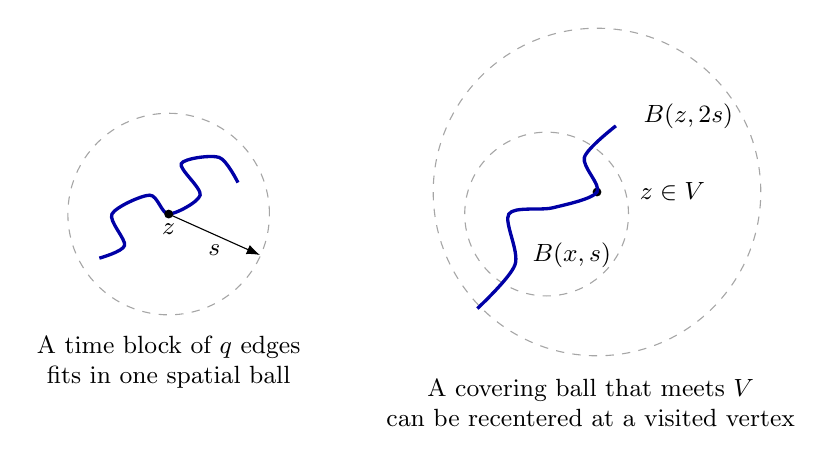
\begin{tikzpicture}[scale=.8,font=\small,>=Latex]
\draw[gray!70,dashed] (0,0) circle (1.6);
\draw[blue!65!black,very thick] plot[smooth] coordinates {(-1.1,-.7) (-.7,-.5) (-.9,0) (-.3,.3) (0,0) (.5,.3) (.2,.8) (.8,.9) (1.1,.5)};
\fill (0,0) circle (2pt) node[below] {$z$};
\draw[->] (0,0)--(1.45,-.65) node[midway,below] {$s$};
\node[align=center] at (0,-2.35) {A time block of $q$ edges\\fits in one spatial ball};
\begin{scope}[xshift=6cm]
\draw[gray!70,dashed] (0,0) circle (1.3);
\draw[gray!70,dashed] (.8,.35) circle (2.6);
\fill (.8,.35) circle (2pt) node[right,xshift=12pt] {$z\in V$};
\draw[blue!65!black,very thick] plot[smooth] coordinates {(-1.1,-1.5) (-.5,-.8) (-.6,0) (.1,.1) (.8,.35) (.6,.9) (1.1,1.4)};
\node at (.4,-.65) {$B(x,s)$};
\node at (2.25,1.55) {$B(z,2s)$};
\node[align=center] at (.7,-3) {A covering ball that meets $V$\\can be recentered at a visited vertex};
\end{scope}
\end{tikzpicture}
\caption{The two deterministic uses of local control. The modulus bounds the diameter of a contiguous block and yields the upper covering bound. The local mass upper bound, after recentering, yields the lower covering bound. The curves are schematic.}
\label{fig:covering}
\end{figure}

\begin{proof}[Proof of Corollary~\ref{cor:directional-span}]
The local-length theorem holds simultaneously in the finitely many
lattice normal directions. Apply it to the whole walk after the same
exact-length probability transfer. If \(s\) is any such band span,
\(n\le Cn^\eta(1+s)^{4/3}\), so
\(s\ge c n^{(3/4)(1-\eta)}-1\). Convert band height to Euclidean
projection using \(d_0\), then choose \(\eta\) sufficiently small
relative to \(\delta\). Constants and the additive one are absorbed
for all sufficiently large \(n\).
\end{proof}

\subsection{The dimension ratio and moments}
\begin{proof}[Proof of Corollary~\ref{cor:dimension}]
Fix $\epsilon\in(0,3/4)$. On the event of Theorem~\ref{thm:main} with error $\delta<\epsilon/2$, uniformly for $s\le n^{3/4-\epsilon}$,
\[
 \log(D/s)\ge(\epsilon-\delta)\log n,
 \qquad
 \log\mathcal N(s)=\log n-\frac43\log s+O(\delta\log n)+O(1).
\]
The second assertion follows because $ns^{-4/3}\ge n^{4\epsilon/3}$; replacing $1+ns^{-4/3}$ by $ns^{-4/3}$ changes its logarithm by $O(1)$. Also
\[
 \frac43\log(D/s)=\log n-\frac43\log s+O(\delta\log n).
\]
The difference of the two quantities, divided by $\log(D/s)$, is $O(\delta/\epsilon)+o(1)$. Given a desired error, first choose $\delta$ small enough and then let $n\to\infty$. The bad event has probability tending to zero, proving the Corollary.
\end{proof}

\begin{proof}[Proof of Corollary~\ref{cor:gyration}]
The exact identity
\[
 R_g^2=\frac1{2(n+1)^2}\sum_{i,j=0}^n|\gamma_i-\gamma_j|^2
\]
shows $R_g\le D$. To get the lower bound, fix $0<\epsilon<3/4$ and put $r=n^{3/4-\epsilon}$. Use the upper local mass bound with slack $\eta<4\epsilon/3$. Uniformly in $i$, the number of $j$ within distance $r$ of $\gamma_i$ is at most
\[
 n^\eta r^{4/3}=n^{1+\eta-4\epsilon/3}=o(n).
\]
For large $n$, at least $(n+1)/2$ indices $j$ are farther than $r$ from each $\gamma_i$. Hence $R_g^2\ge r^2/4$. Arbitrarily small $\epsilon$, together with the diameter upper bound and absorption of the constant, proves the claimed probability law.

Finally both $D$ and $R_g$ are deterministically at most a constant times $n$. For fixed $p>0$, choose the failure exponent $k>p+1$. Their $p$th moments on the bad event are $O(n^{p-k})$. On the good event, their $p$th powers lie between $n^{3p/4-p\delta}$ and $n^{3p/4+p\delta}$ after adjusting the exponent error. Taking expectations and then letting $\delta\downarrow0$ proves both moment assertions.
\end{proof}

\appendix
\section{An alternative avoidance proof using asynchronous renewals}\label{sec:asynchronous}
The ordered-probe theorem in the main argument yields the logarithmic
adjacent-arm bound. We record a different proof of the weaker exponent
estimate. It extends many pairs of asynchronously chosen renewal prefixes
to a common height and uses the telescoping strip identity there. This
argument uses the earlier localization and seam estimates, but is
independent of the ordered-probe theorem and fast-path amplification.
It makes no assumption that the two original paths share a renewal level.



The obstacle lemma below uses high moments of recoverable joining lines,
in contrast to the second-moment calculation giving the exact
\(H^{-1/4}\) bound in Lemma~\ref{lem:08-sharp-corridor}; this supplies a distinct
sewing argument for the avoidance proof.

Let \(S_2(H)\) be the probability that two independent infinite renewal
walks, launched vertically from neighboring horizontal bottom ports,
are disjoint through their respective first visits to level \(H\).
This event does not require the walks to have a common renewal level.
Let \(D(j,j)\) denote the unnormalized mass of two disjoint height-\(j\)
bridges from these ports.  Joining their starts by a fixed one-band
exterior arch, and translating to fix the first terminal port, produces
an arch counted at height \(j+1\) but not at height \(j\).  The input
is recoverable with bounded multiplicity.  The strip winding identity
therefore gives
\begin{equation}
                  D(j,j)\le C(B_j-B_{j+1}).          \label{eq:09-diagonal}
\end{equation}

\Needspace{5\baselineskip}
\begin{lemma}[Sewing past an obstacle]\label{09_fast_paths:obstacle}
Fix \(D<\infty\) and \(\delta>0\).  A port with abscissa \(x\)
on level \(u\) is to be joined to level \(v\), where
\(0\le v-u\le H\).  Suppose the obstacle in this slab lies to the
left of \(x+DH\), and in its first \(\min(\delta H,v-u)\) bands
lies to the left of \(x-\delta H\).  The mass of bridges to a free
endpoint at level \(v\) avoiding that obstacle is at least
\(H^{-1/4-o(1)}\), uniformly over these data.  The reflected statement
also holds.
\end{lemma}
\begin{proof}
For \(v-u\le\delta H/2\), use a vertical tube and
Lemma~\ref{lem:08-free-tube}.  Zero gap uses the empty path, and bounded
positive gaps use fixed elementary bridges.  For larger gaps construct
a corridor that initially rises vertically, moves far right within a
small fraction of the first \(\delta H\) bands, then rises beyond
\(x+(D+1)H\) to the target.  It consists of allowed normal directions:
up, right-up at \(30^\circ\), alternating right-down and right-up at
\(-30^\circ,30^\circ\), and finally up.  Consecutive directions have
positive dot product.  Choose each zigzag segment a small fixed
multiple of \(\delta H\), with equal lengths in alternating pairs,
and a sufficiently large fixed number of pairs to pass the obstacle.
All lengths are bounded above and below by positive multiples of
\(H\); the constants may depend on \(D,\delta\).  The corridor has
strict slack from the forbidden boundaries except at its endpoint walls.

At each joint vary a cut perpendicular to the next direction over a
small fixed-proportion range.  Before a corner \(C\) insert a parallel
joint \(F=C-\ell n_1\), where \(n_1\) is the current unit normal
and \(\ell\) is a sufficiently small fixed multiple of \(H\).
The stages are long parallel-to-parallel tubes and short corner pieces
from the \(F\)-cut, normal to \(n_1\), to the \(C\)-cut, normal to
\(n_2\), where \(n_1\cdot n_2=1/2\).  Each carries mass
\(\ge cH^{-1/4}\).  For long stages this is
Lemma~\ref{lem:08-free-tube}.  For a corner use the convex lattice
domain between the start line and a parallel far line with
\(n_1\cdot(p-C)\) near \(\ell/100\), bounded also by
\[
       -(.5+.02)\ell\ <\ (n_1-n_2)\cdot(p-C)\ <\ .02\ell,
\]
with lattice rounding.  This domain contains a thin normal tube past
the target cut if starting errors, cut ranges and widths are small
relative to \(\ell\).  Convex cutting in
Lemma~\ref{lem:08-localization} pays the short piece by the mass of
that tube.

The corner piece stays within \(O(\ell)\) of \(C\); its exit satisfies
\(n_1\cdot(p-F)>.4\ell\).  The next long tube, from that actual
exit, has width small enough that throughout it
\(n_1\cdot(p-F)>.3\ell\).  Choose the successive short scales
increasing so that accumulated errors are small fractions of the next
scale, while the final scale is still tiny compared with the original
segments.  There are only finitely many segments, so these choices are
consistent, and every cut range still has \(\asymp H\) levels.
Adjacent segments are separated at their common cut: before switching
at \(F\), the incoming tube lies strictly on its near side by the
positive dot product.  Nonconsecutive segments are separated by the
small widths.  Thus concatenated paths are simple and avoid the obstacle.

We check the multiplicity of these movable joints.  Only the two
adjoining stages visit the possible port region of a joint.  At \(F\)
ports are much closer to \(F\) than \(\ell\), clear of the outgoing
long tube; at \(C\) they are within \(O(\ell)\), clear of the incoming
long tube.  Thus split times for different joints occur in their fixed
temporal order in every representation.  If two representations split
differently at one joint, the intervening arc is a bridge between the
two cut lines.  It also remains strictly between the neighboring cut
ranges: at \(F\) it lies in the cut band and the incoming restricted
tube, hence very close to \(F\); at \(C\) the outgoing restricted
tube gives \(n_1\cdot(p-F)>.3\ell\).

Fix a base representation and select \(p\) other admissible levels
at one joint.  Before and after the base level these subdivide the
adjoining stages into bridges, one per ordered gap.  The end pieces
have bounded mass, apart from polynomial placement, by convex winding
in their endpoint half-planes with distant walls.  For example, the
piece before the earliest selected split remains in its near half-plane;
any change of split time at the preceding joint also lies strictly in
that half-plane by the preceding separation argument.  The same holds
after the last split.  Lemma~\ref{lem:08-seam-moments} therefore gives
\(C_pH^{C+3p/4}\) for the joint's possible-level count, with \(C\)
independent of \(p\).  A fixed level has a unique port and split time,
by the local single-crossing constraints.  High fixed moments discard
counts exceeding \(H^{3/4+\zeta}\) with arbitrary polynomially small
mass, for every \(\zeta>0\).

For \(m\) stages the construction sum is at least
\(cH^{m-1-m/4}\).  There are \(m-1\) joints, so division by their
multiplicities leaves
\(cH^{-1/4-(m-1)\zeta}\).  The discarded part is negligible relative
to the construction sum by choosing sufficiently high moments.  Since
\(m\) is fixed and \(\zeta\) arbitrary, this proves the lemma.
\end{proof}

\subsection{Horizontal displacement of an irreducible}
For one random irreducible bridge let \(J\) be its height and \(W\)
its largest absolute horizontal displacement from its starting port.
The renewal law already gives \(\Prob(J>x)\le C(1+x)^{-3/4}\).

\begin{lemma}[An irreducible displacement bound]\label{09_fast_paths:jump-tail}
For \(x\ge1\),
\[
 \Prob(W>x)\le Cx^{-3/4},\qquad
 \E\min\{1,(J+W)/x\}\le Cx^{-3/4}.
\]
\end{lemma}
\begin{proof}
Choose a large fixed \(A\), to be specified below. We prove the bound
for \(x\ge2A\); increasing the final constant covers \(1\le x<2A\).
Put \(r=\lfloor x/A\rfloor\ge1\), and write
\(p=\Prob(W>x,J\le r)\).  Let \(Z\) count renewal levels \(u\le r\) whose next irreducible
has \(W>x\) and \(J\le r\). Independence of the next increment gives
\[
 \E Z=p\sum_{u=0}^r B_u\asymp r^{3/4}p.
\]
For an ordered pair of distinct marks, expose the first marked jump
through its completion. Its terminal height is at most \(2r\).
Conditional on this history, the expected number of later marks born
at height at most \(r\) is zero if the endpoint exceeds \(r\), and
otherwise is at most \(p\sum_{v=0}^r B_v\le Cr^{3/4}p\).
Consequently
\[
 \E[Z(Z-1)]\le 2Cr^{3/4}p\,\E Z,
 \qquad \E Z^2\le Cr^{3/4}p(1+r^{3/4}p).
\]
Cauchy--Schwarz therefore gives
\(\Prob(Z>0)\ge c\min(1,r^{3/4}p)\).

On \(Z>0\), stop immediately after completing the first marked jump.
This is a stopping index in the irreducible sequence, at height at most
\(2r\); the fresh continuation is independent of the exposed history.
It forces an excursion farther than \(x/2\) from the original root:
either its start is already that far away, or its displacement forces
this during the jump.  After detection the expected number of further
renewals within another \(r\) bands is \(\asymp r^{3/4}\).
Every resulting bridge, ending by \(3r\), has that excursion.  Summing
the lateral loss in Lemma~\ref{lem:08-localization} gives total mass
at most \(Cr^2x^{-5/4}\).  Dividing by the continuation count bounds
the detection probability by \(C(r/x)^{5/4}\).  Take \(A\) large
enough to exclude the value 1 in the preceding minimum.  It follows
that \(p\le C_Ax^{-3/4}\); adding \(\Prob(J>r)\) proves the
first claim.  The union bound for \(J+W\) and integration of its tail
give the second:
\[
 \E\min(1,(J+W)/x)
 =x^{-1}\int_0^x\Prob(J+W>u)\,du\le Cx^{-3/4}.
\]
\end{proof}


\begin{theorem}[Adjacent-arm avoidance]\label{thm:asynchronous-avoidance}
For every \(\varepsilon>0\), \(S_2(H)\le C_\varepsilon
H^{-3/4+\varepsilon}\).  Equivalently,
\begin{equation}
                       S_2(H)\le H^{-3/4+o(1)}.
                 \label{eq:asynchronous-avoidance}
\end{equation}
\end{theorem}
\begin{proof}
Fix small \(\varepsilon>0\), put \(p_*=3/4-\varepsilon\), and
use strong induction with bound \(KH^{-p_*}\).  Choose a large fixed
\(L\), then set \(H_0=\lceil H/L\rceil\).  Stop each path at its
first renewal at or above \(H_0\).  On survival through \(H\), the
event that either prefix has sum of \(J+W\) greater than \(H/8\)
has probability at most
\begin{equation}
                      C_\varepsilon K L^{-\varepsilon}H^{-p_*}.
                                                     \label{eq:09-initial-cost}
\end{equation}
Indeed, group jumps starting below \(H_0\) into dyadic height bins
\([j,2j)\), with a separate bin for height zero.  For one path expose
the other path, and stop the first at its first renewal at or above
\(j\).  Survival through first visits to \(j\) is measurable then.
The expected subsequent sum of charges
\(\min(1,(J+W)/H)\) from starting heights in that bin is at most
\(Cj^{3/4}H^{-3/4}\), uniformly in the overshoot; if it skips the
bin the contribution is zero.  Multiply by \(S_2(j)\) and sum:
\[
 CH^{-3/4}\left[1+
       K\sum_{j\le H_0}^{\rm dyadic}j^\varepsilon\right]
                 \le C_\varepsilon K L^{-\varepsilon}H^{-p_*}.
\]
If a sum exceeds \(H/8\), its truncated charge sum is at least
\(1/8\), so this proves Equation~\eqref{eq:09-initial-cost}.
Choose \(L\) so this costs less than one quarter of the induction
budget.

Fix two stopped prefixes having these size bounds and surviving through
\(H_0\). Their future irreducibles remain independent. Under the law
of these two continuations, we shall exclude an event of arbitrarily
small prescribed probability, uniformly over the fixed prefixes.
Outside that event, continued survival through \(H\) supplies at least
\(cH^{3/4}\) suitable renewals on each side, in \([\eta H,3H/4]\),
such that every cross-pair can be extended to a disjoint equal-height
pair at cost \(H^{-1/4-o(1)}\).

We first retain many renewals in this interior height window while
controlling their horizontal range.
Take the next \(\lceil c'H^{3/4}\rceil\) jumps after either stop.
Lemma~\ref{09_fast_paths:jump-tail}, applied to their truncated heights,
shows that all these renewals lie within an additional \(H/2\) bands
except with probability \(O(c')\).  Renewals within \(\eta H\) of
the stop have expected number \(O((1+\eta H)^{3/4})\), and can be
discarded.  The full first-hit paths to \(H\) have horizontal range
at most \(D_0H\), apart from conditional probability
\(O(D_0^{-3/4})\): sum the truncated charges of jumps starting below
\(H\), whose expected number is \(O(H^{3/4})\).

For right renewals expose also the full left first-hit path.  Its
future is independent of the newly sampled right future.  At height
\(u\), let \(R(u)\) be its rightmost abscissa within
\([u,u+\delta H]\).  Lemma~\ref{lem:08-variation} implies
\[
 \sum_{j\ge\eta H}\|b_j\|_\infty
      \le C\sum_{j\ge\eta H}(B_j-B_{j+1})
      \le CB_{\lfloor\eta H\rfloor}.
\]
Thus the expected number of right renewals, at least \(\eta H\)
above their stop, with \(|x-R(u)|\le2eH\), is at most
\(C_\eta(e+H^{-1})H^{3/4}\).  Discard also renewals whose path
up to the next renewal more than \(\delta H\) above them travels
horizontally by more than \(eH\).  Restarting there and using the
truncated-charge bound gives expected discarded count at most
\(C(\delta/e)^{3/4}H^{3/4}\).

On survival, the disjoint first-hit arcs have fixed left-right order
across the slab.  At a given height no point of the left arc can lie
to the right of the right arc's rightmost point: that region is in
the right component of its complement.  At a retained right renewal
the right arc in the next \(\delta H\) bands has abscissa at most
\(x+eH\).  Hence \(R(u)\le x+eH\); exclusion of
\(|x-R(u)|\le2eH\) forces \(R(u)<x-2eH\).  The reflected argument
holds for left renewals.  Choose first \(c'\), then \(\eta\), then
\(e\), and then \(\delta<e\), sufficiently small, and finally
\(D_0\) large.  Markov's inequality and a union bound, applied to
the two tests without conditioning either on success of the other,
leave \(cH^{3/4}\) renewals per side with any prescribed fixed small
failure probability.  Lemma~\ref{09_fast_paths:obstacle} applies to
every cross-pair: the shorter bridge is extended above its renewal
level, so it cannot meet its own prefix, while the other prefix is
the obstacle.  This proves the assertion.

Choose the just-described failure probability less than
\(\tfrac14L^{-p_*}\), with a harmless adjustment for the ceiling in
\(H_0\).  Its total contribution is then at most one quarter of
\(KH^{-p_*}\), by the induction bound on \(S_2(H_0)\).

Finally, under the original product renewal law, let \(Z_H\) count pairs
of disjoint renewal prefixes in the stated height and horizontal ranges
for which the obstacle lemma's clearance conditions allow the prefix of
lesser height to be extended to the other's height. Equal heights use the
empty extension. Set \(Z_H=0\) unless the first-hit
paths survive through \(H\). These geometric conditions depend only on
the two finite prefixes, and their extension masses have a common lower
bound \(a_H=H^{-1/4-o(1)}\). A pair of prefixes occurs with exactly the
product of its bridge weights. Dropping the subsequent survival condition
and appending every allowed extension therefore gives
\[
 a_H\E Z_H\le\sum_{\Gamma}w(\Gamma)M(\Gamma),
\]
where \(\Gamma\) is an output pair of disjoint equal-height bridges,
\(w(\Gamma)\) is the product weight, and \(M(\Gamma)\) counts its
input representations. The common output height lies in
\([\eta H,H]\). Equation~\eqref{eq:09-diagonal} telescopes
to total output mass \(O_\eta(H^{-1/4})\).  For a fixed output, an
input is recovered by choosing which bridge was extended and a
single-crossing seam in that bridge; its unextended companion fixes
the common height. The two end pieces in the seam decomposition are
strip bridges. Dropping avoidance with the companion bounds its mass by
\(B_j\le1\), and summing the common height costs only \(O(H)\),
independently of the moment order. Lemma~\ref{lem:08-seam-moments} bounds the
multiplicity by \(H^{3/4+\zeta}\) outside arbitrarily small
polynomial mass.  Raw seam counts are \(O(H)\), so these exceptional
contributions remain negligible.  Dividing by the extension mass gives
\[
                          \E Z_H\le H^{3/4+o(1)}.
\]
On the retained survival event, \(Z_H\ge c^2H^{3/2}\).
Its probability is therefore \(H^{-3/4+o(1)}\), less than the
remaining half of the induction budget for sufficiently large \(H\).
Increase \(K\) to cover the finitely many smaller heights.  The
induction proves the theorem.
\end{proof}

\begin{thebibliography}{99}
\bibitem{BeatonEtAl2014}
N.~R. Beaton, M.~Bousquet-M\'elou, J.~de Gier, H.~Duminil-Copin and A.~J. Guttmann.
The critical fugacity for surface adsorption of self-avoiding walks on the honeycomb lattice is $1+\sqrt2$.
\emph{Communications in Mathematical Physics} \textbf{326} (2014), 727--754.
\href{https://doi.org/10.1007/s00220-014-1896-1}{doi:10.1007/s00220-014-1896-1}.

\bibitem{Beffara2008}
V.~Beffara.
The dimension of the SLE curves.
\emph{Annals of Probability} \textbf{36} (2008), 1421--1452.
\href{https://doi.org/10.1214/07-AOP364}{doi:10.1214/07-AOP364}.

\bibitem{DCS2012}
H.~Duminil-Copin and S.~Smirnov.
The connective constant of the honeycomb lattice equals $\sqrt{2+\sqrt2}$.
\emph{Annals of Mathematics} \textbf{175} (2012), 1653--1665.
\href{https://doi.org/10.4007/annals.2012.175.3.14}{doi:10.4007/annals.2012.175.3.14}.

\bibitem{DyhrEtAl2011}
B.~Dyhr, M.~Gilbert, T.~Kennedy, G.~F.~Lawler and S.~Passon.
The self-avoiding walk spanning a strip.
\emph{Journal of Statistical Physics} \textbf{144} (2011), 1--22.
\href{https://doi.org/10.1007/s10955-011-0258-z}{doi:10.1007/s10955-011-0258-z}.
\href{https://arxiv.org/abs/1008.4321}{arXiv:1008.4321}.

\bibitem{GlazmanManolescu2020}
A.~Glazman and I.~Manolescu.
Self-avoiding walk on $\mathbb Z^2$ with Yang--Baxter weights: universality of critical fugacity and 2-point function.
\emph{Annales de l'Institut Henri Poincar\'e, Probabilit\'es et Statistiques}
\textbf{56} (2020), 2281--2300.
\href{https://doi.org/10.1214/19-AIHP1024}{doi:10.1214/19-AIHP1024}.

\bibitem{Kesten1963}
H.~Kesten.
On the number of self-avoiding walks.
\emph{Journal of Mathematical Physics} \textbf{4} (1963), 960--969.
\href{https://doi.org/10.1063/1.1704022}{doi:10.1063/1.1704022}.

\bibitem{KrachunPanagiotis2026}
D.~Krachun and C.~Panagiotis.
Quantitative sub-ballisticity of self-avoiding walk on the hexagonal lattice.
\emph{Annals of Probability} \textbf{54} (2026), 1109--1125.
\href{https://doi.org/10.1214/24-AOP1730}{doi:10.1214/24-AOP1730}.

\bibitem{LSW2004}
G.~F.~Lawler, O.~Schramm and W.~Werner.
On the scaling limit of planar self-avoiding walk.
In \emph{Fractal Geometry and Applications: A Jubilee of Beno\^it Mandelbrot},
Part 2, Proceedings of Symposia in Pure Mathematics \textbf{72},
American Mathematical Society, 2004, 339--364.
\href{https://arxiv.org/abs/math/0204277}{arXiv:math/0204277}.

\bibitem{MadrasSlade1993}
N.~Madras and G.~Slade.
\emph{The Self-Avoiding Walk}.
Birkh\"auser, Boston, 1993.

\bibitem{Nienhuis1982}
B.~Nienhuis.
Exact critical point and critical exponents of $O(n)$ models in two dimensions.
\emph{Physical Review Letters} \textbf{49} (1982), 1062--1065.
\href{https://doi.org/10.1103/PhysRevLett.49.1062}{doi:10.1103/PhysRevLett.49.1062}.

\bibitem{CylinderCompanion}
OpenAI.
Cylinder loop weights and planar nesting.
OpenAI Math Release preprint
\href{https://github.com/openai/math/blob/main/preprints/Cylinder-loop-weights-and-planar-nesting-September-26-2026/main.pdf}{OAI:Cylinder-loop-weights-and-planar-nesting-September-26-2026},
2026.

\bibitem{MarkedCompanion}
OpenAI.
Marked polygon correlations and one-arc bounds.
OpenAI Math Release preprint
\href{https://github.com/openai/math/blob/main/preprints/Marked-polygon-correlations-and-one-arc-bounds-September-26-2026/main.pdf}{OAI:Marked-polygon-correlations-and-one-arc-bounds-September-26-2026},
2026.

\bibitem{StripCompanion}
OpenAI.
Critical strip-crossing mass on the honeycomb lattice.
OpenAI Math Release preprint
\href{https://github.com/openai/math/blob/main/preprints/Critical-strip-crossing-mass-on-the-honeycomb-lattice-September-26-2026/main.pdf}{OAI:Critical-strip-crossing-mass-on-the-honeycomb-lattice-September-26-2026},
2026.
\end{thebibliography}

\end{document}
